\part{Details / Example}
\label{p:details}

In the second part of these notes, 
we describe the non-trivial response of a beam
detector to gravitational waves, calculate the overlap function
between a pair of detectors, and introduce a promising Bayesian method
to search for the astrophysical background produced by stellar-mass
binary BHs and NSs throughout the universe.

%%%%%%%%%%%%%%%%%%%%%%%%%%%%%%%%%%%%%%%%%%%%%%%%%%%%%%%
\section{Non-trivial detector response}
\label{s:nontrivial_response}

To understand stochastic background searches on a 
more quantitative level, we need to describe the 
non-trivial response of a GW detector to a passing GW.
In Section~\ref{s:optimal_filtering}, we defined the 
overlap function $\Gamma_{12}(f)$
for a pair of detectors, but we didn't specify how 
to calculate it, or how its form differs for different
GW detectors.
In this and the following section, we will develop
the tools that we need to do these calculations.

For simplicity, we will restrict our attention to 
{\em beam detectors}, which use electromagnetic radiation
to monitor the separation of two or more test masses.
Laser interferometers (both ground-based and space-based),
spacecraft Doppler tracking, and pulsar timing arrays
are all examples of beam detectors.
(A resonant-bar detector, like that first used by
Joseph Weber, is a much different type of detector.
Roughly speaking, a resonant bar detector responds
like a giant tuning fork to a passing GW, provided
the GW has frequencies equal to the resonant frequency 
of the bar.)
The response of a beam detector to a passing GW is 
the change in the light-travel time between the two 
masses relative to the nominal light-travel time
This is illustrated schematically in Figure~\ref{f:beam_detectors}.
%
\begin{figure}[htbp!]
\begin{center}
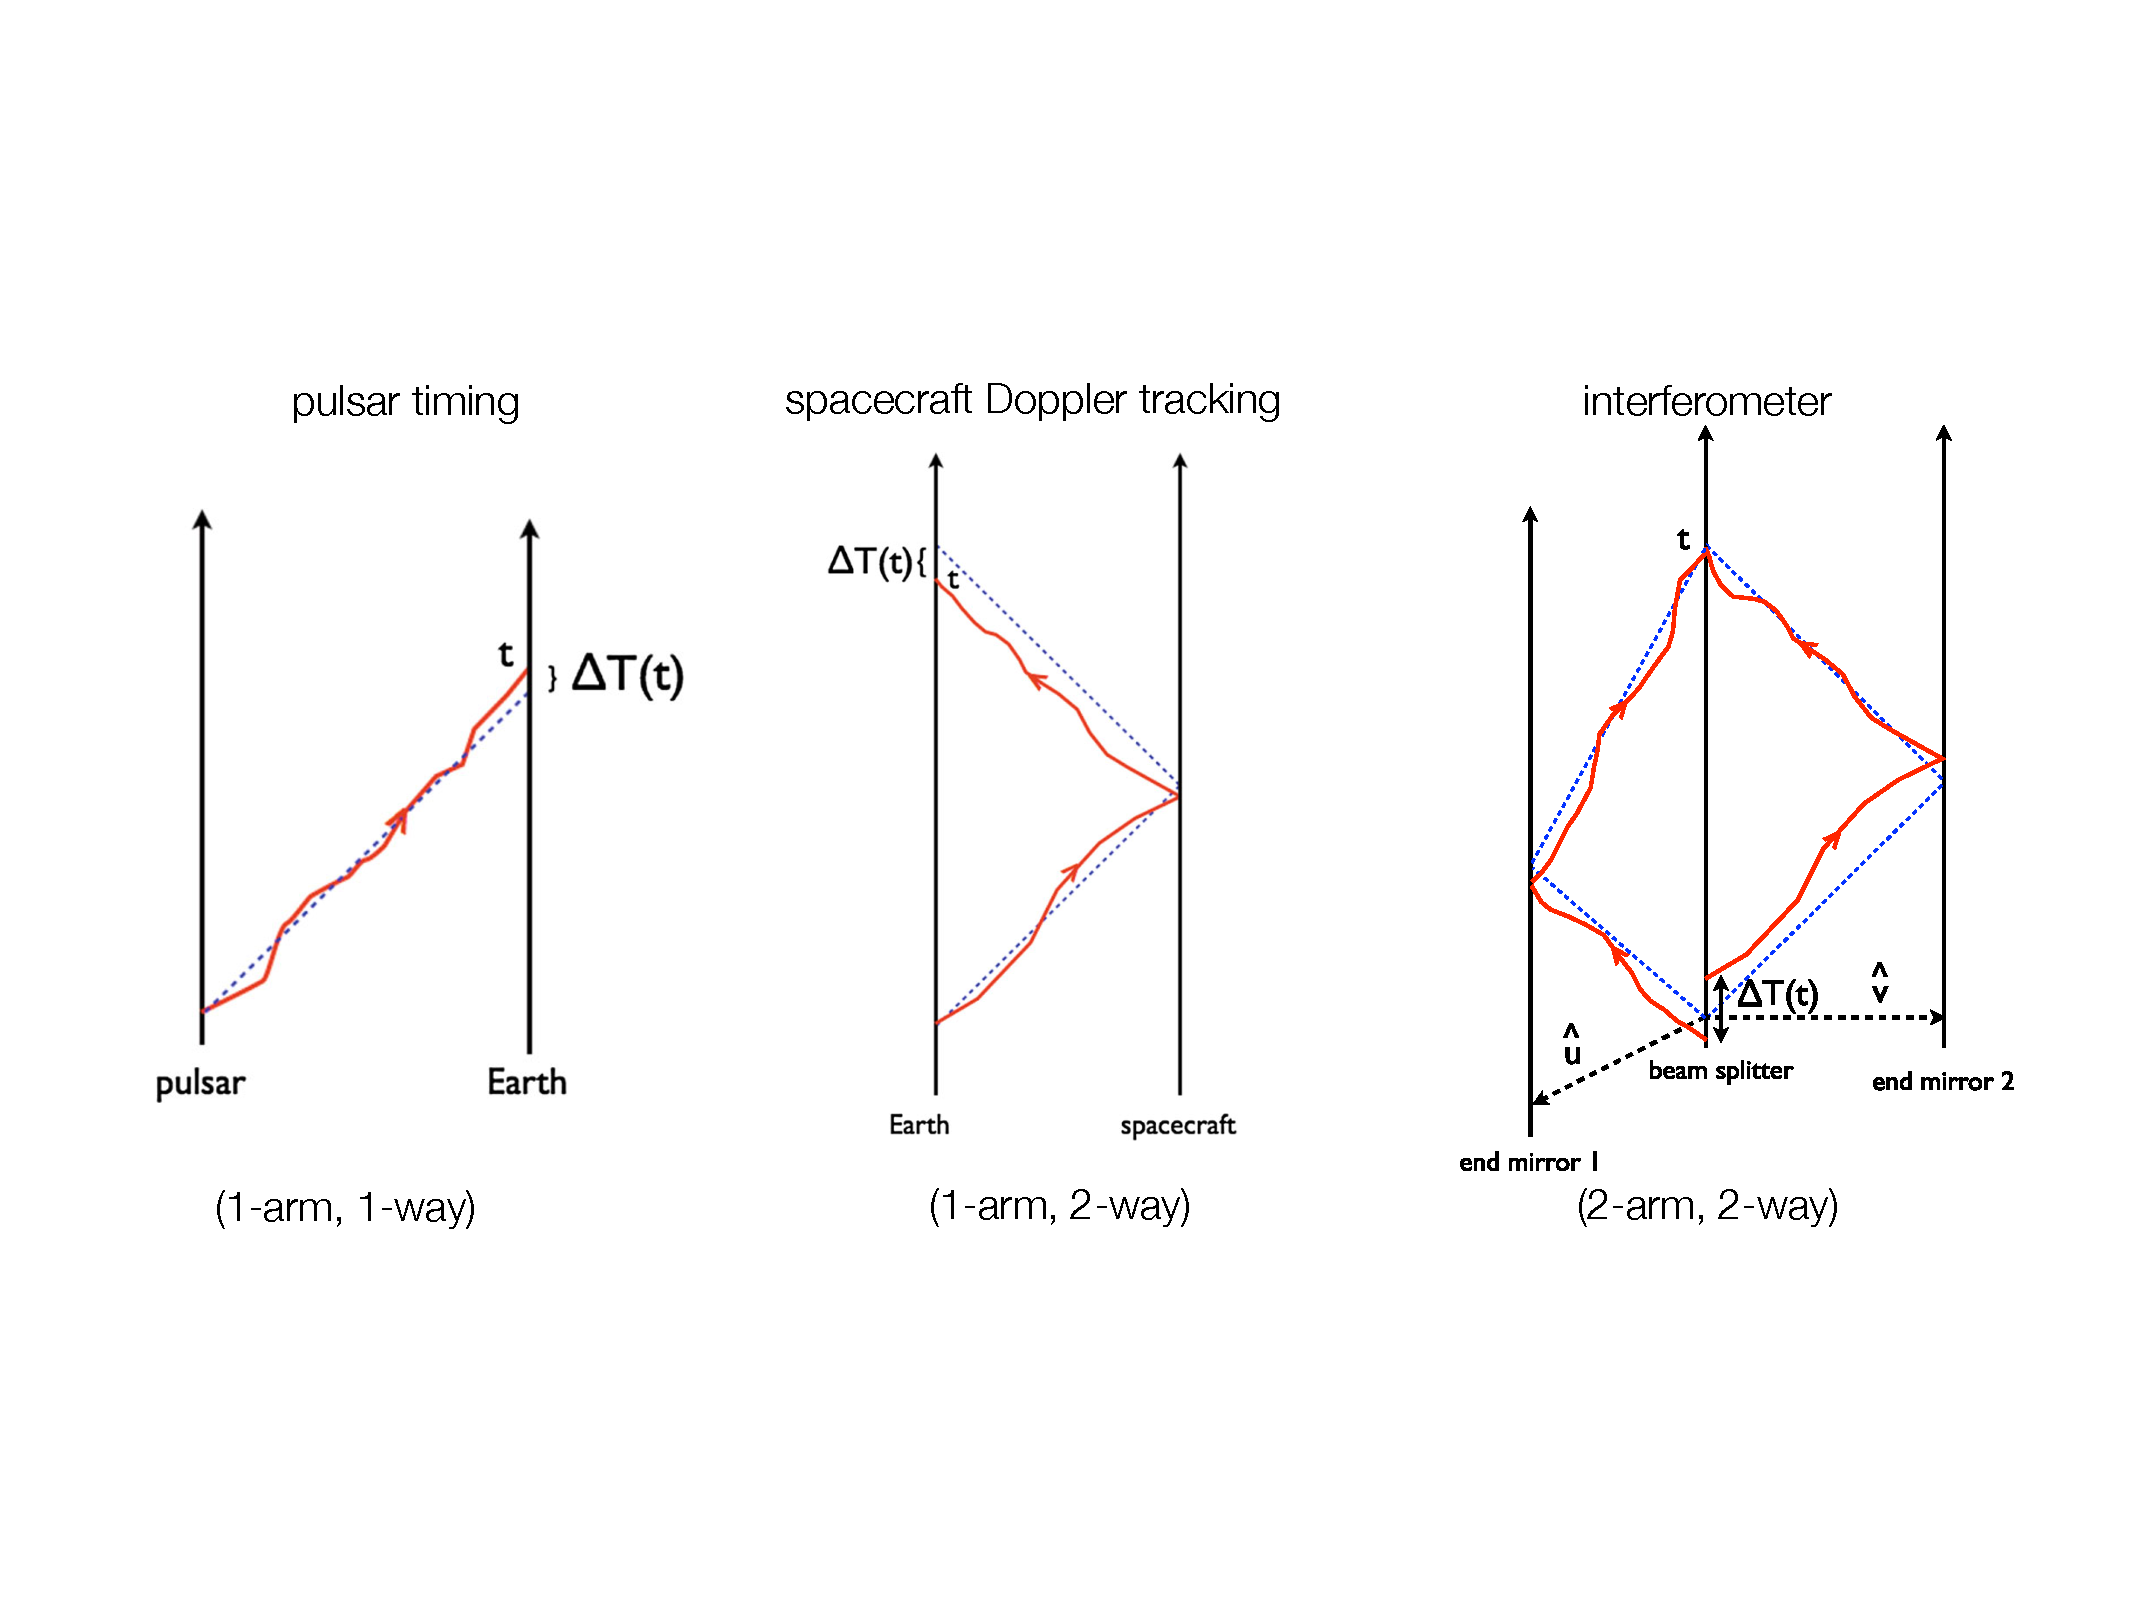
\includegraphics[width=\textwidth]{Figures/beam_detectors}
\caption{Spacetime diagram showing the response of beam
detectors to a passing GW.  
Left column: pulsar timing; middle column: spacecraft Doppler
tracking; right column: interferometer (ground or space-based).
A passing GW perturbs the path of the photon (red trajectory) 
relative to its nominal path in the absence of the wave 
(blue dotted line), leading to a 
difference in the expected arrival time of the photon.
(Figure adapted from \cite{Romano-Cornish:2017}.)}
\label{f:beam_detectors}
\end{center}
\end{figure}
%

In the literature, one might see the detector response
written in terms of strain $\Delta L(t)/L$, 
fractional Doppler frequency $\Delta v(t)/\nu_0$, or 
phase $\Delta\Phi(t)$, instead of the timing residual
$\Delta T(t)$.
Despite the apparent differences in the responses, 
they are all simply related to the timing residual 
response via the relations:
%
\be
\begin{aligned}
&h(t)\equiv \Delta T(t)\quad &({\rm pulsar\ timing})\\
&h(t)\equiv \frac{\Delta L(t)}{L} = \frac{\Delta T(t)}{T}
\quad&({\rm LIGO,\ Virgo,\ }\cdots) \\
&h(t)\equiv \frac{\Delta\nu(t)}{\nu_0}=\frac{\D \Delta T(t)}{\D t}
\quad &({\rm spacecraft Doppler\ tracking})\\
&h(t)\equiv \Delta\Phi(t) = 2\pi \nu_0\,\Delta T(t)
\quad &({\rm LISA})\,.
\end{aligned}
\ee
%
Hence, once we know how to calculate the timing residual
response $\Delta T(t)$, we can easily calculate all the
other quantities listed above.

\begin{figure}[htbp!]
\begin{center}
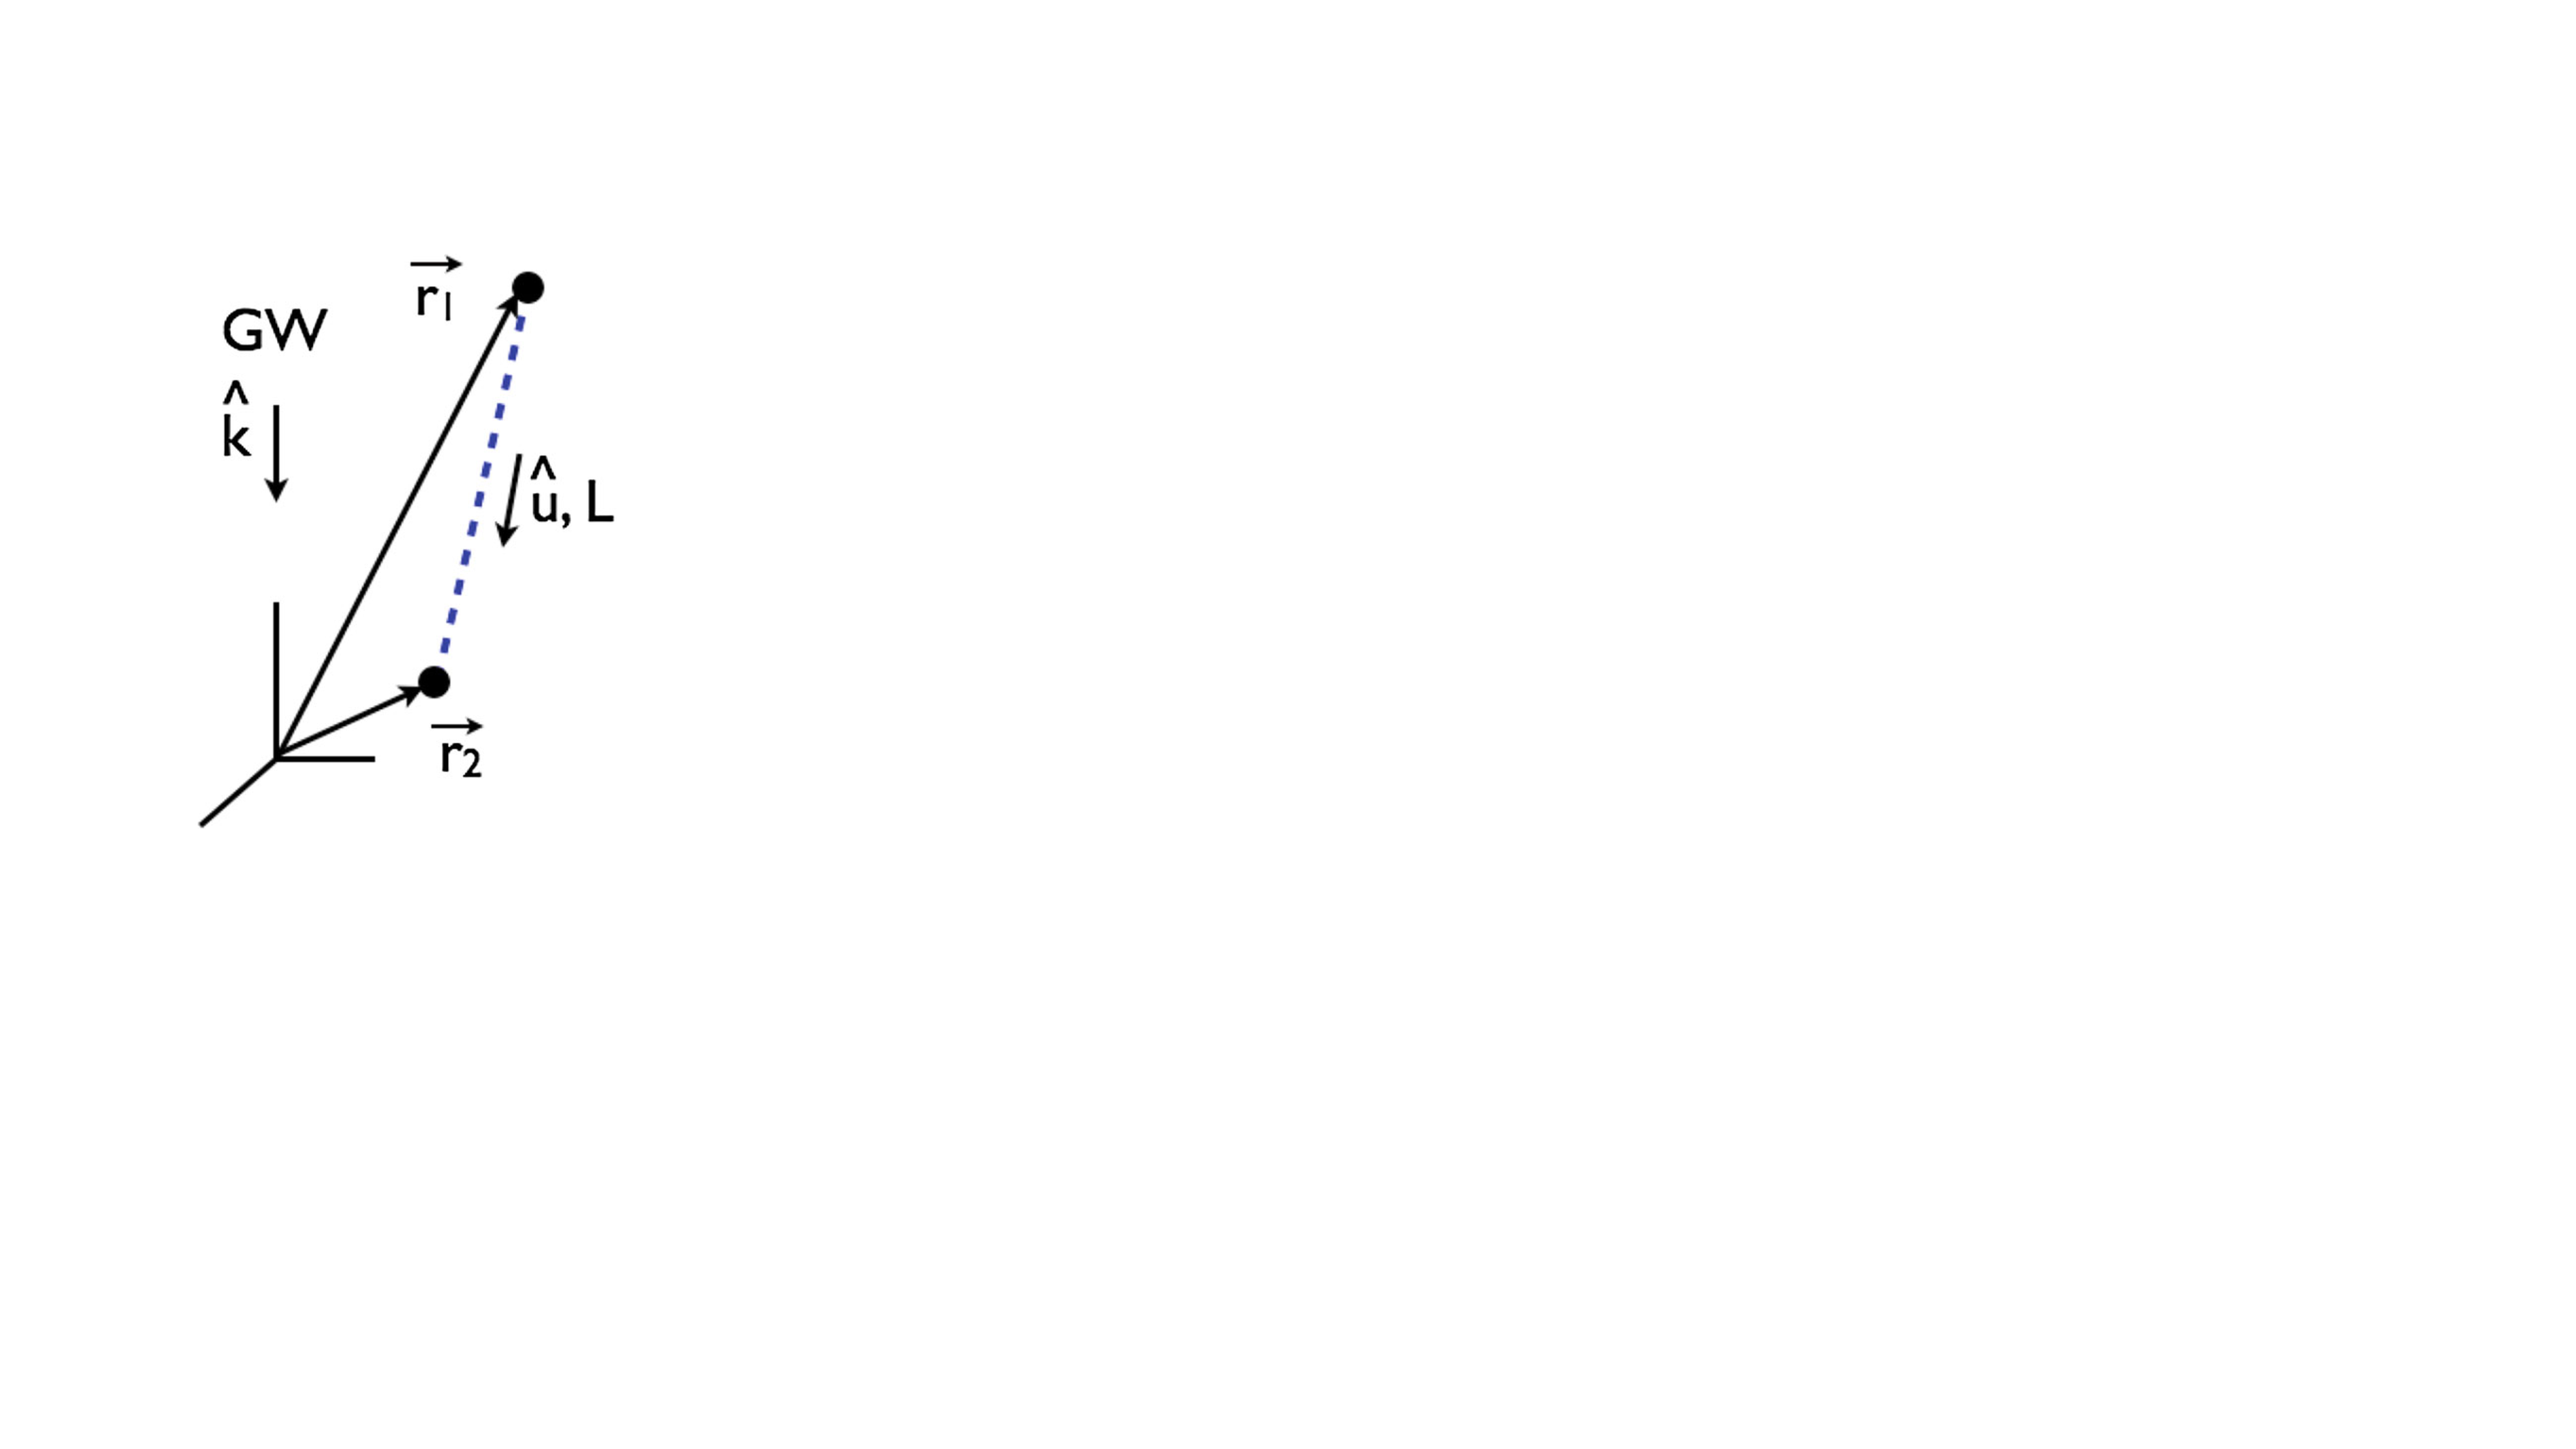
\includegraphics[width=0.2\textwidth]{Figures/one_arm_one_way}
\caption{Geometry for a one-arm, one-way beam detector, relevant for 
a pulsar timing residual measurement.
The GW propagates in the $\hat k$ direction; the electromagnetic wave
(e.g., a radio pulse from a pulsar) propagates in the $\hat u$ direction
(opposite of the direction to the pulsar, $\hat p=-\hat u$.} 
\label{f:one_arm_one_way}
\end{center}
\end{figure}

\begin{figure}[htbp!]
\begin{center}
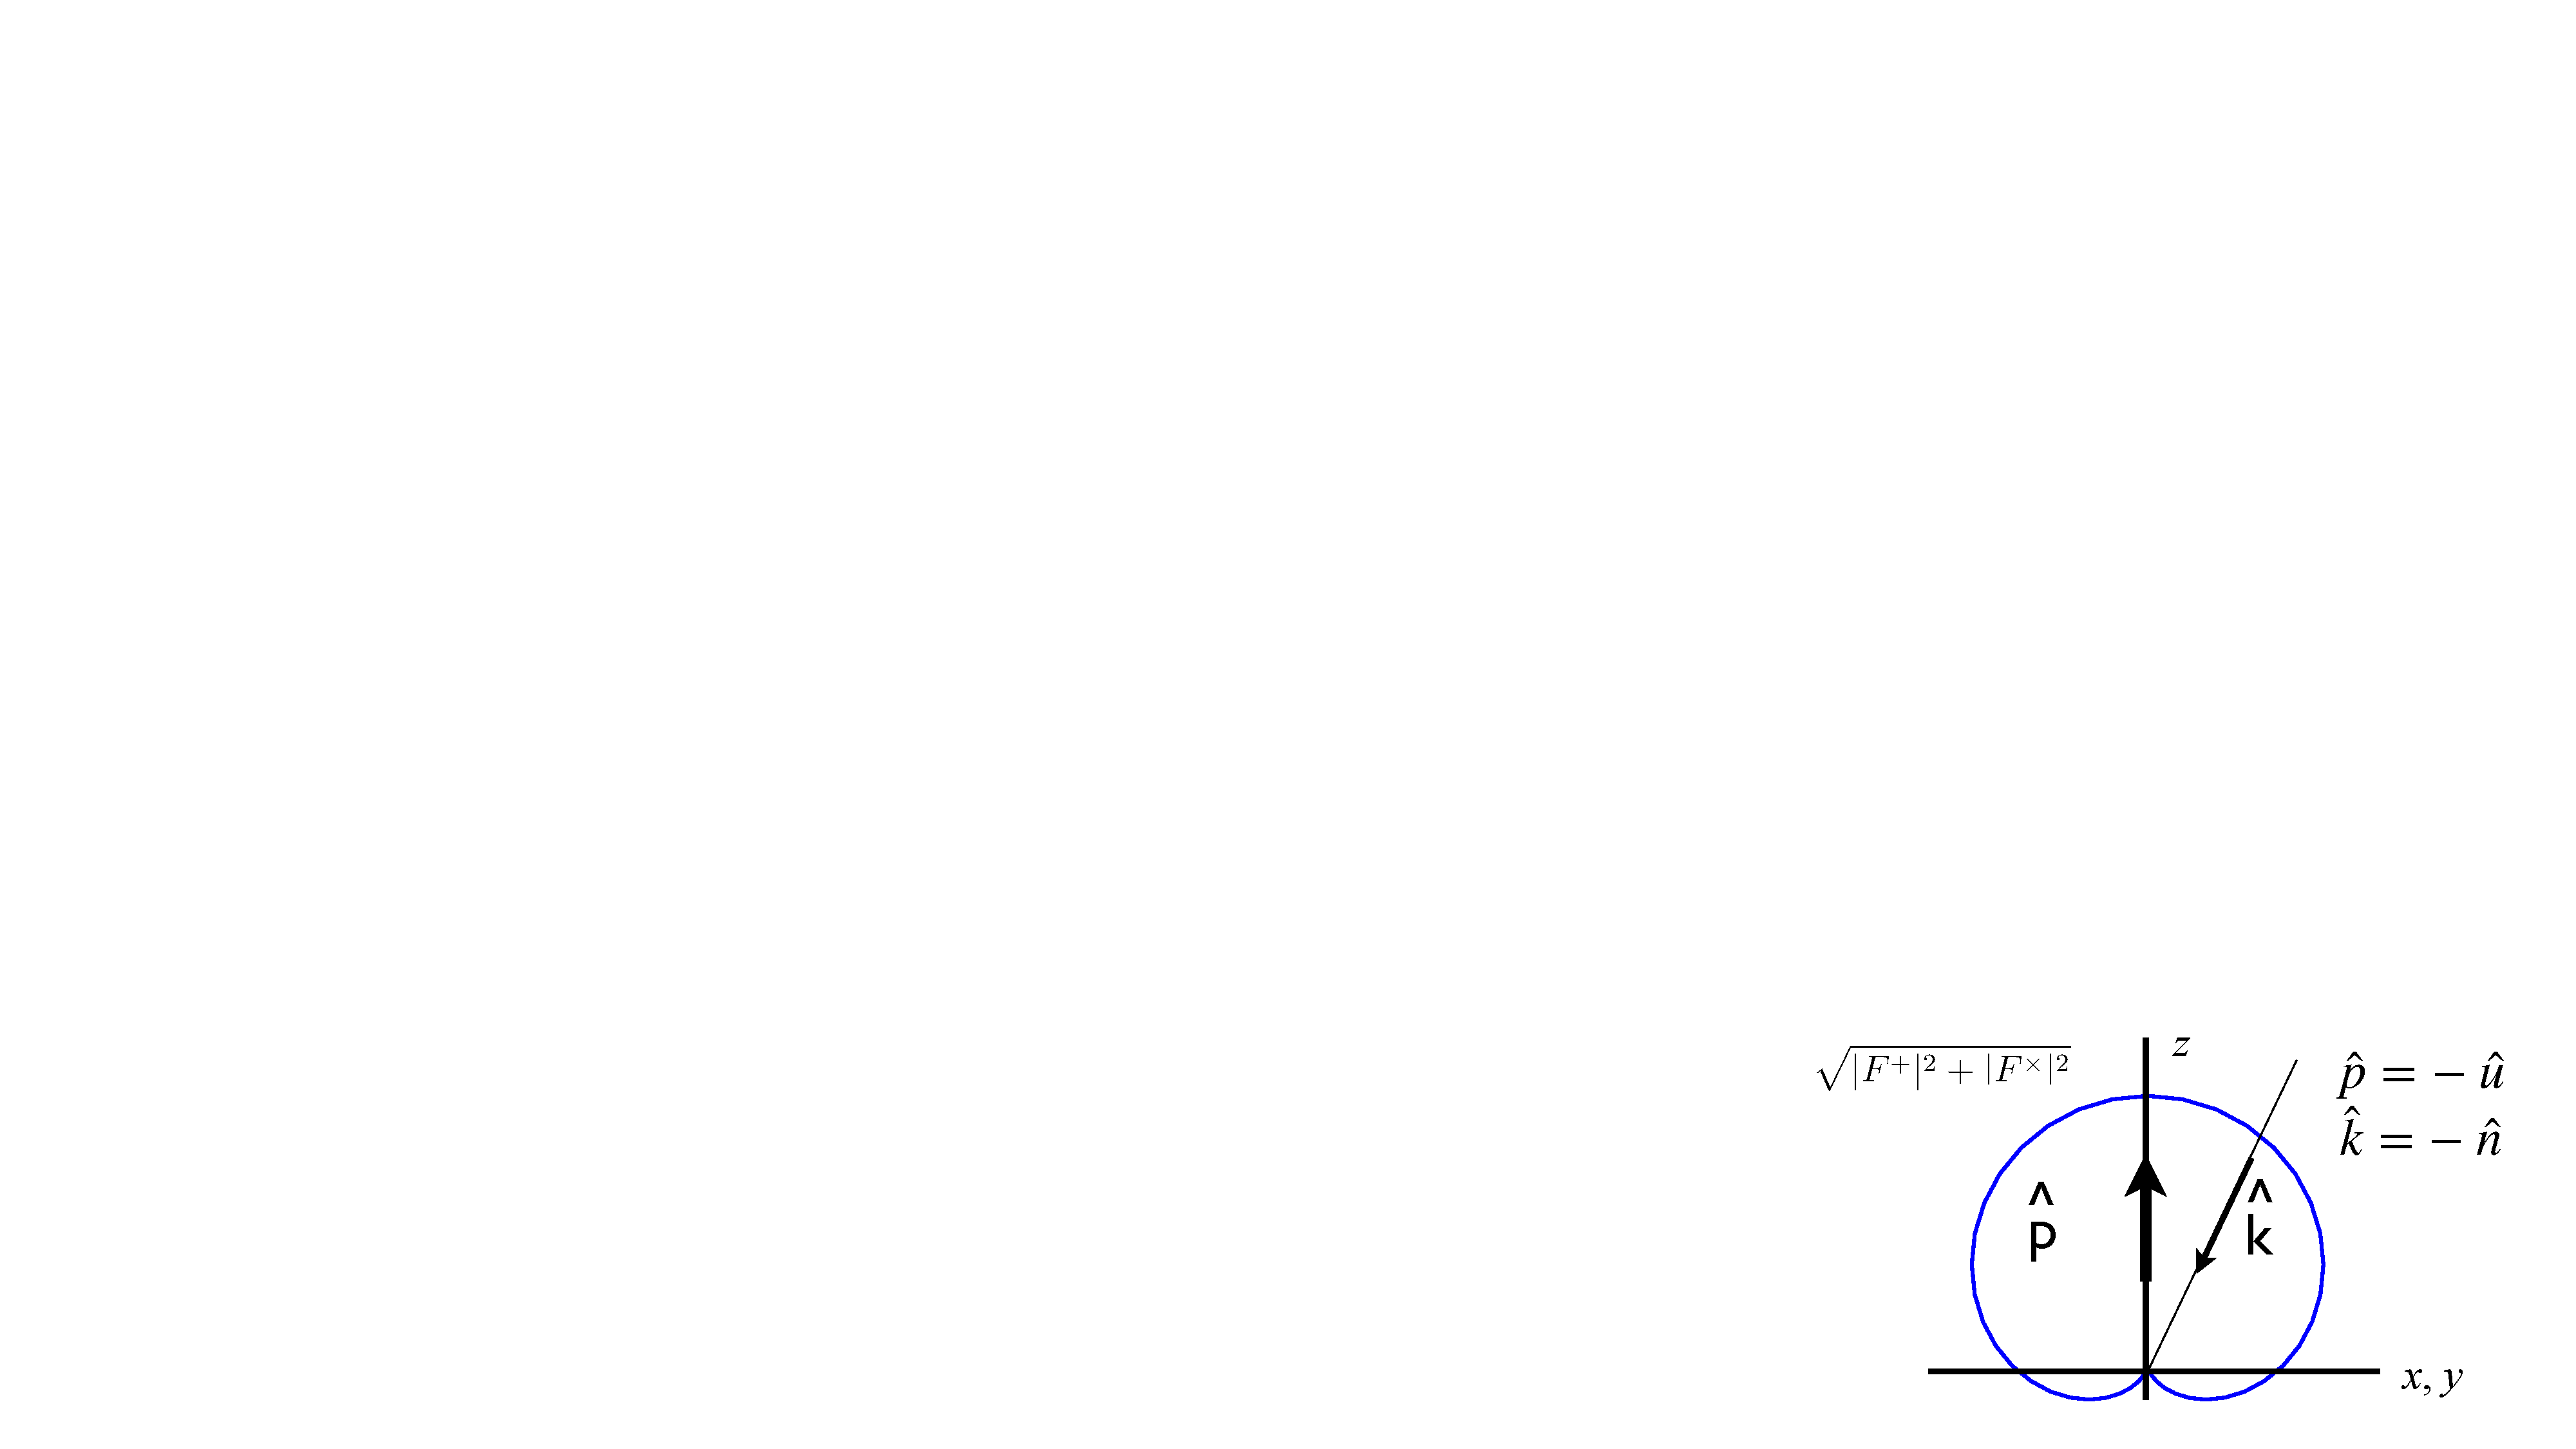
\includegraphics[width=0.4\textwidth]{Figures/one_arm_one_way_peanut}
\caption{Polarization averaged response 
$\sqrt{|F^+(\hat k)|^2+|F_\times(\hat k)|^2}$
for pulsar timing residuals ignoring the pulsar term and the 
frequency-dependent factor $1/(2\pi f)$ out front.
The response is axially symmetric around the $z$-axis, which
we've chose to be the direction to the pulsar.}
\label{f:one_arm_one_way_peanut}
\end{center}
\end{figure}

\begin{figure}[htbp!]
\begin{center}
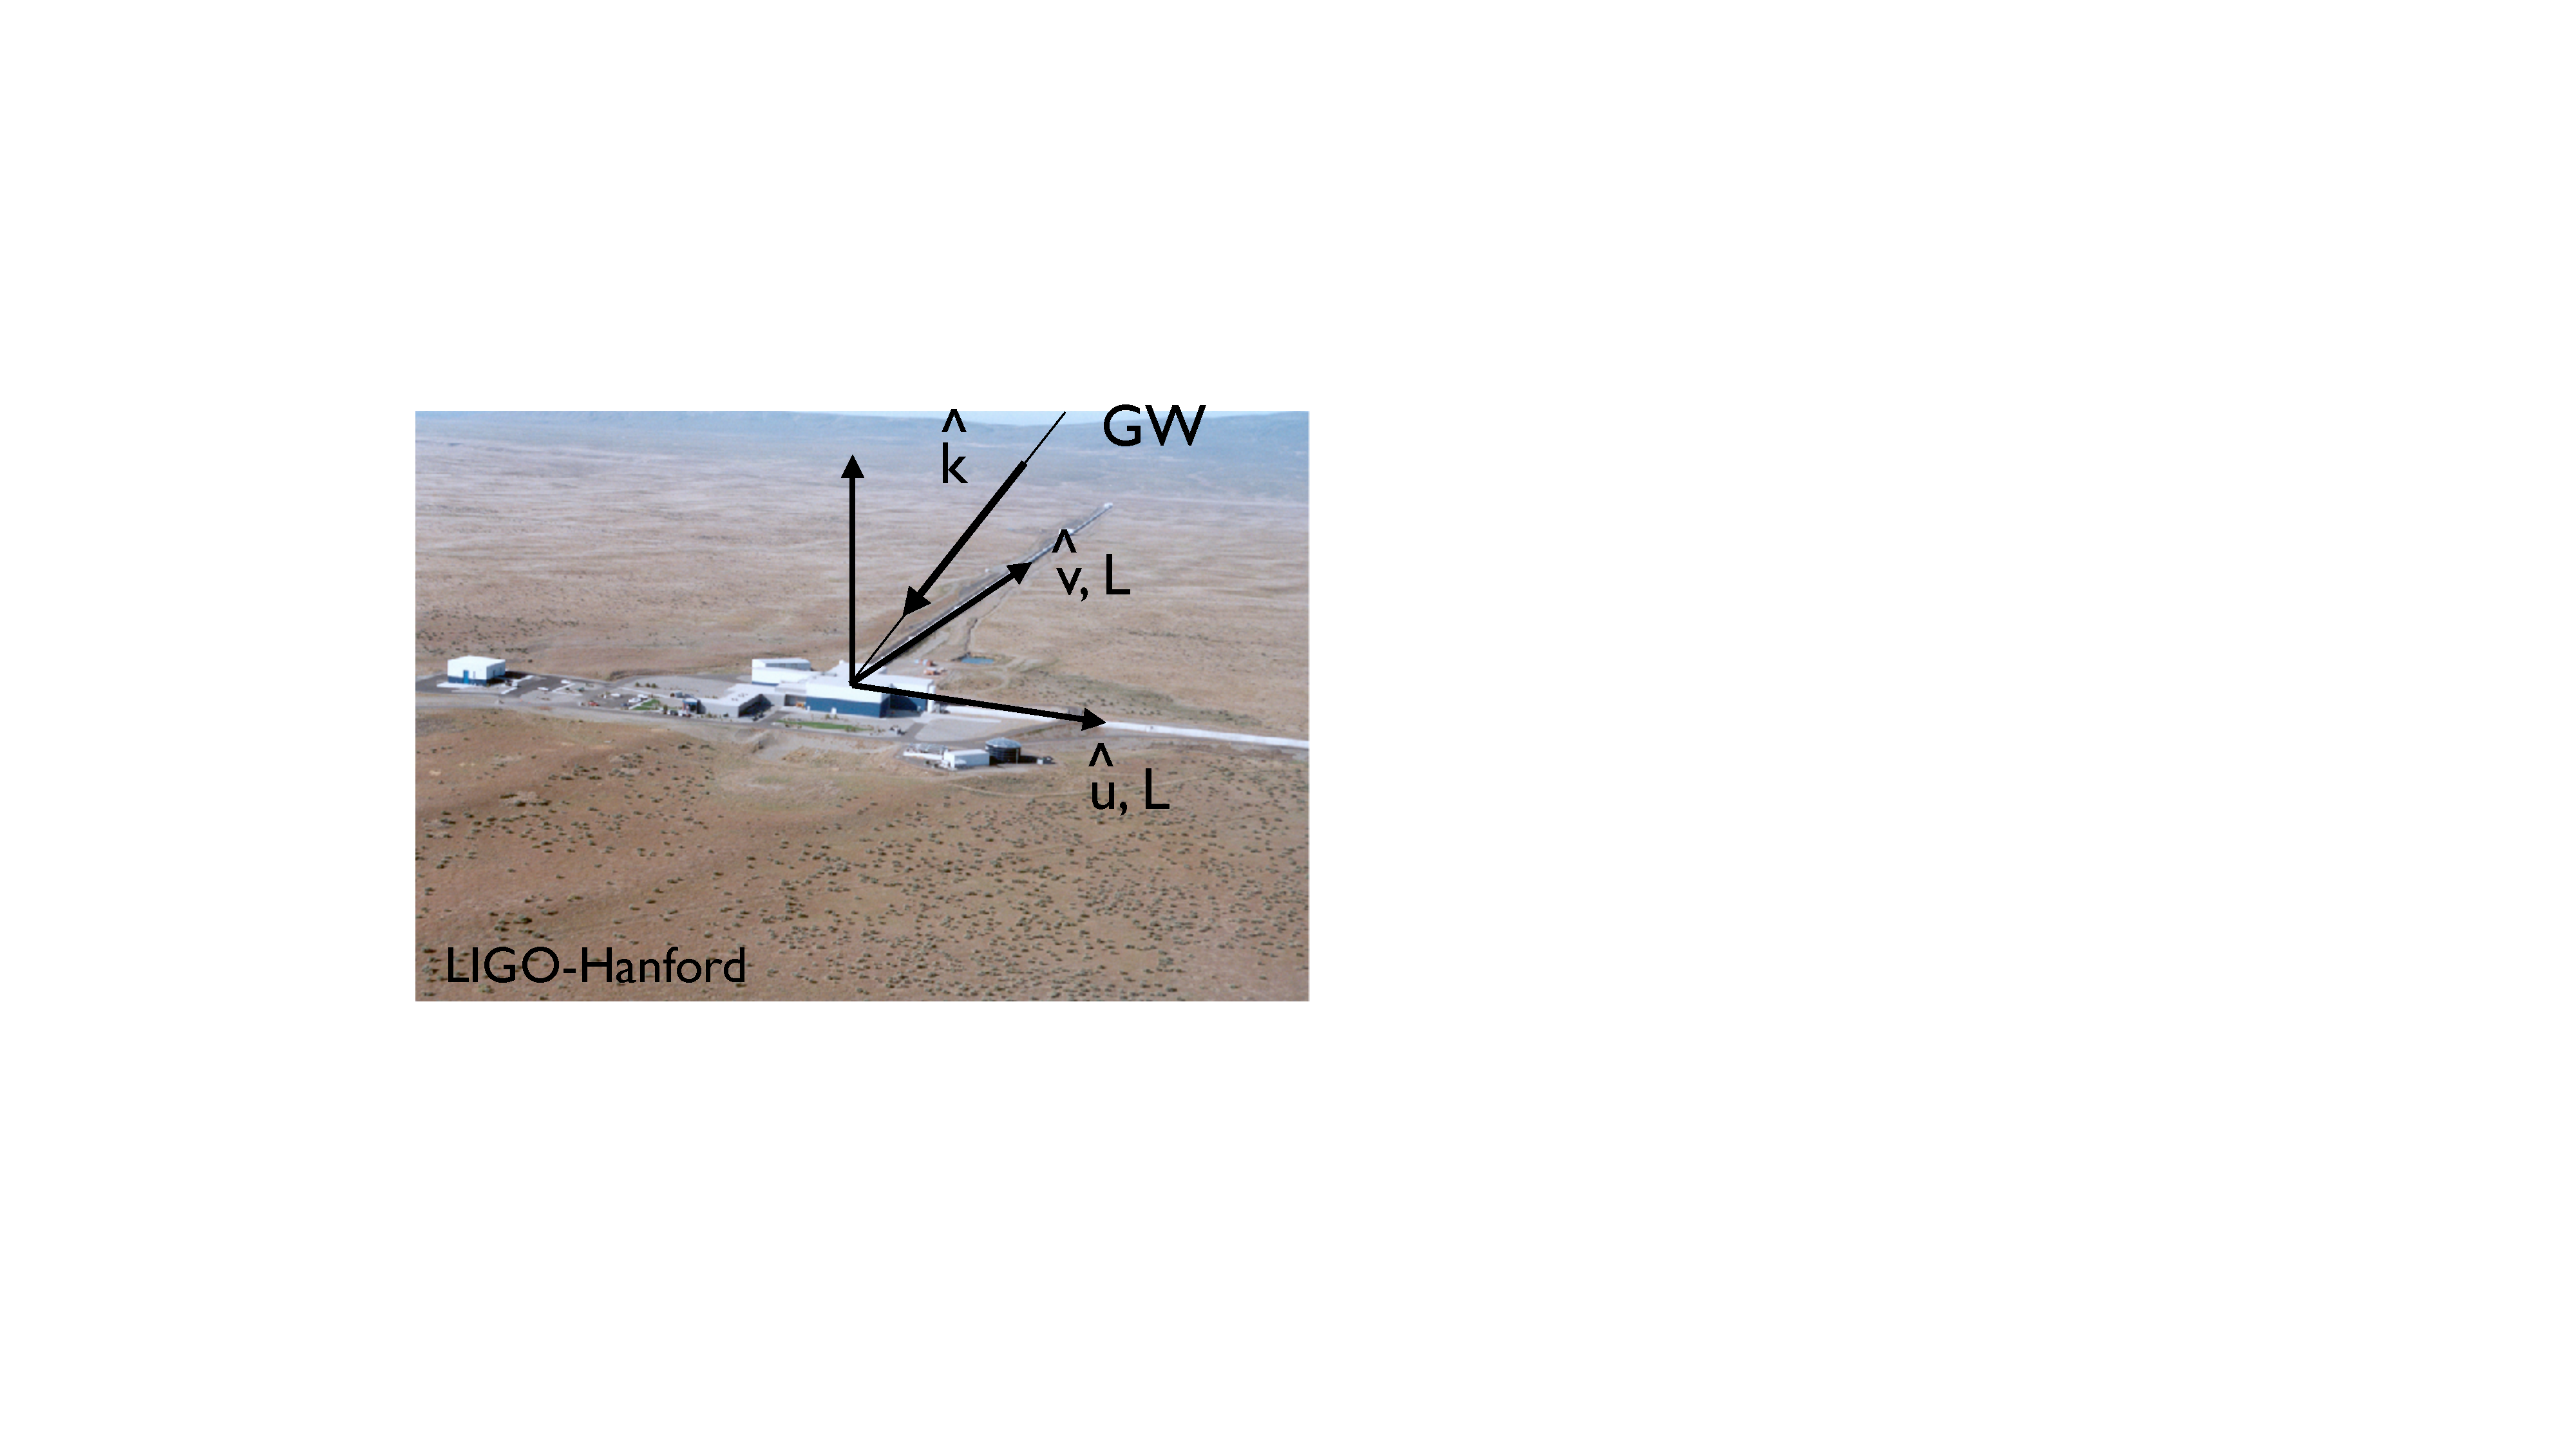
\includegraphics[width=0.6\textwidth]{Figures/LHO_geometry}
\caption{Geometry for a ground-based interferometer GW response
calculation.
(Shown here the LIGO Hanford Observatory, in Hanford, WA.)
The GW propagates in the $\hat k$ direction;
$\hat u$, $\hat v$ are unit vectors that point along the 
two arms of the interferometer.
In the short-antenna approximation, the length $L$ of the 
arms does not enter the expression for the response function.}
\label{f:LHO_geometry}
\end{center}
\end{figure}

\begin{figure}[htbp!]
\begin{center}
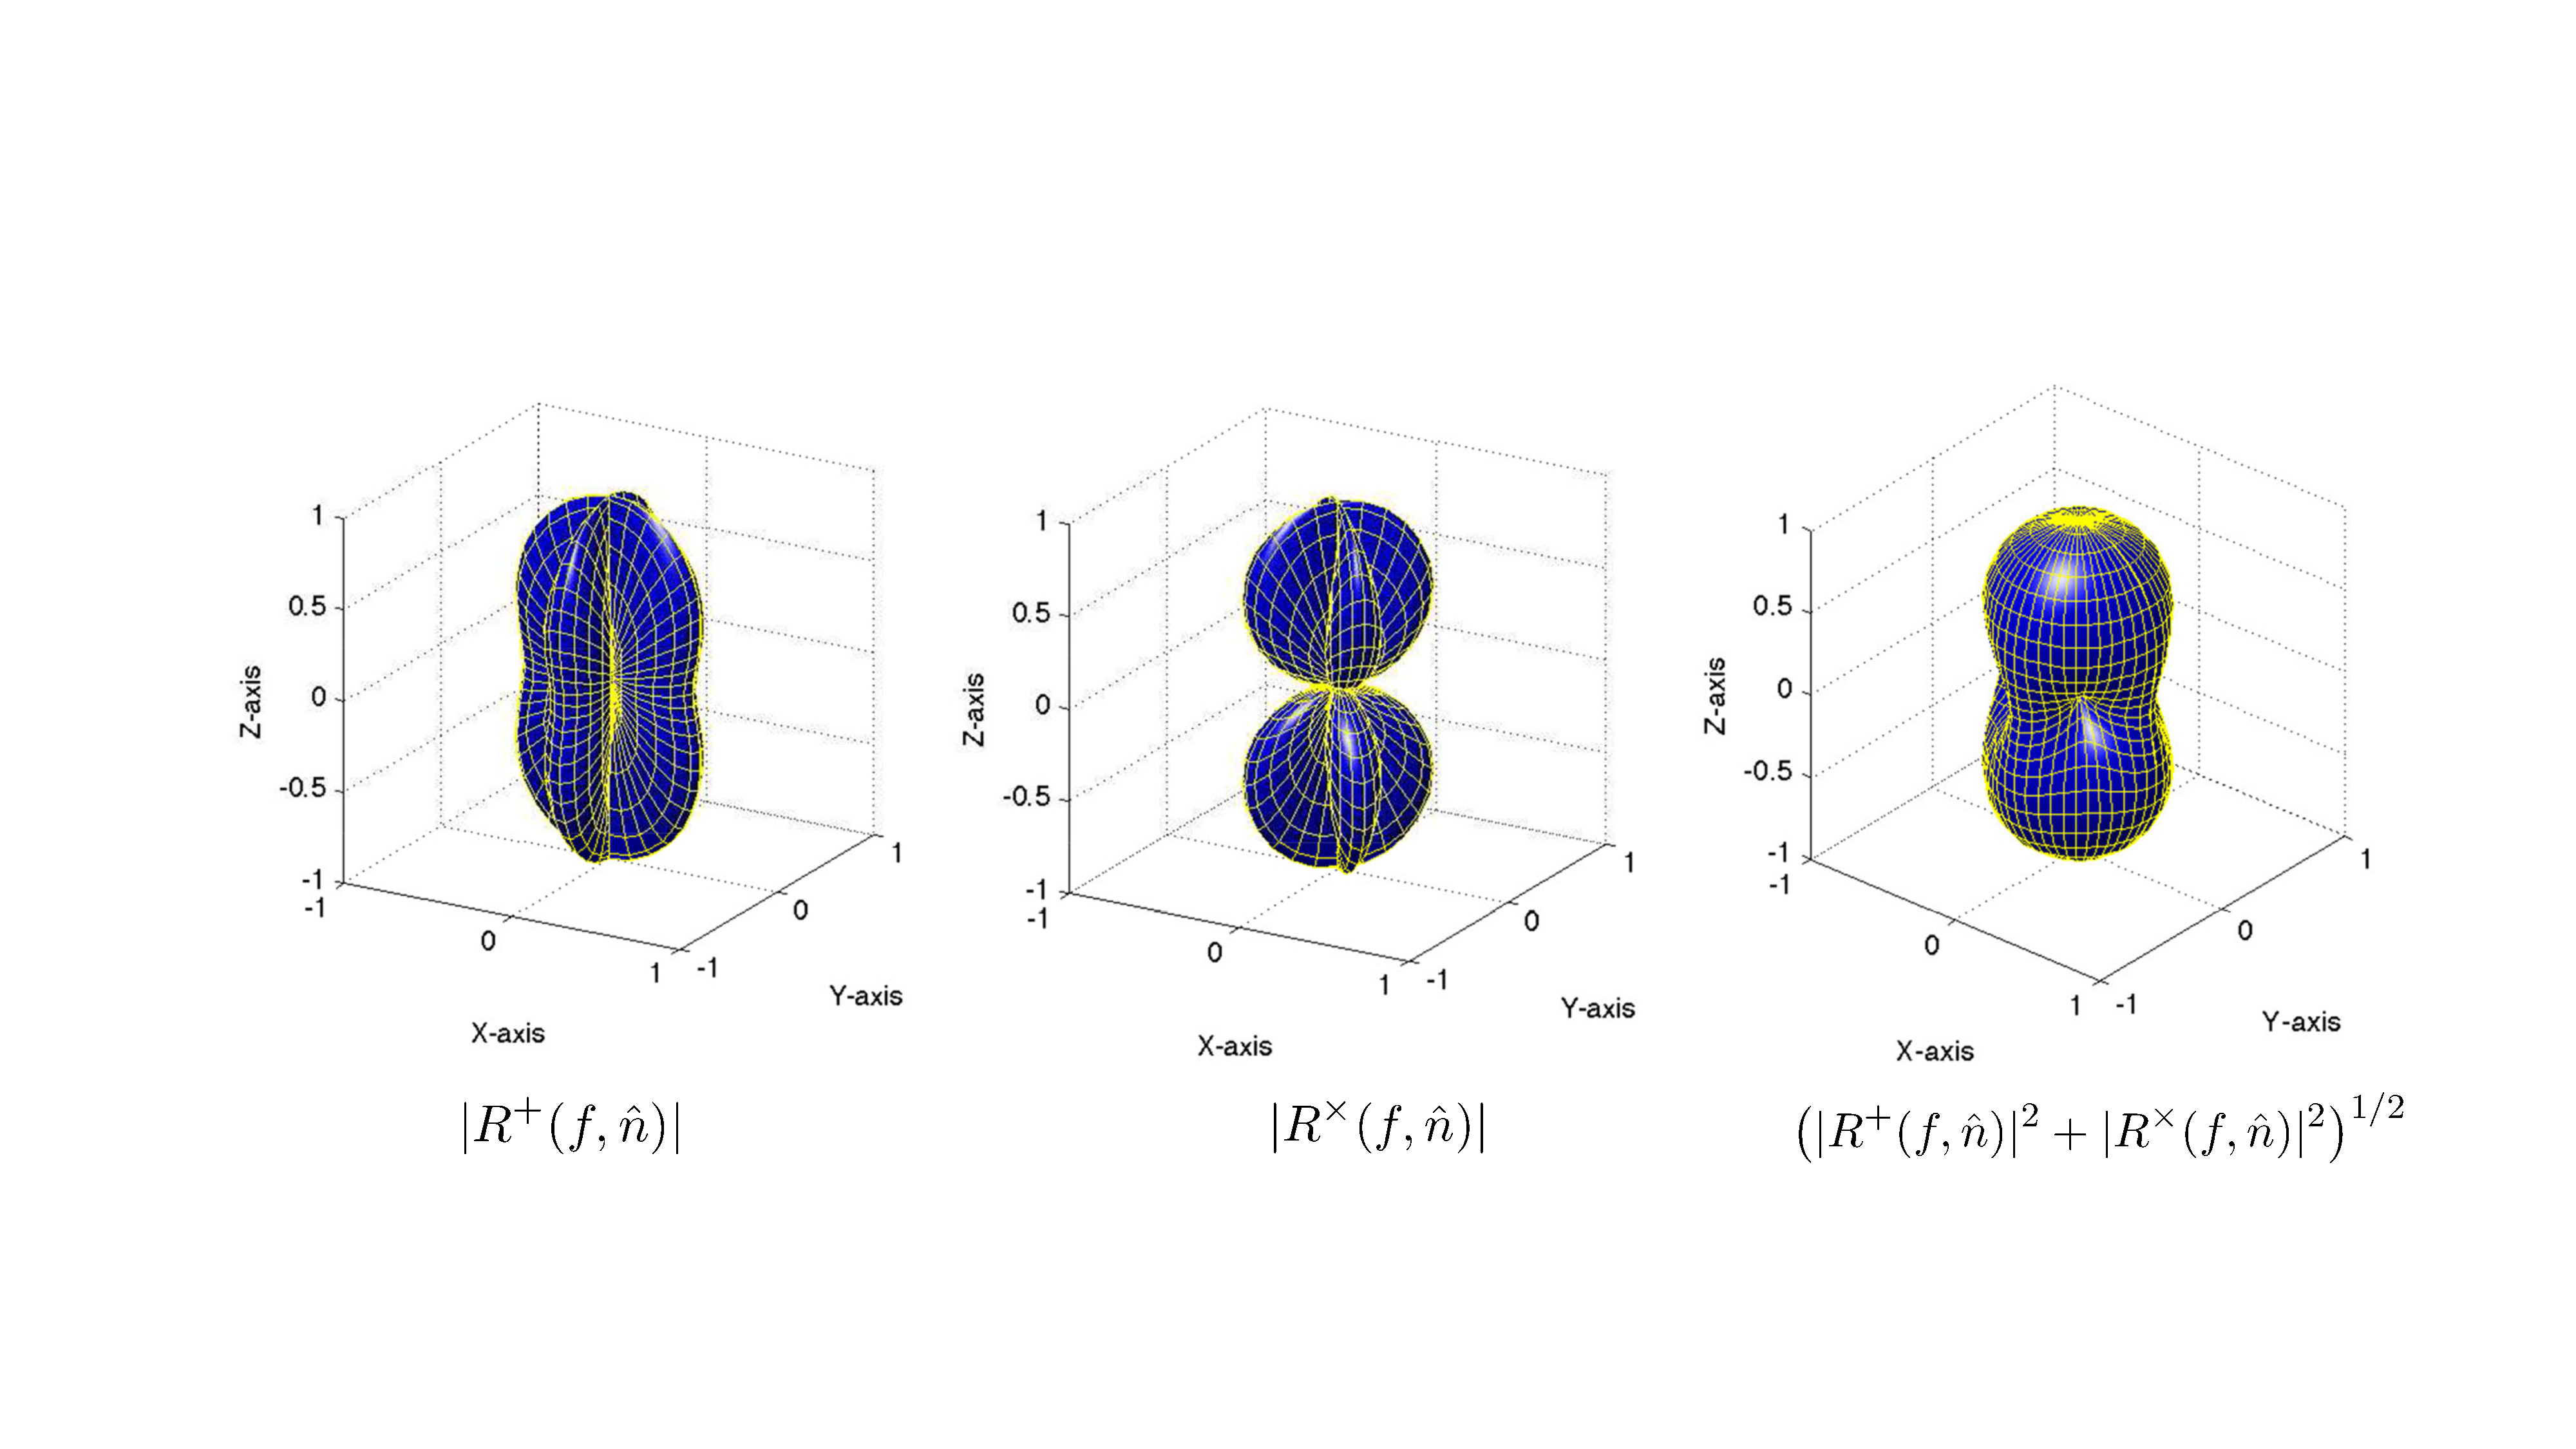
\includegraphics[width=\textwidth]{Figures/LIGO_beam_patterns}
\caption{Beam pattern functions for a ground-based interferometer
like LIGO in the short-antenna approximation---i.e., $f\lesssim {\rm few\ kHz}$.
The vertex of the interferometer is at the origin of coordinates,
and interferometer arms are assumed to be orthogonal pointing along
the $x$ and $y$ directions.}
\label{f:LIGO_beam_patterns}
\end{center}
\end{figure}

%%%%%%%%%%%%%%%%%%%%%%%%%%%%%%%%%%%%%%%%%%%%%%%%%%%%%%%
\section{Non-trivial correlations}
\label{s:nontrivial_correlations}

Note that the first zero crossing occurs at roughly
60~Hz, corresponding to GW with wavelength equal to 
twice the separation between the two observatories.

\begin{figure}[htbp!]
\begin{center}
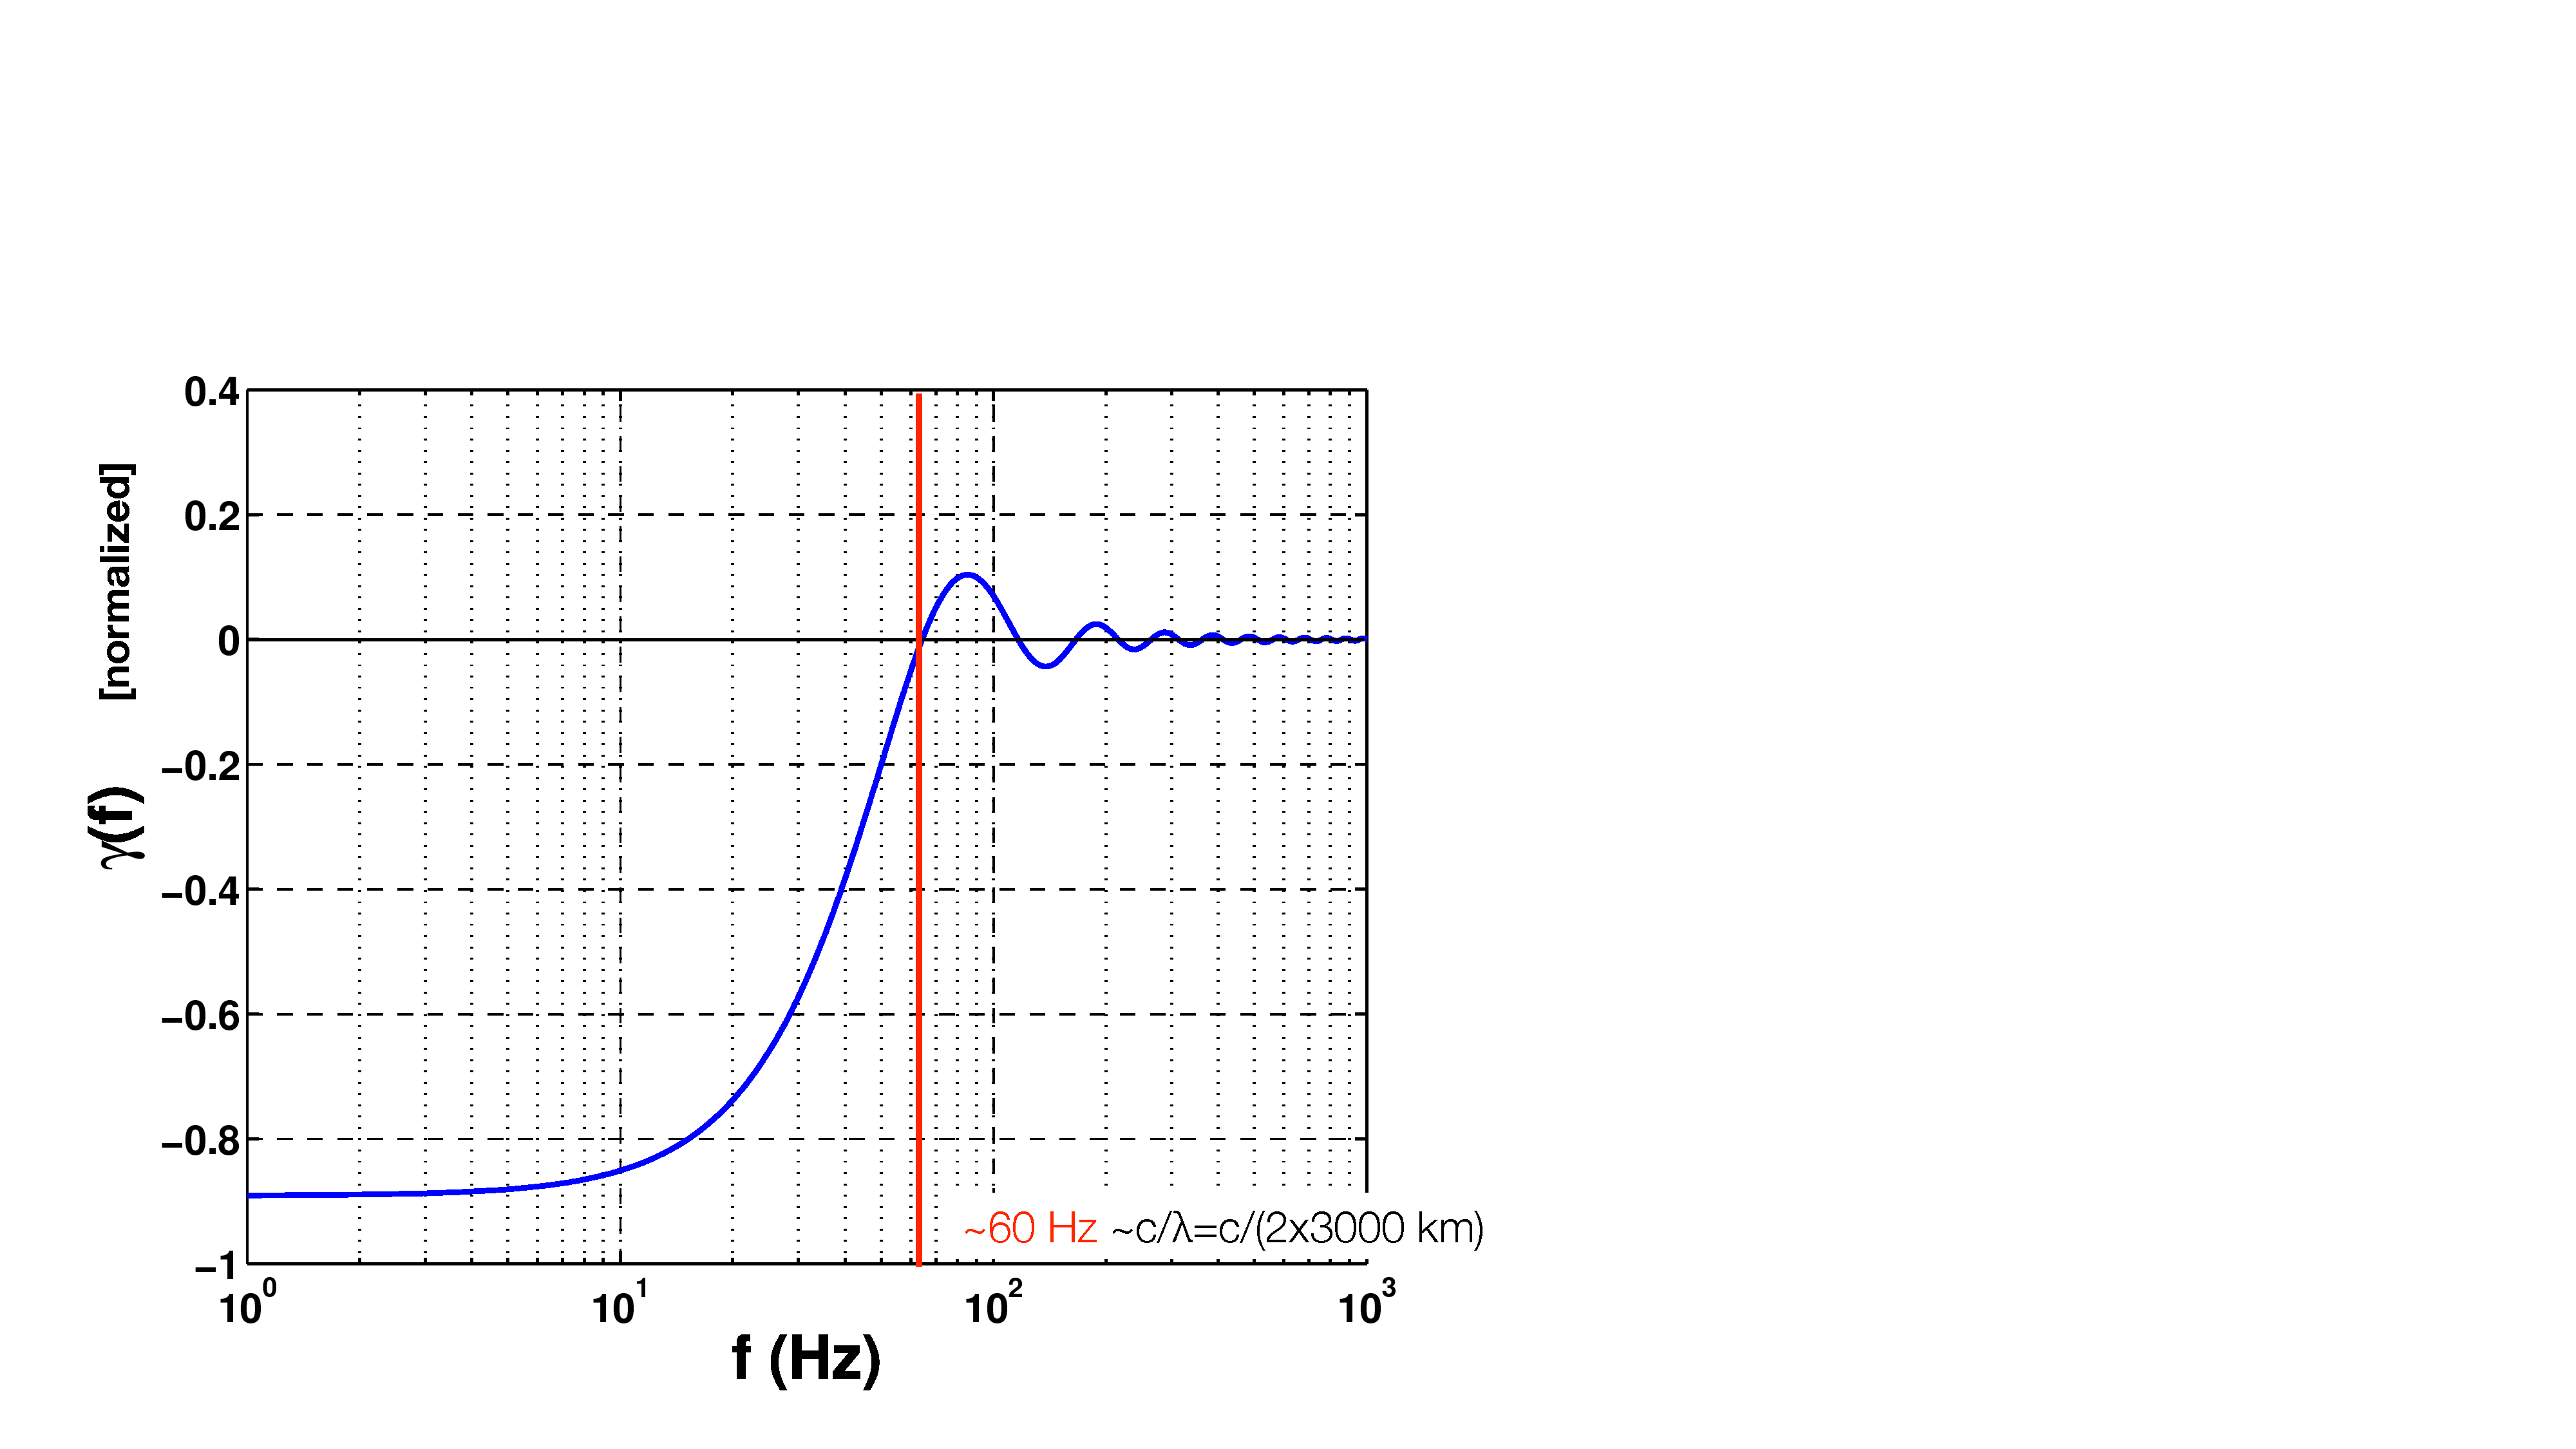
\includegraphics[width=0.49\textwidth]{Figures/LHO-LLO-orf}
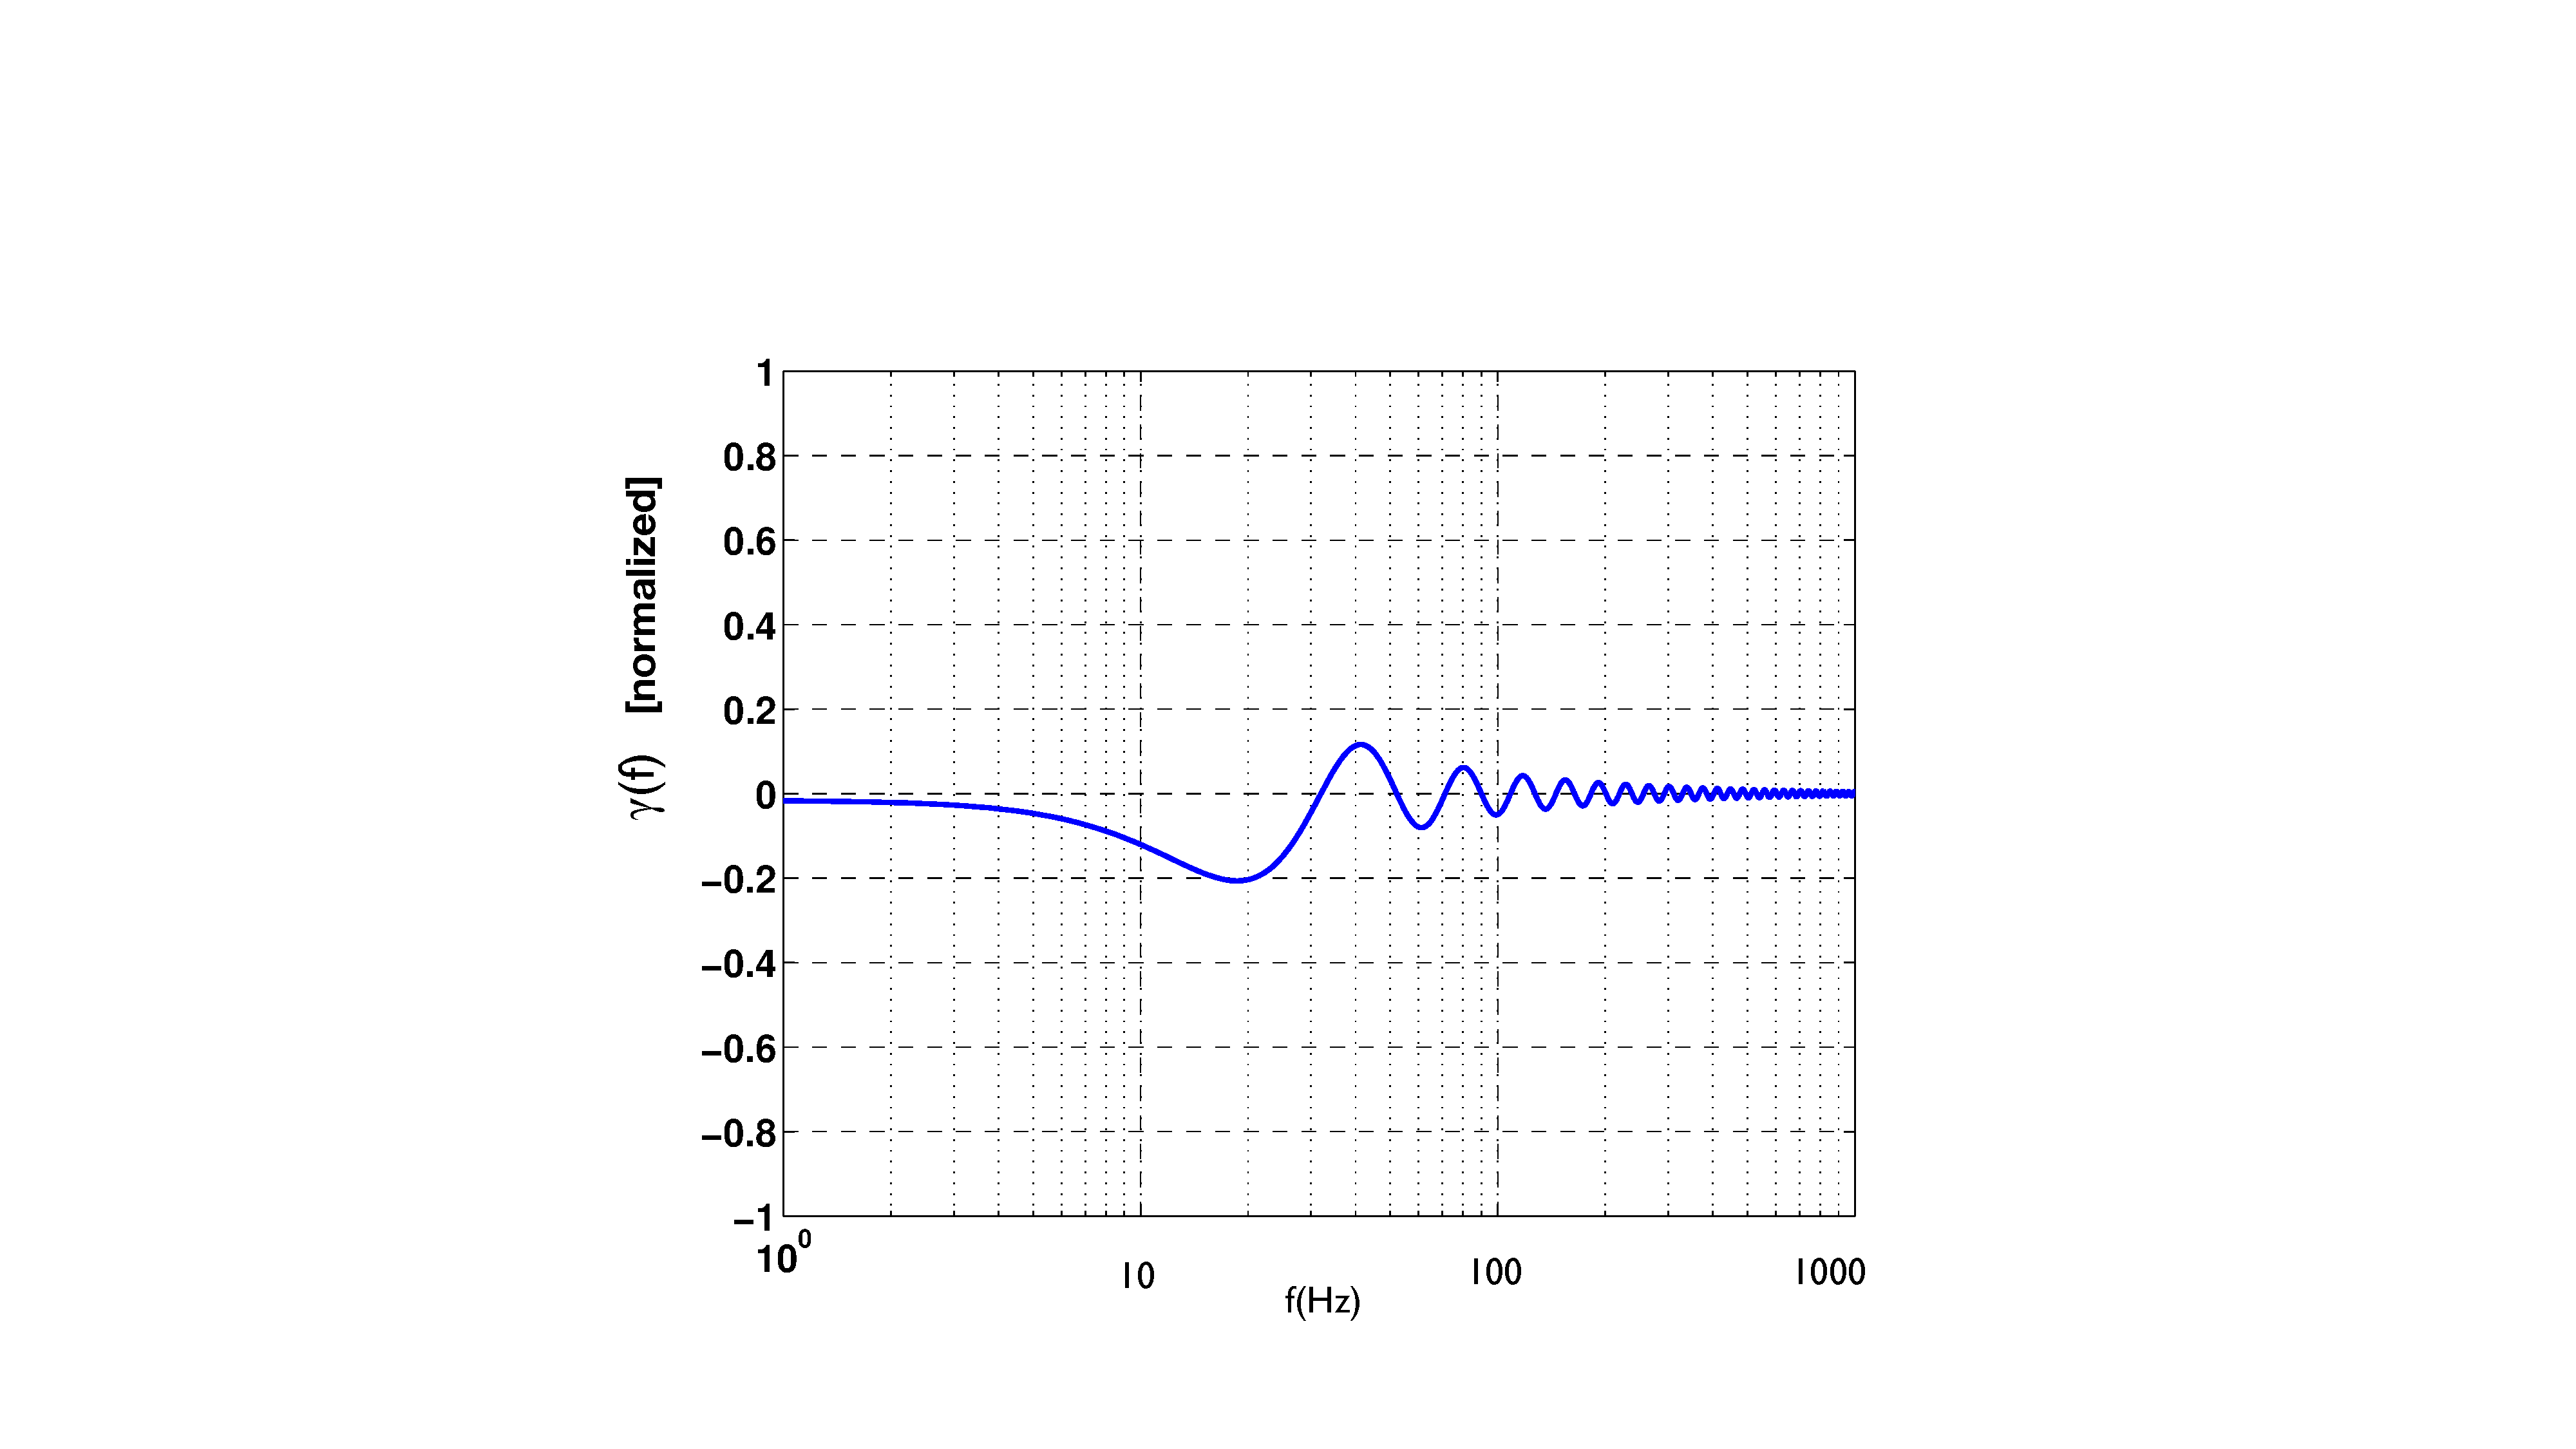
\includegraphics[width=0.49\textwidth]{Figures/LHO-Virgo-orf}
\caption{Normalized overlap function for ground-based
interferometers.
Left panel: LIGO Hanford-LIGO Livingston detector pair.
Rght panel: LIGO Hanford-Virgo detector pair.
These overlap functions were calculated in the small-antenna
approximation.
Note the reduced amplitude of the LHO-Virgo overlap function
relative to the LHO-LLO overlap function due to the much larger 
separation between Hanford, WA and Pisa, Italy.}
\label{f:orfs}
\end{center}
\end{figure}

\begin{figure}[htbp!]
\begin{center}
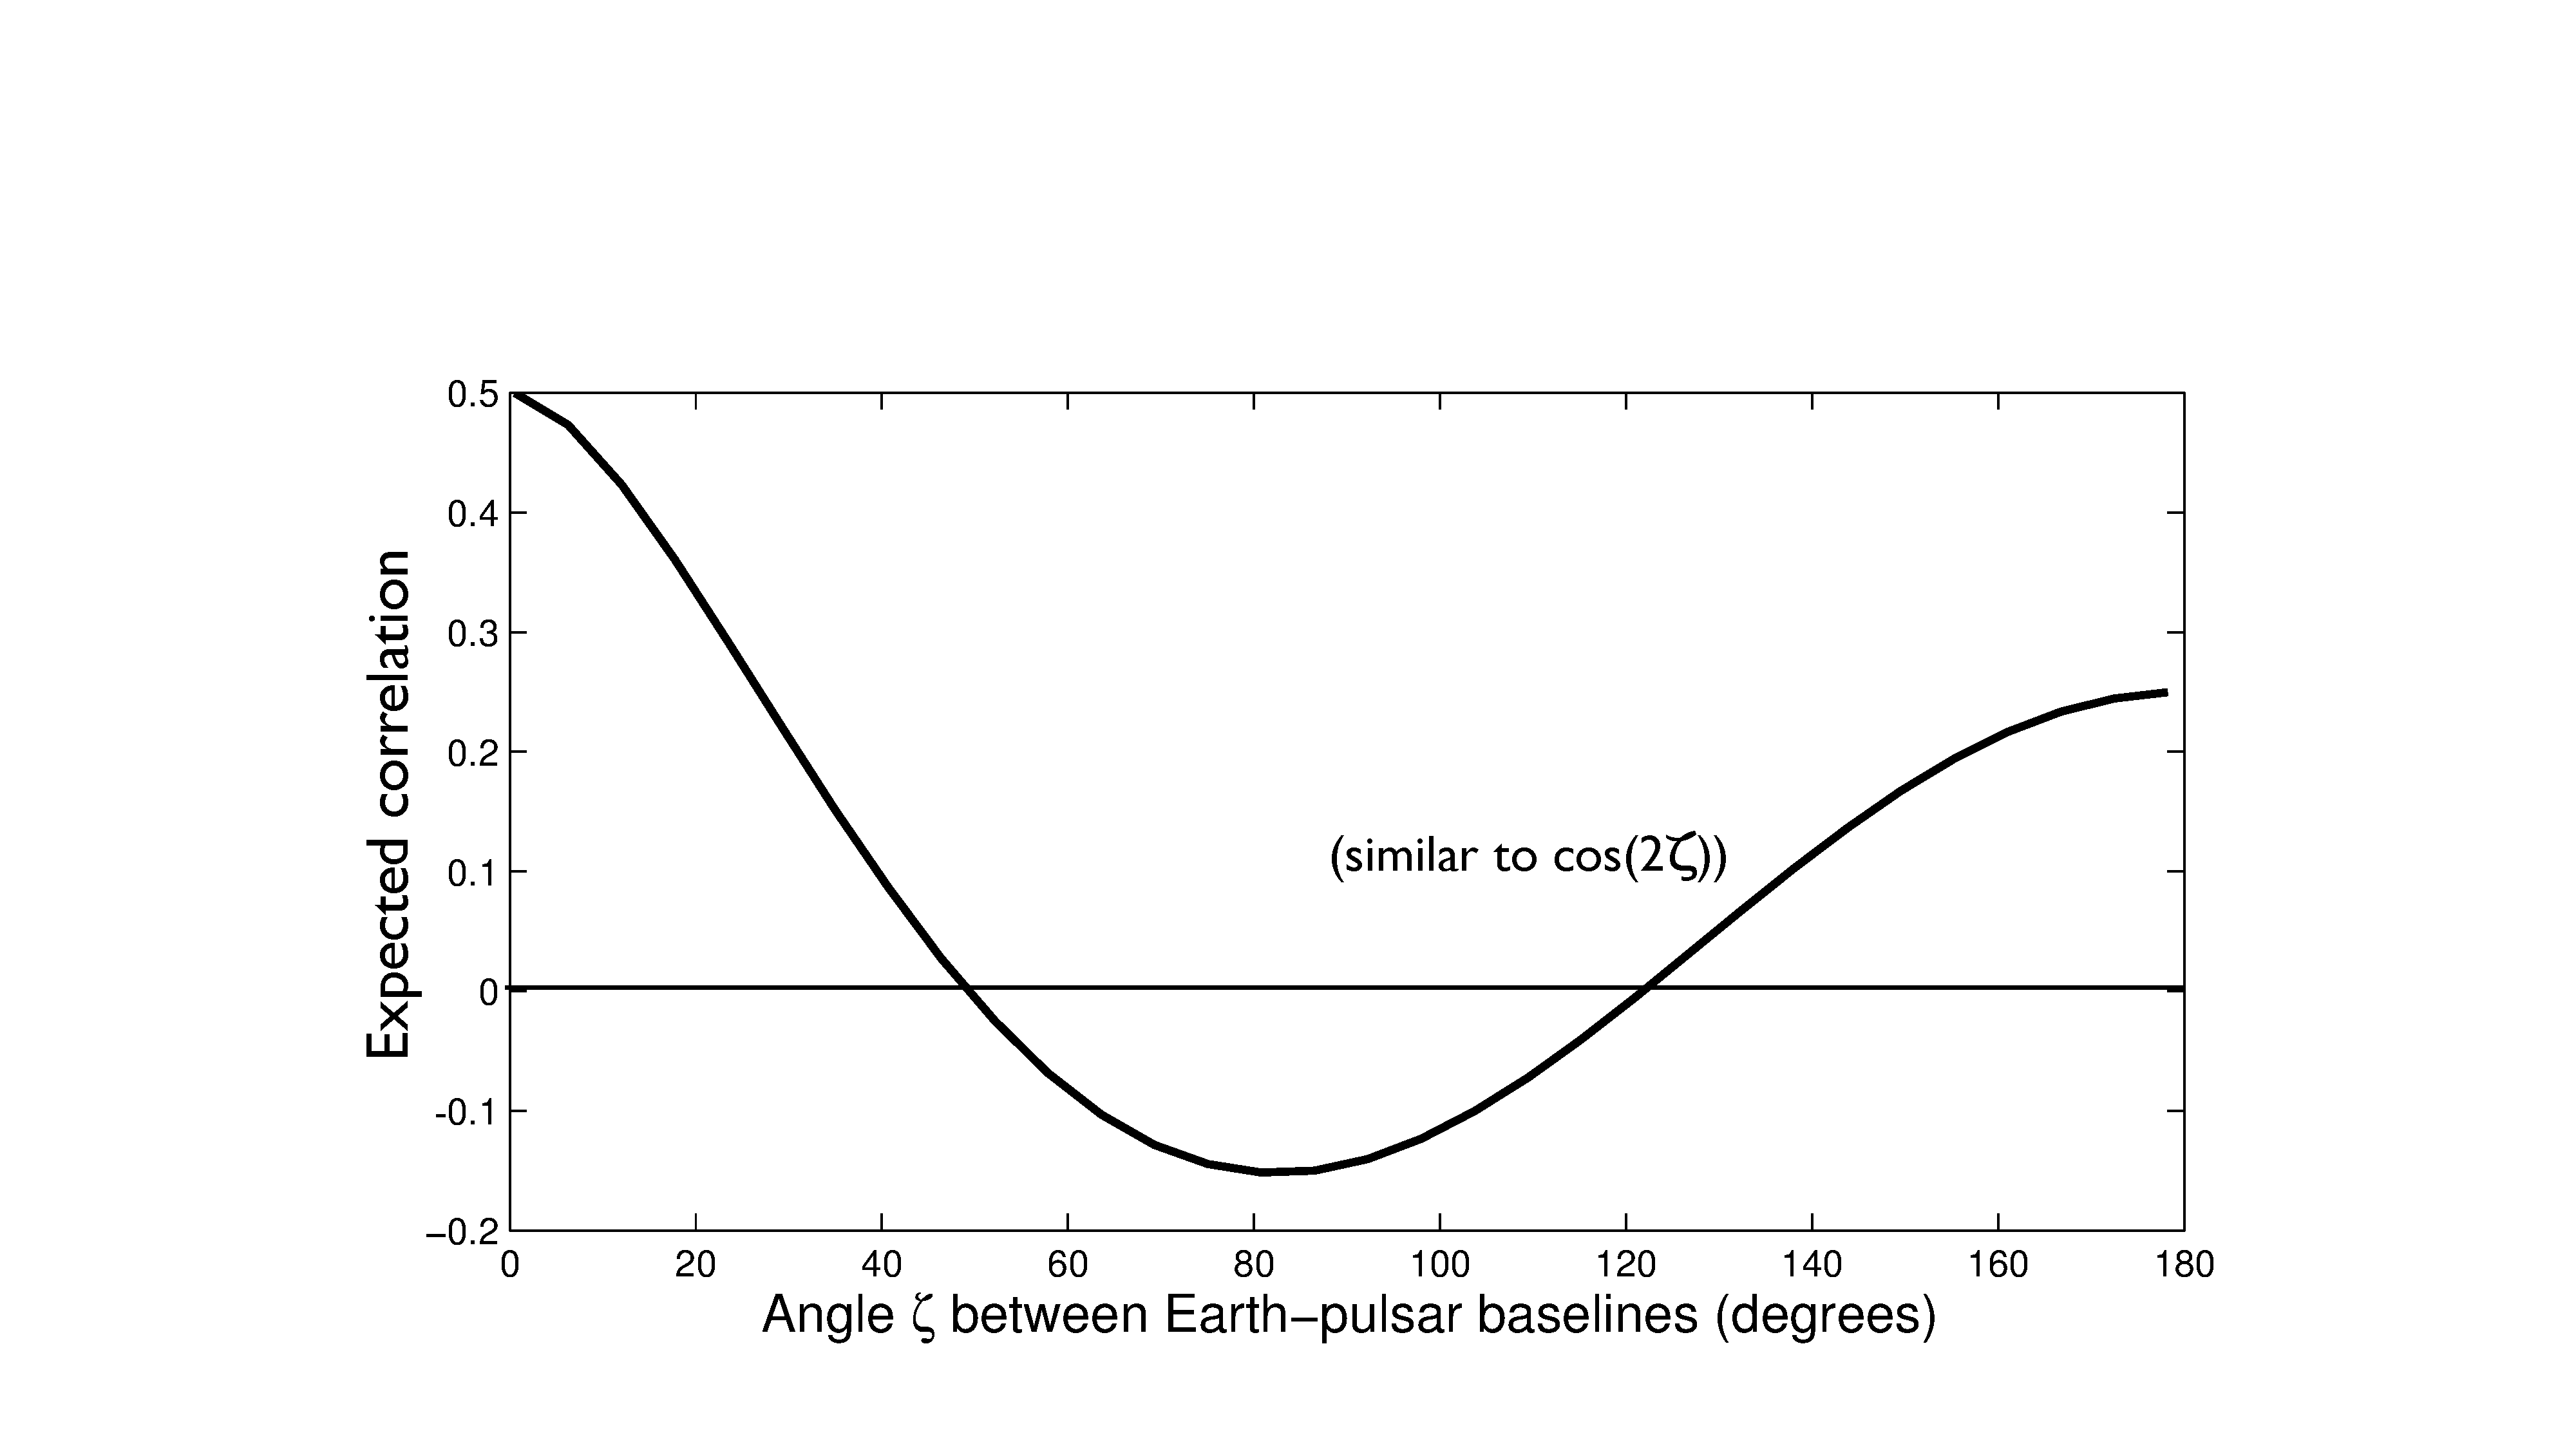
\includegraphics[width=0.7\textwidth]{Figures/HD_curve}
\caption{Hellings-Down curve.
The values of the expected correlation for an unpolarized,
isotropic GWB as a function of the angle $\zeta$ between
two Earth-pulsar baselines.}
\label{f:HD_curve}
\end{center}
\end{figure}

\begin{figure}[htbp!]
\begin{center}
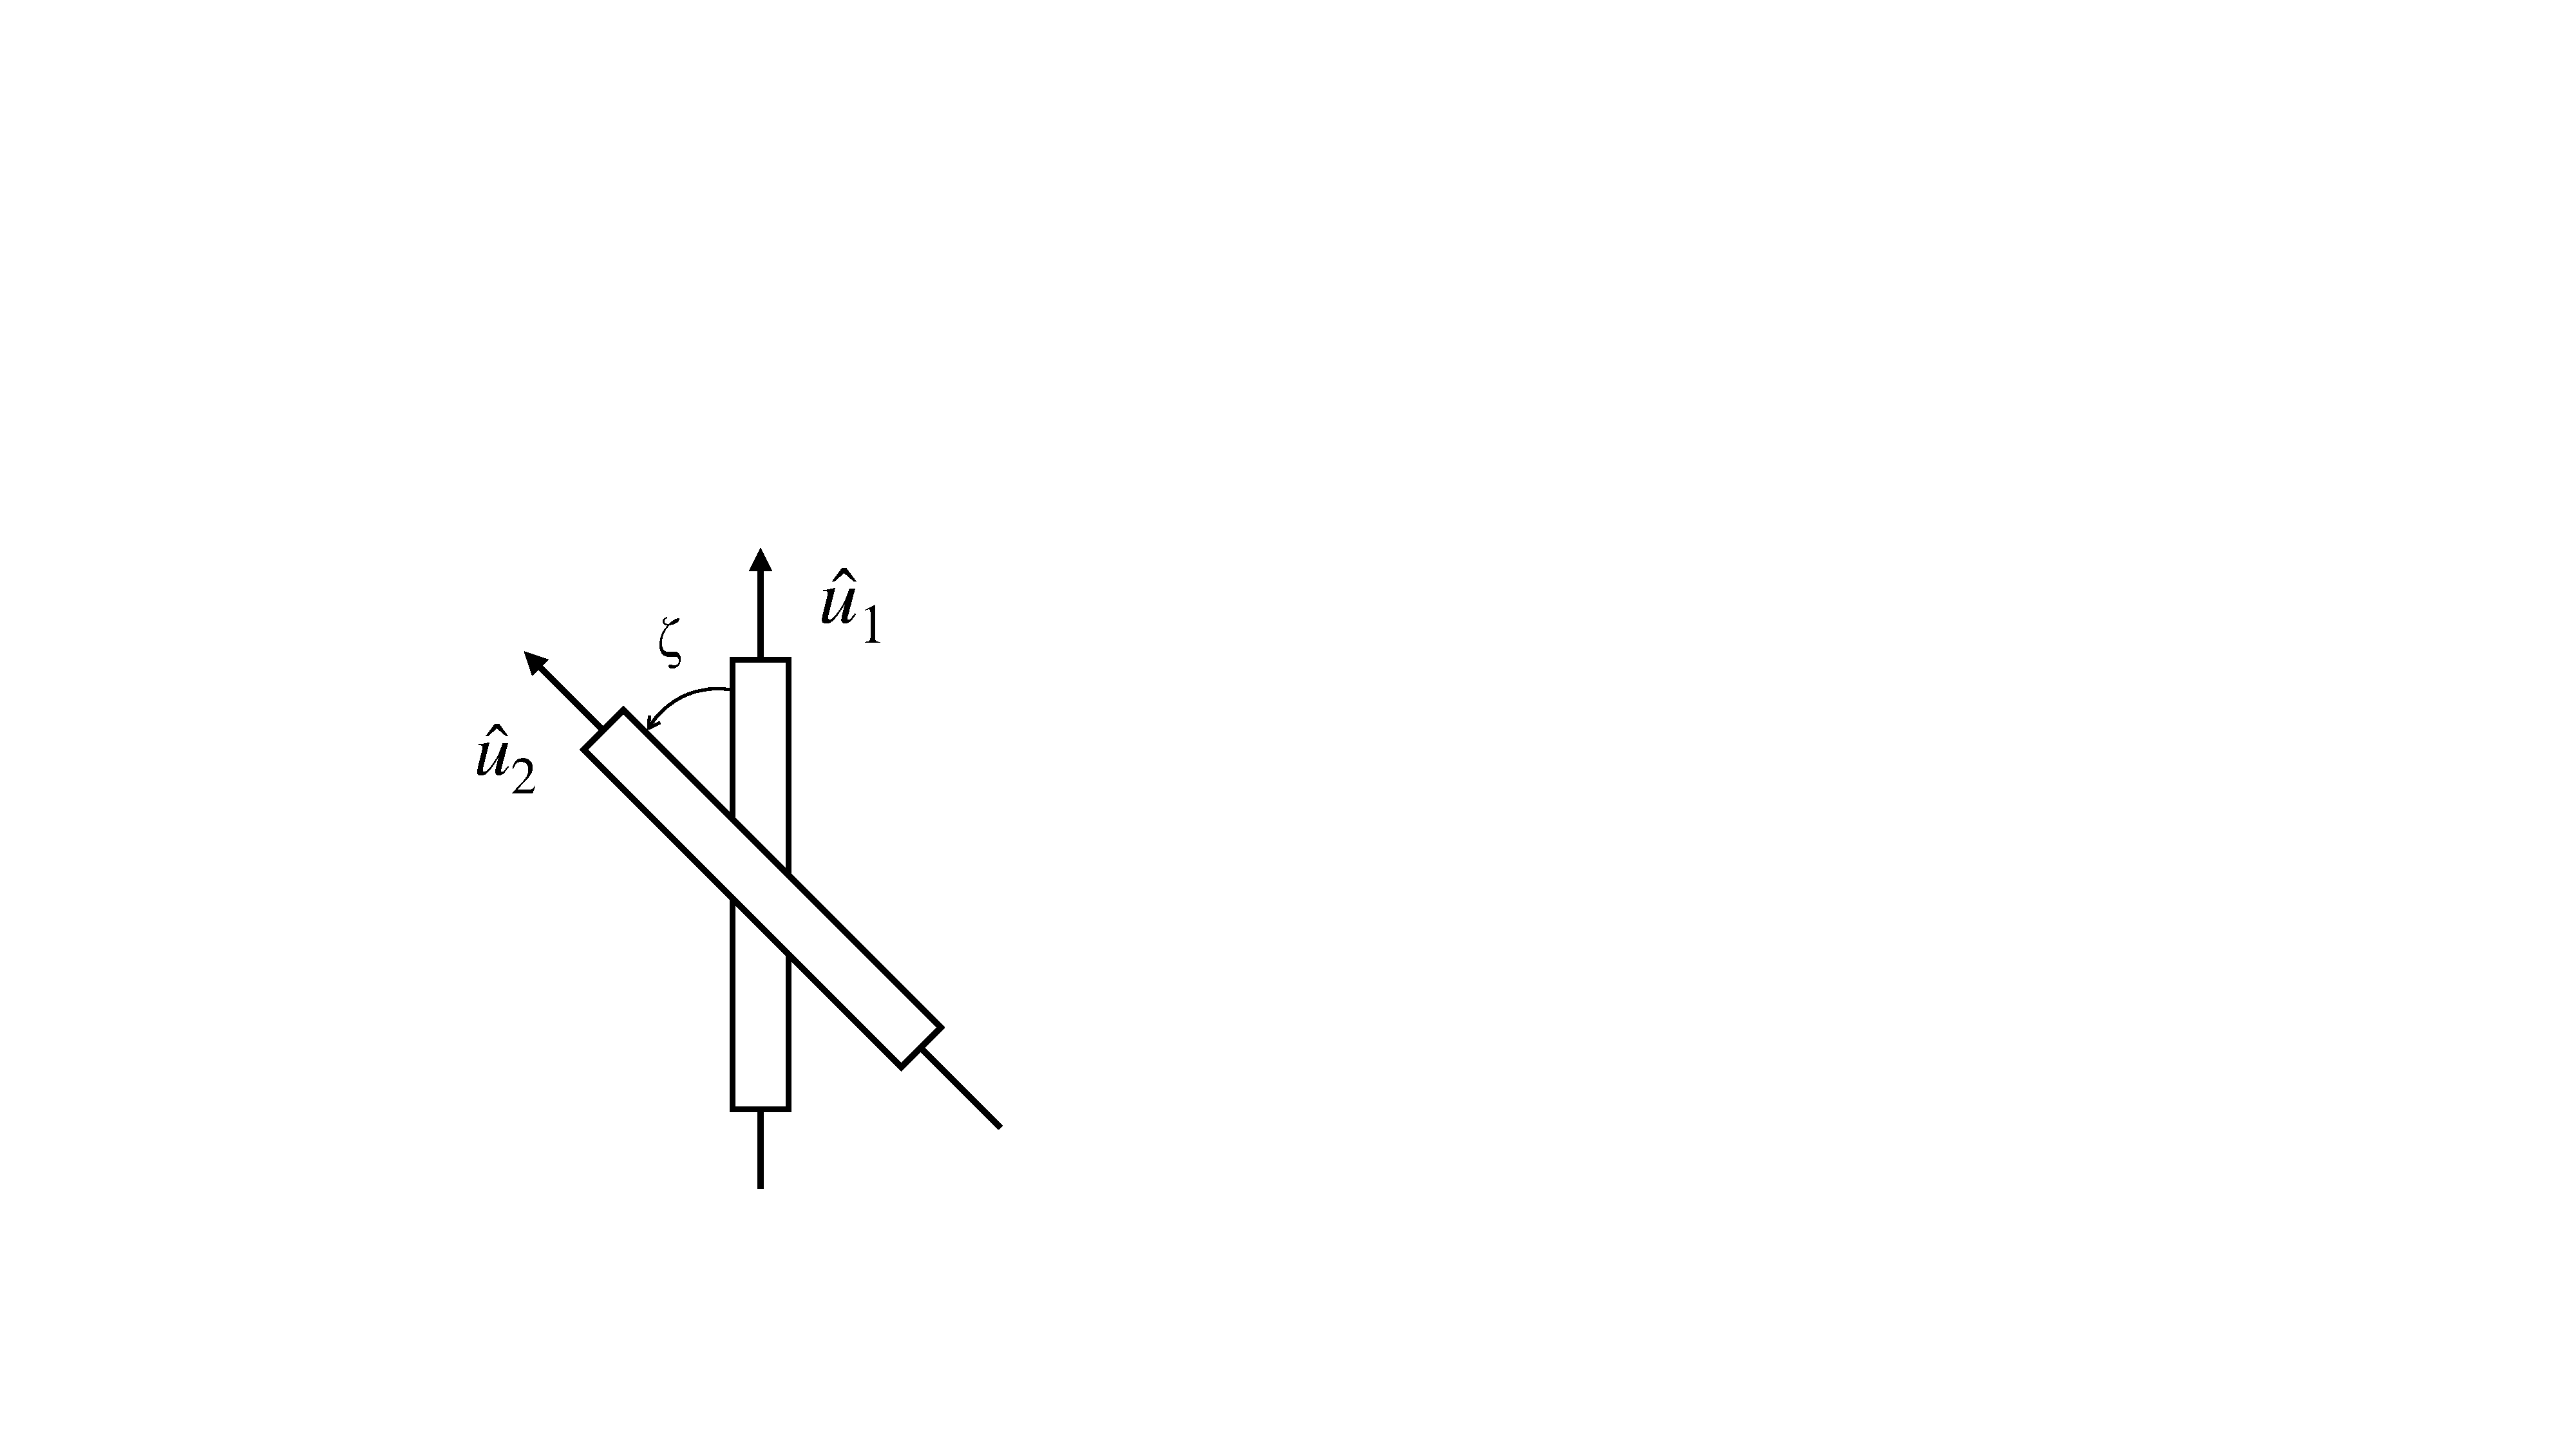
\includegraphics[width=0.25\textwidth]{Figures/dipole-orf}
\caption{Geometry for calculating the overlap function
for a pair of short, electric dipole antennae, for an
unpolarized and isotropic electric field
(Exercise 7).}
\label{f:dipole-orf}
\end{center}
\end{figure}

%%%%%%%%%%%%%%%%%%%%%%%%%%%%%%%%%%%%%%%%%%%%%%%%%%%%%%%
\section{What to do in the absence of correlations?}

\begin{figure}[htbp!]
\begin{center}
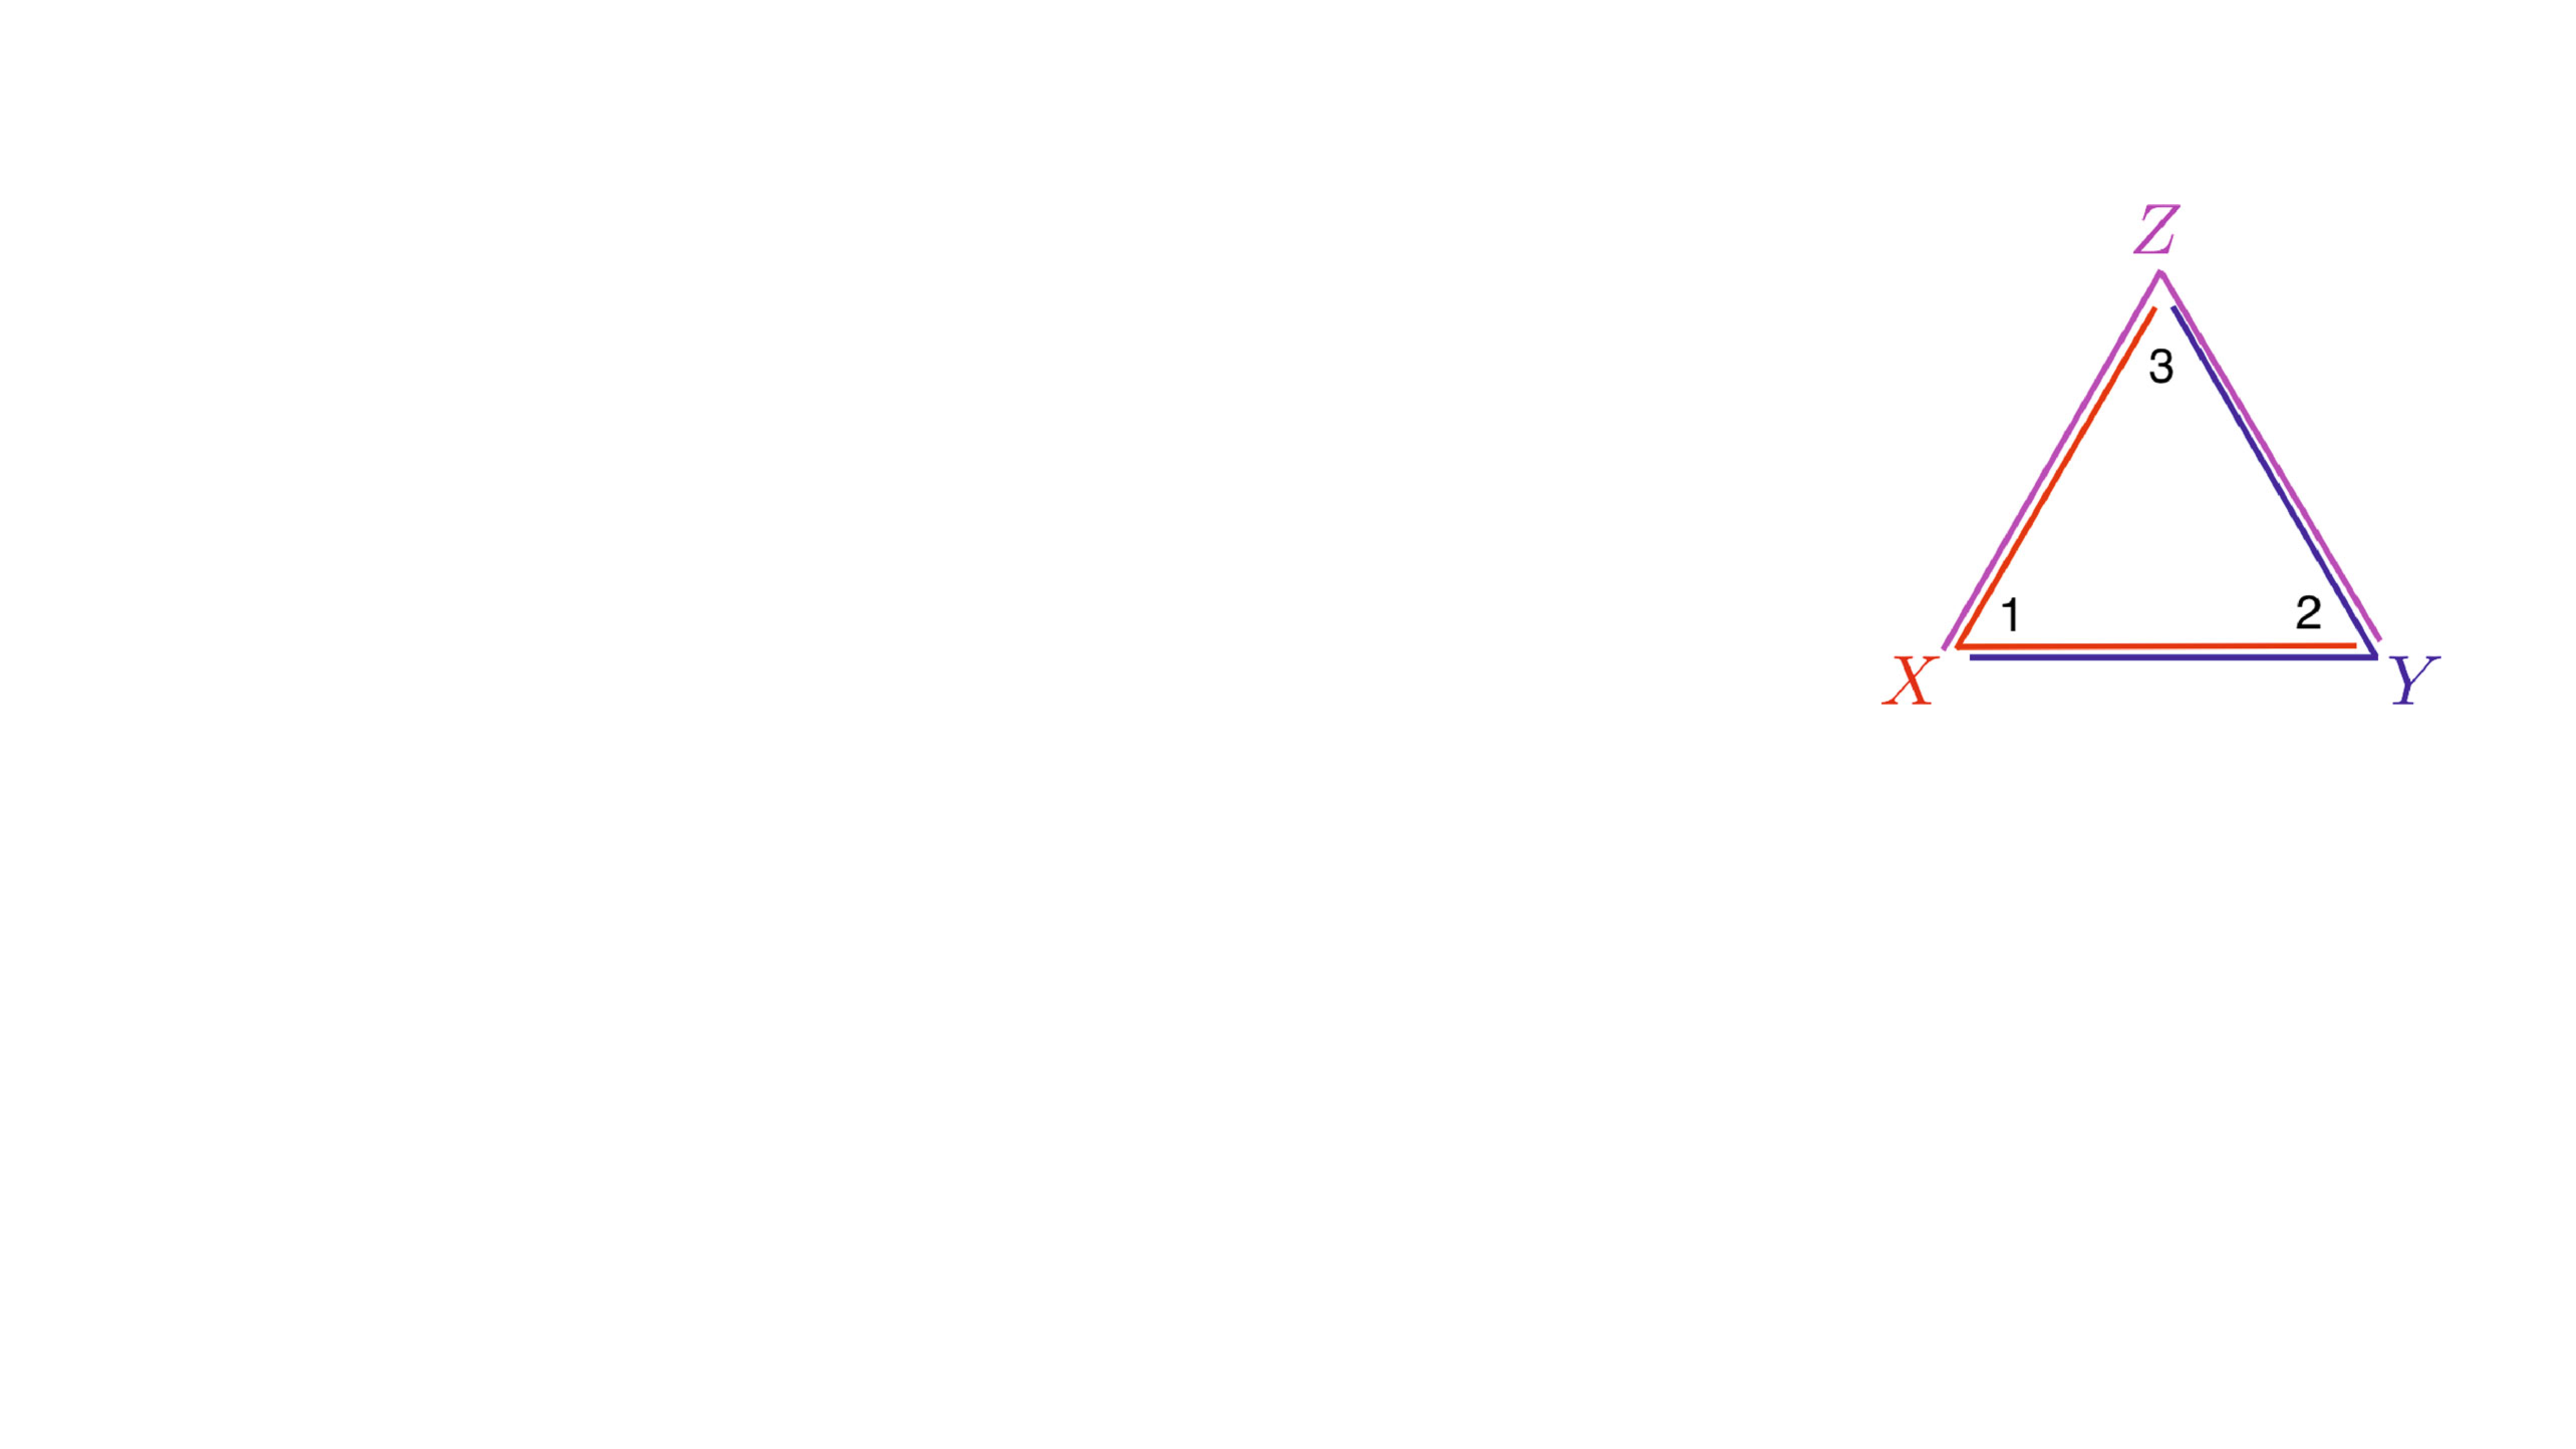
\includegraphics[width=0.3\textwidth]{Figures/LISA_XYZ}
\caption{Schematic representation of the LISA consellation.
$X$, $Y$, $Z$ correspond to Michelson interferometers 
with $60^\circ$ opening angles between the arms, with vertices
located at spacecraft 1, 2, 3.
From $X, Y, Z$, one can construct the TDI combinations
$A, E, T$ described in the text.}
\label{f:LISA_XYZ}
\end{center}
\end{figure}

\begin{figure}[htbp!]
\begin{center}
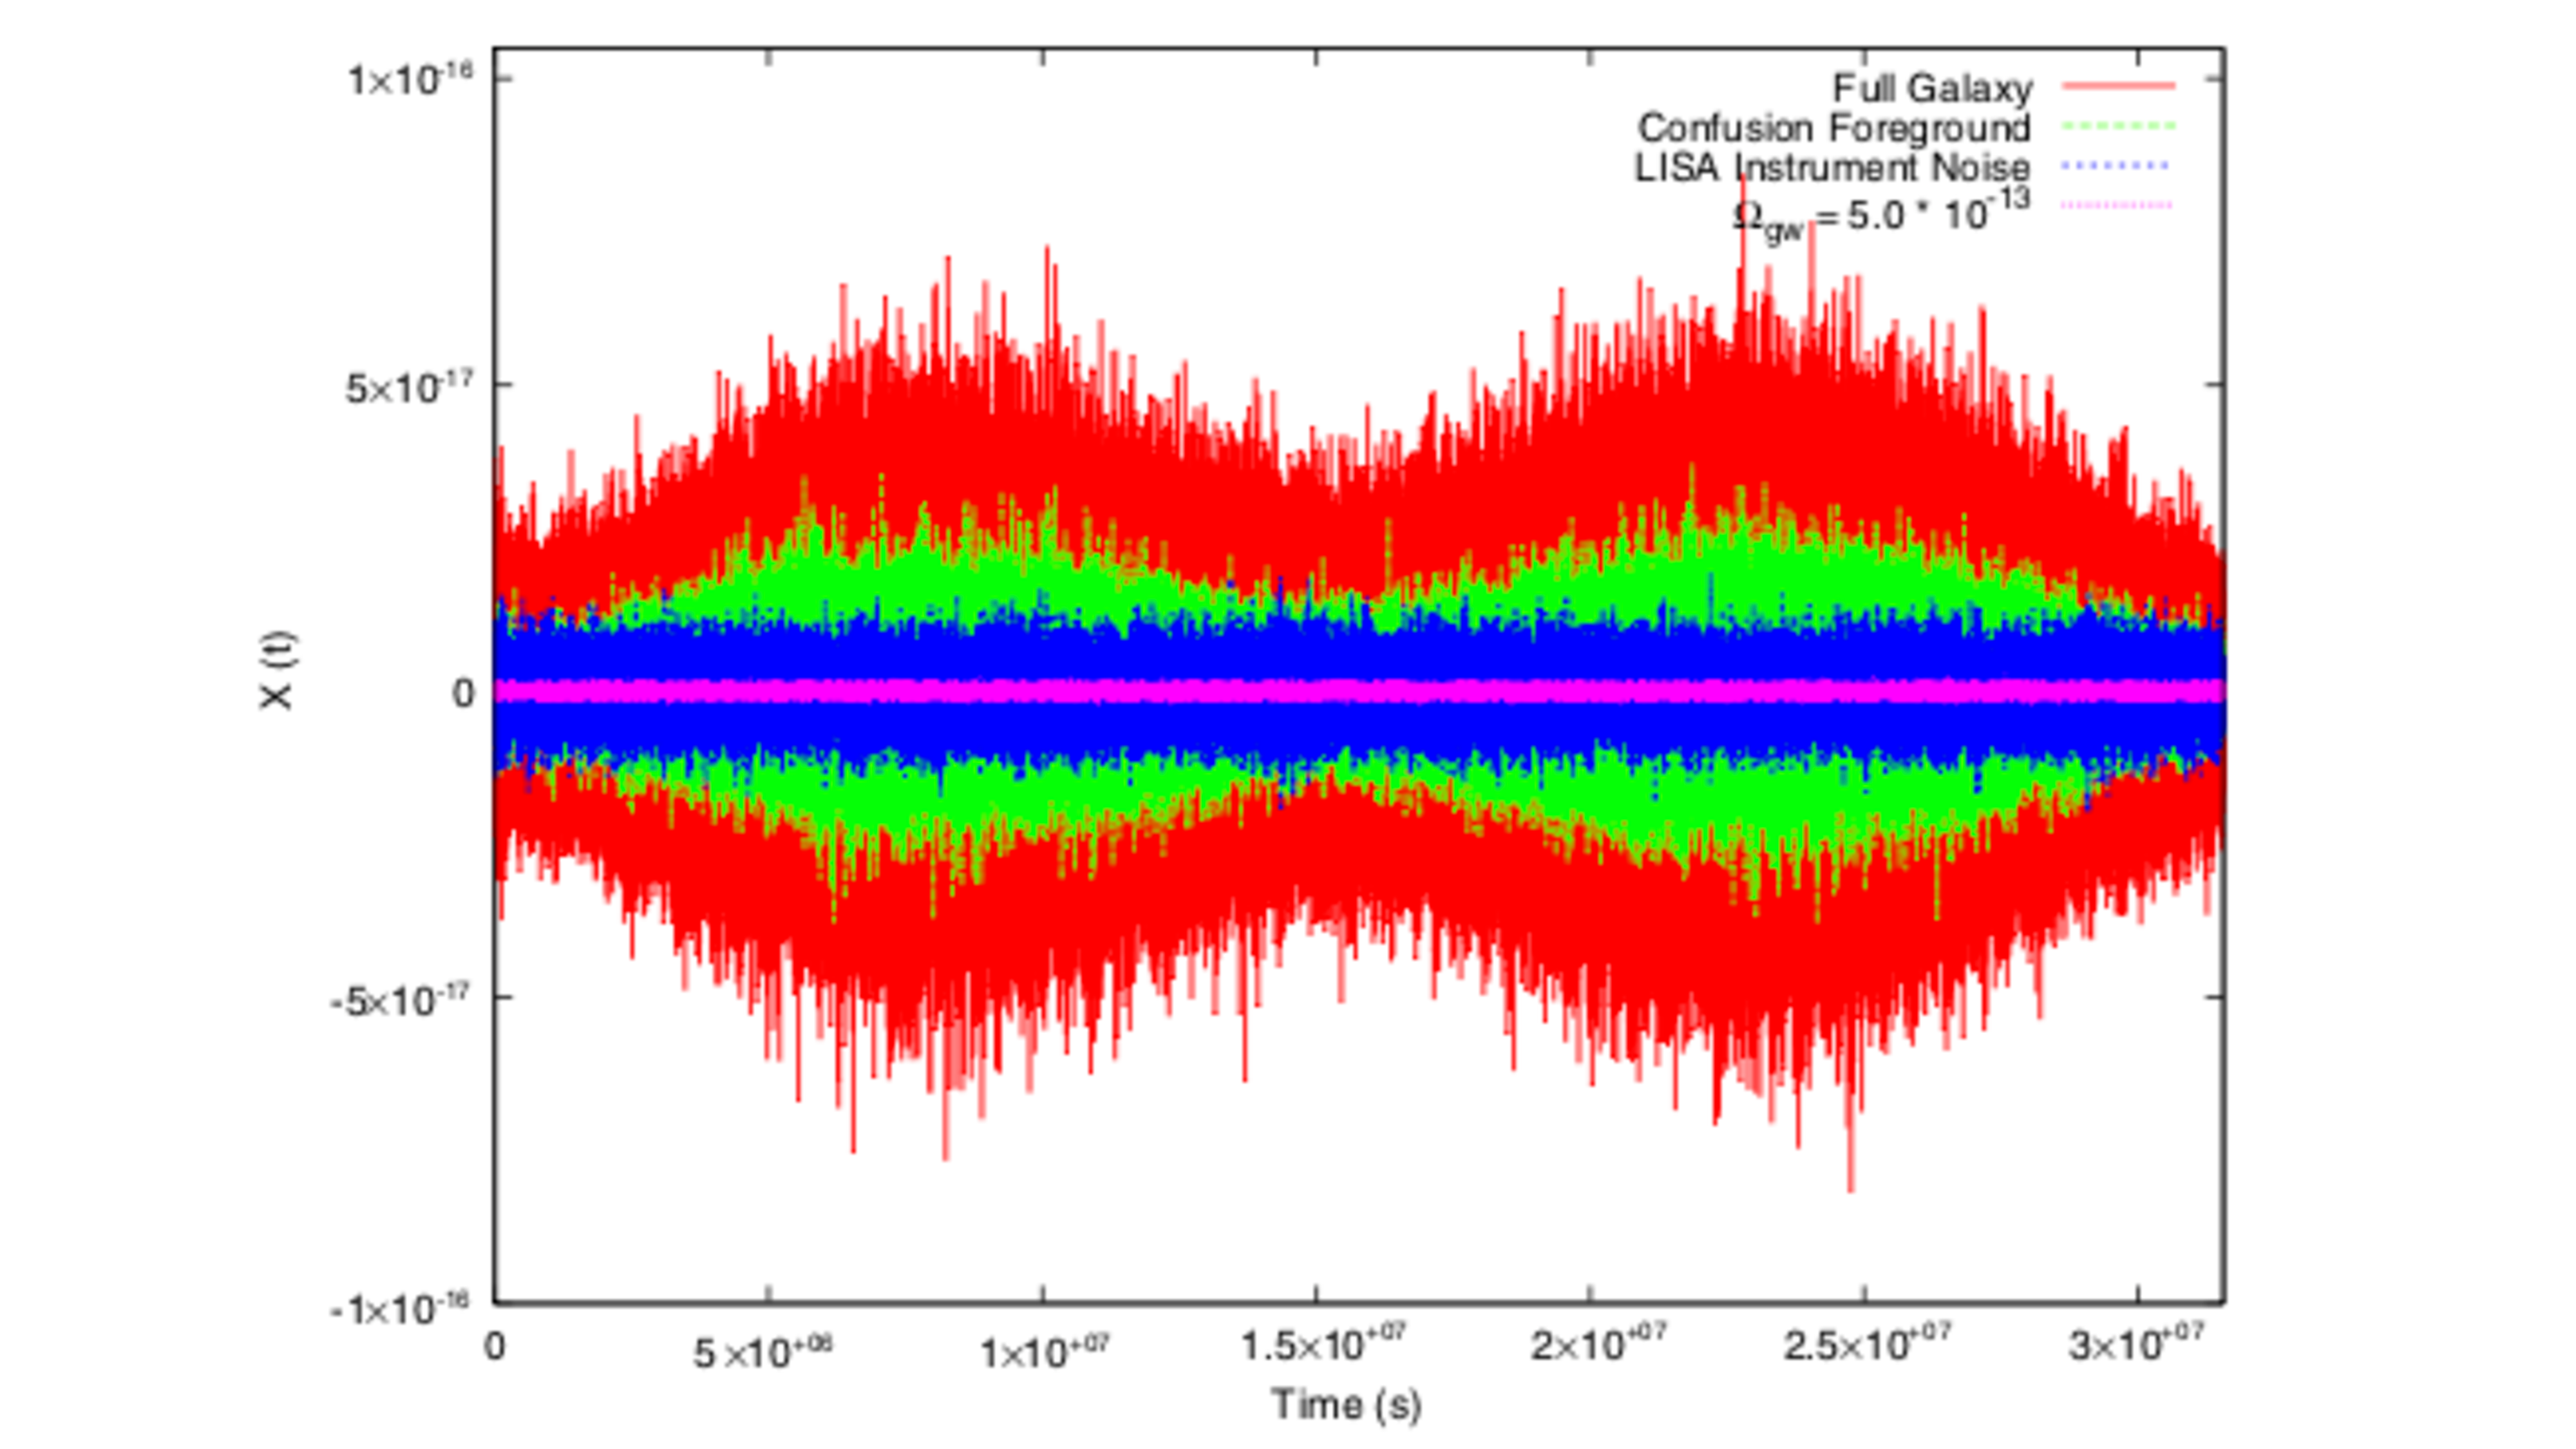
\includegraphics[width=0.7\textwidth]{Figures/LISA_timeseries}
\caption{One-years worth of simulated timeseries data for LISA.
The total output consists of a cosmological GWB (pink);
LISA instrument noise (blue); the full astrophysical foreground
signal from the galactic white-dwarf binary population (red),
which consist of individually resolvable binary signal and 
the confusion-limited foreground (green).
Of particular note are the amplitude and time variability 
of the astrophysical foreground, having a period of 6~months.
Figure taken from \cite{Adams-Cornish:2014}.}
\label{f:LISA_timeseries}
\end{center}
\end{figure}
\begin{figure}[htbp!]

\begin{center}
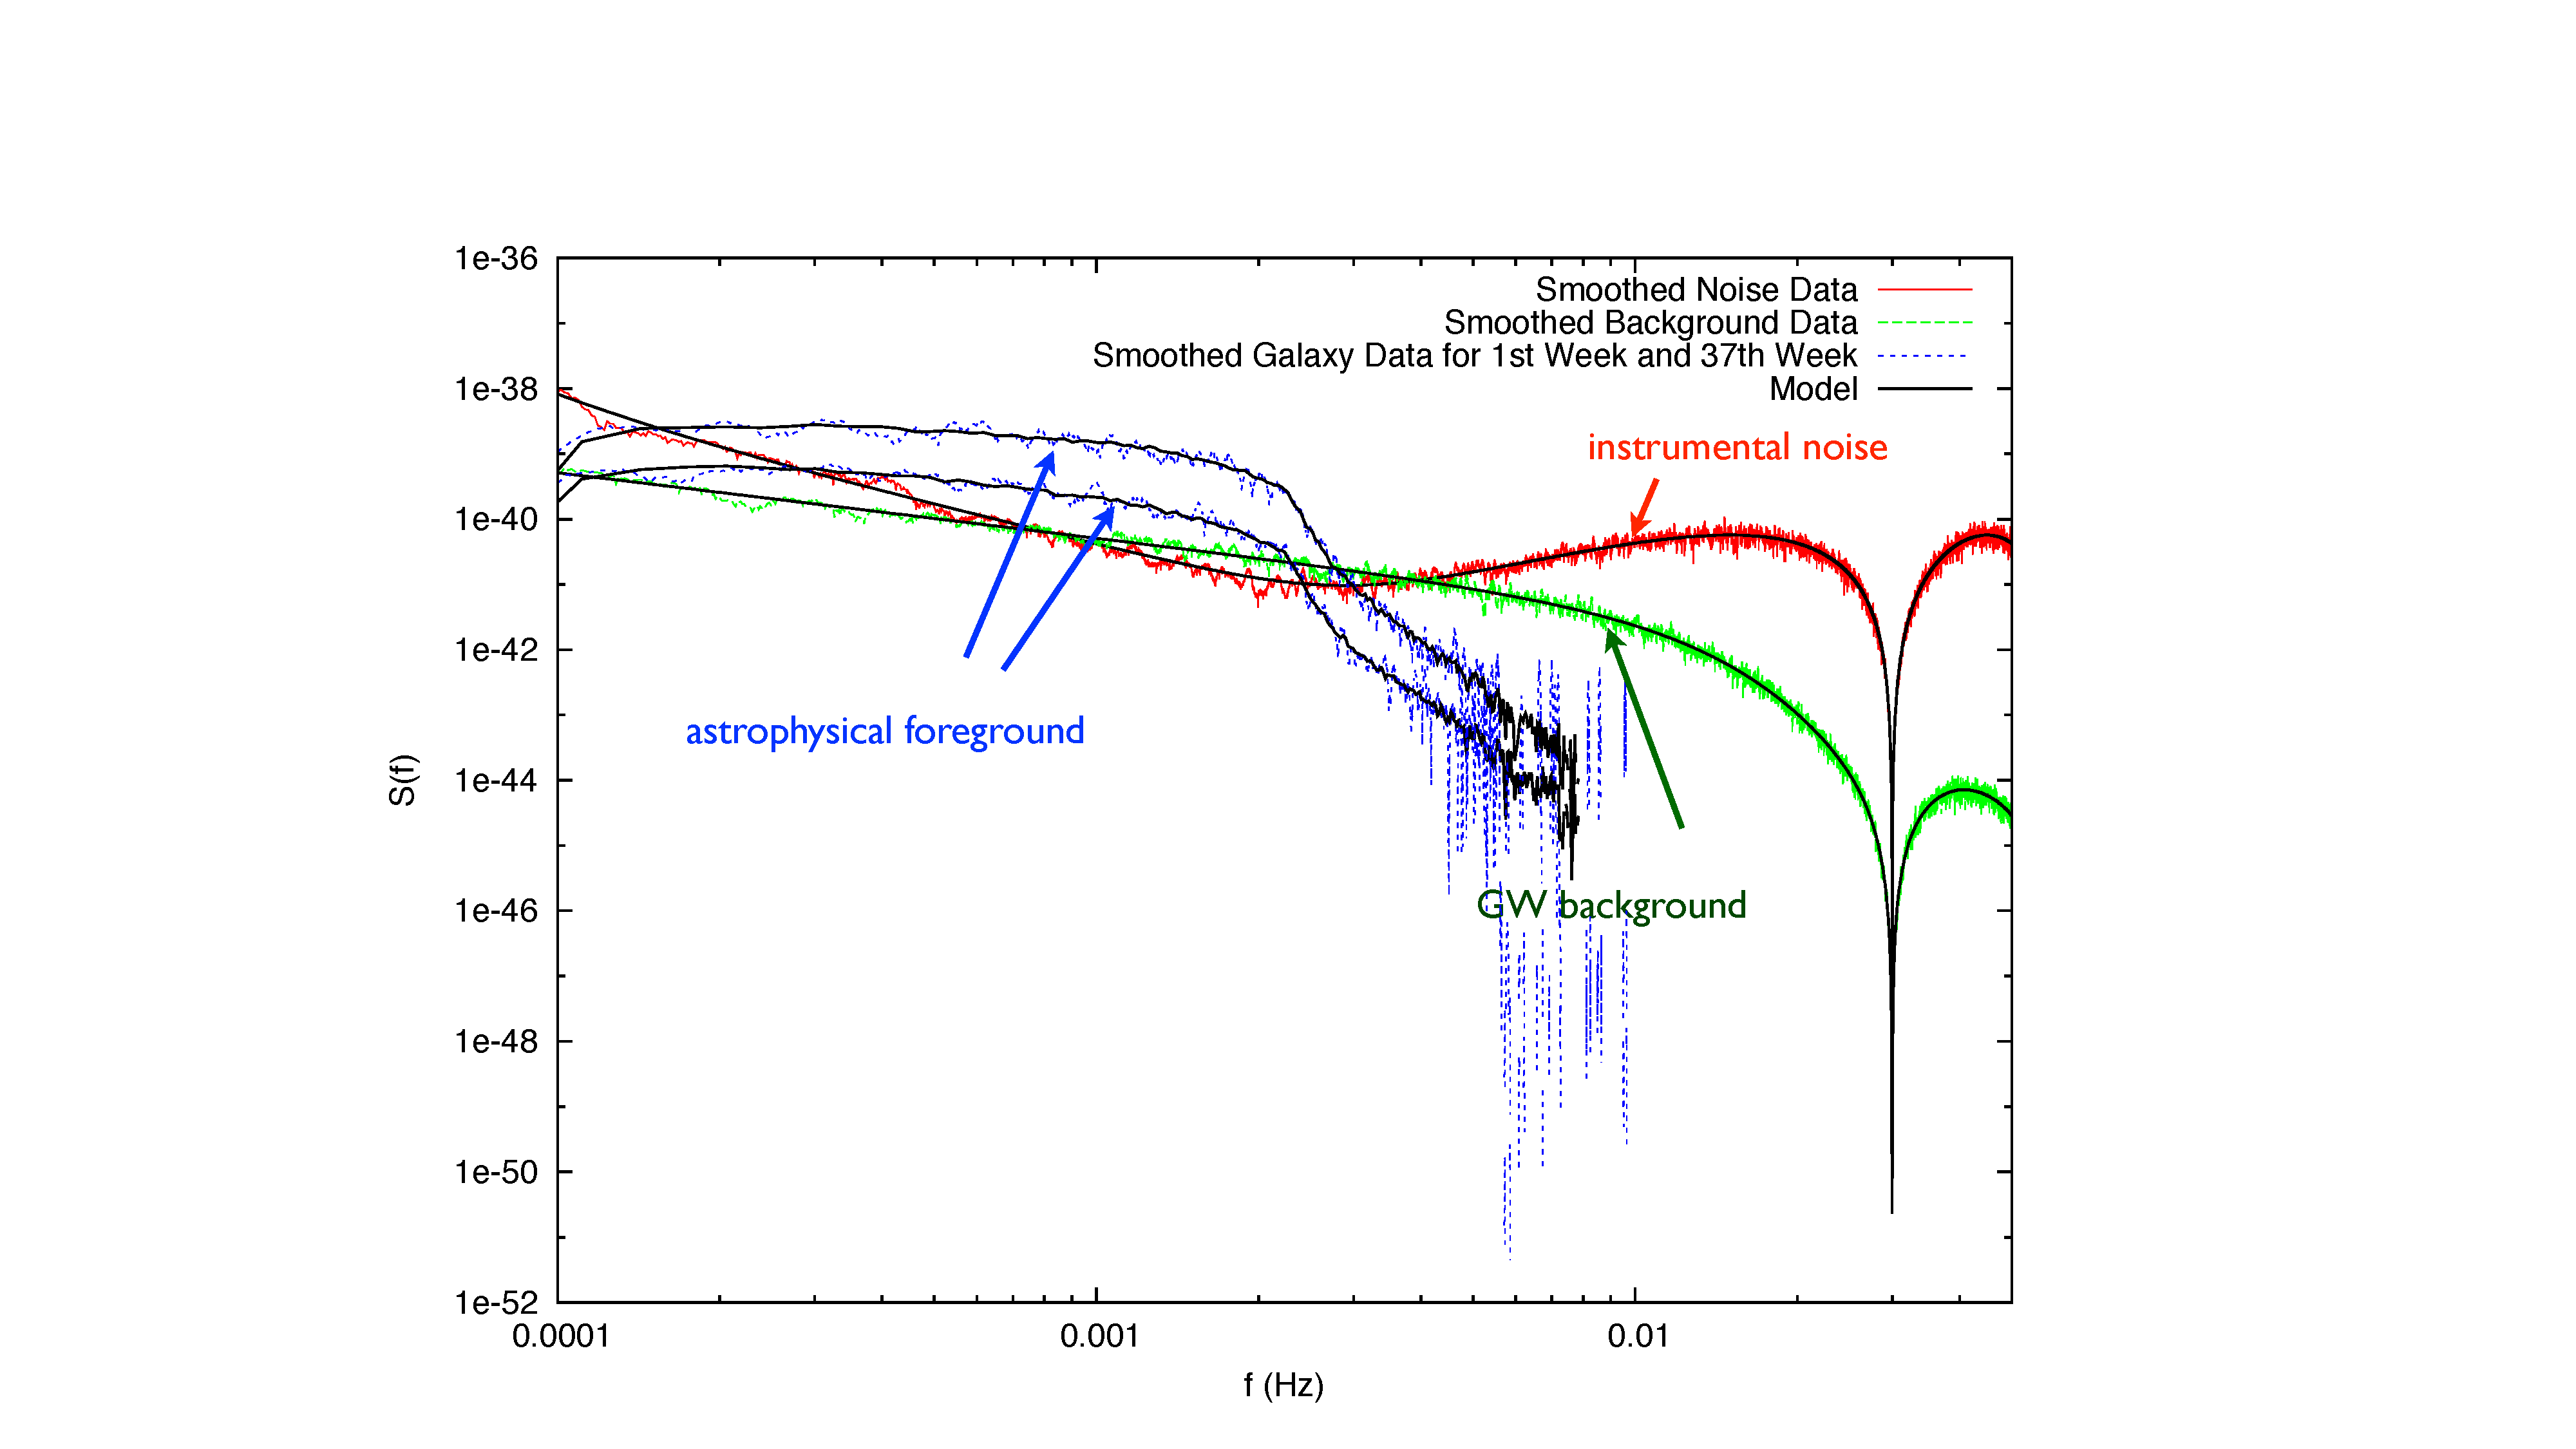
\includegraphics[width=0.6\textwidth]{Figures/LISA_psds}
\caption{Simulated power spectral densities for the 
LISA instrumental noise (red), cosmological GWB (green)
and astrophysical foreground from galactic white dwarf
binaries (blue), the latter at two times during LISAs orbit.
Note the strength of the astrophyical foreground relative
to the instrumental noise, and the different spectral shapes
for the three different contributions.
Figure taken from \cite{Adams-Cornish:2014}.}
\label{f:LISA_psds}
\end{center}
\end{figure}

%%%%%%%%%%%%%%%%%%%%%%%%%%%%%%%%%%%%%%%%%%%%%%%%%%%%%%%
\section{Frequentist statistics and Bayesian inference}

\begin{table}[tb]
\addtocounter{table}{-1}
\centering
\begin{longtable}{p{2.75in} | p{2.75in}}
\hline
FREQUENTIST STATISTICS & BAYESIAN INFERENCE\\
\hline
probabilities are long-run relative occurrence of 
outcomes of repeatable experiments (i.e., random variables);
cannot be assigned to hypotheses or parameters, 
which have fixed but unknown values
&
probabilities are degree of belief (or confidence)
in any proposition, and hence 
can be assigned to hypotheses and parameters
\\
\hline
Usually start with a likelihood function $p(d|H)$,
which is the probability distribution for the 
measured data $d$, assuming the truth of a particular
hypothesis $H$
&
same
\\
\hline
Construct statistics for parameter estimation and
hypothesis testing
&
Specify prior degree of belief for parameters and 
hypotheses
\\
\hline
Calculate the probability distribution of the 
statistic (e.g., using time slides)
&
Use Bayes' theorem to update degree of belief in
light of new data 
\\
\hline
constructs confidence intervals and $p$-values
&
constructs posteriors and odds ratios (Bayes factors)
\\
\hline
\end{longtable}
\vspace{0.2 in}
\caption{Comparison of frequentist and Bayesian approaches
to statistical inference.}
\label{t:bayesfreq}
\end{table}

\begin{figure}[htbp!]
\begin{center}
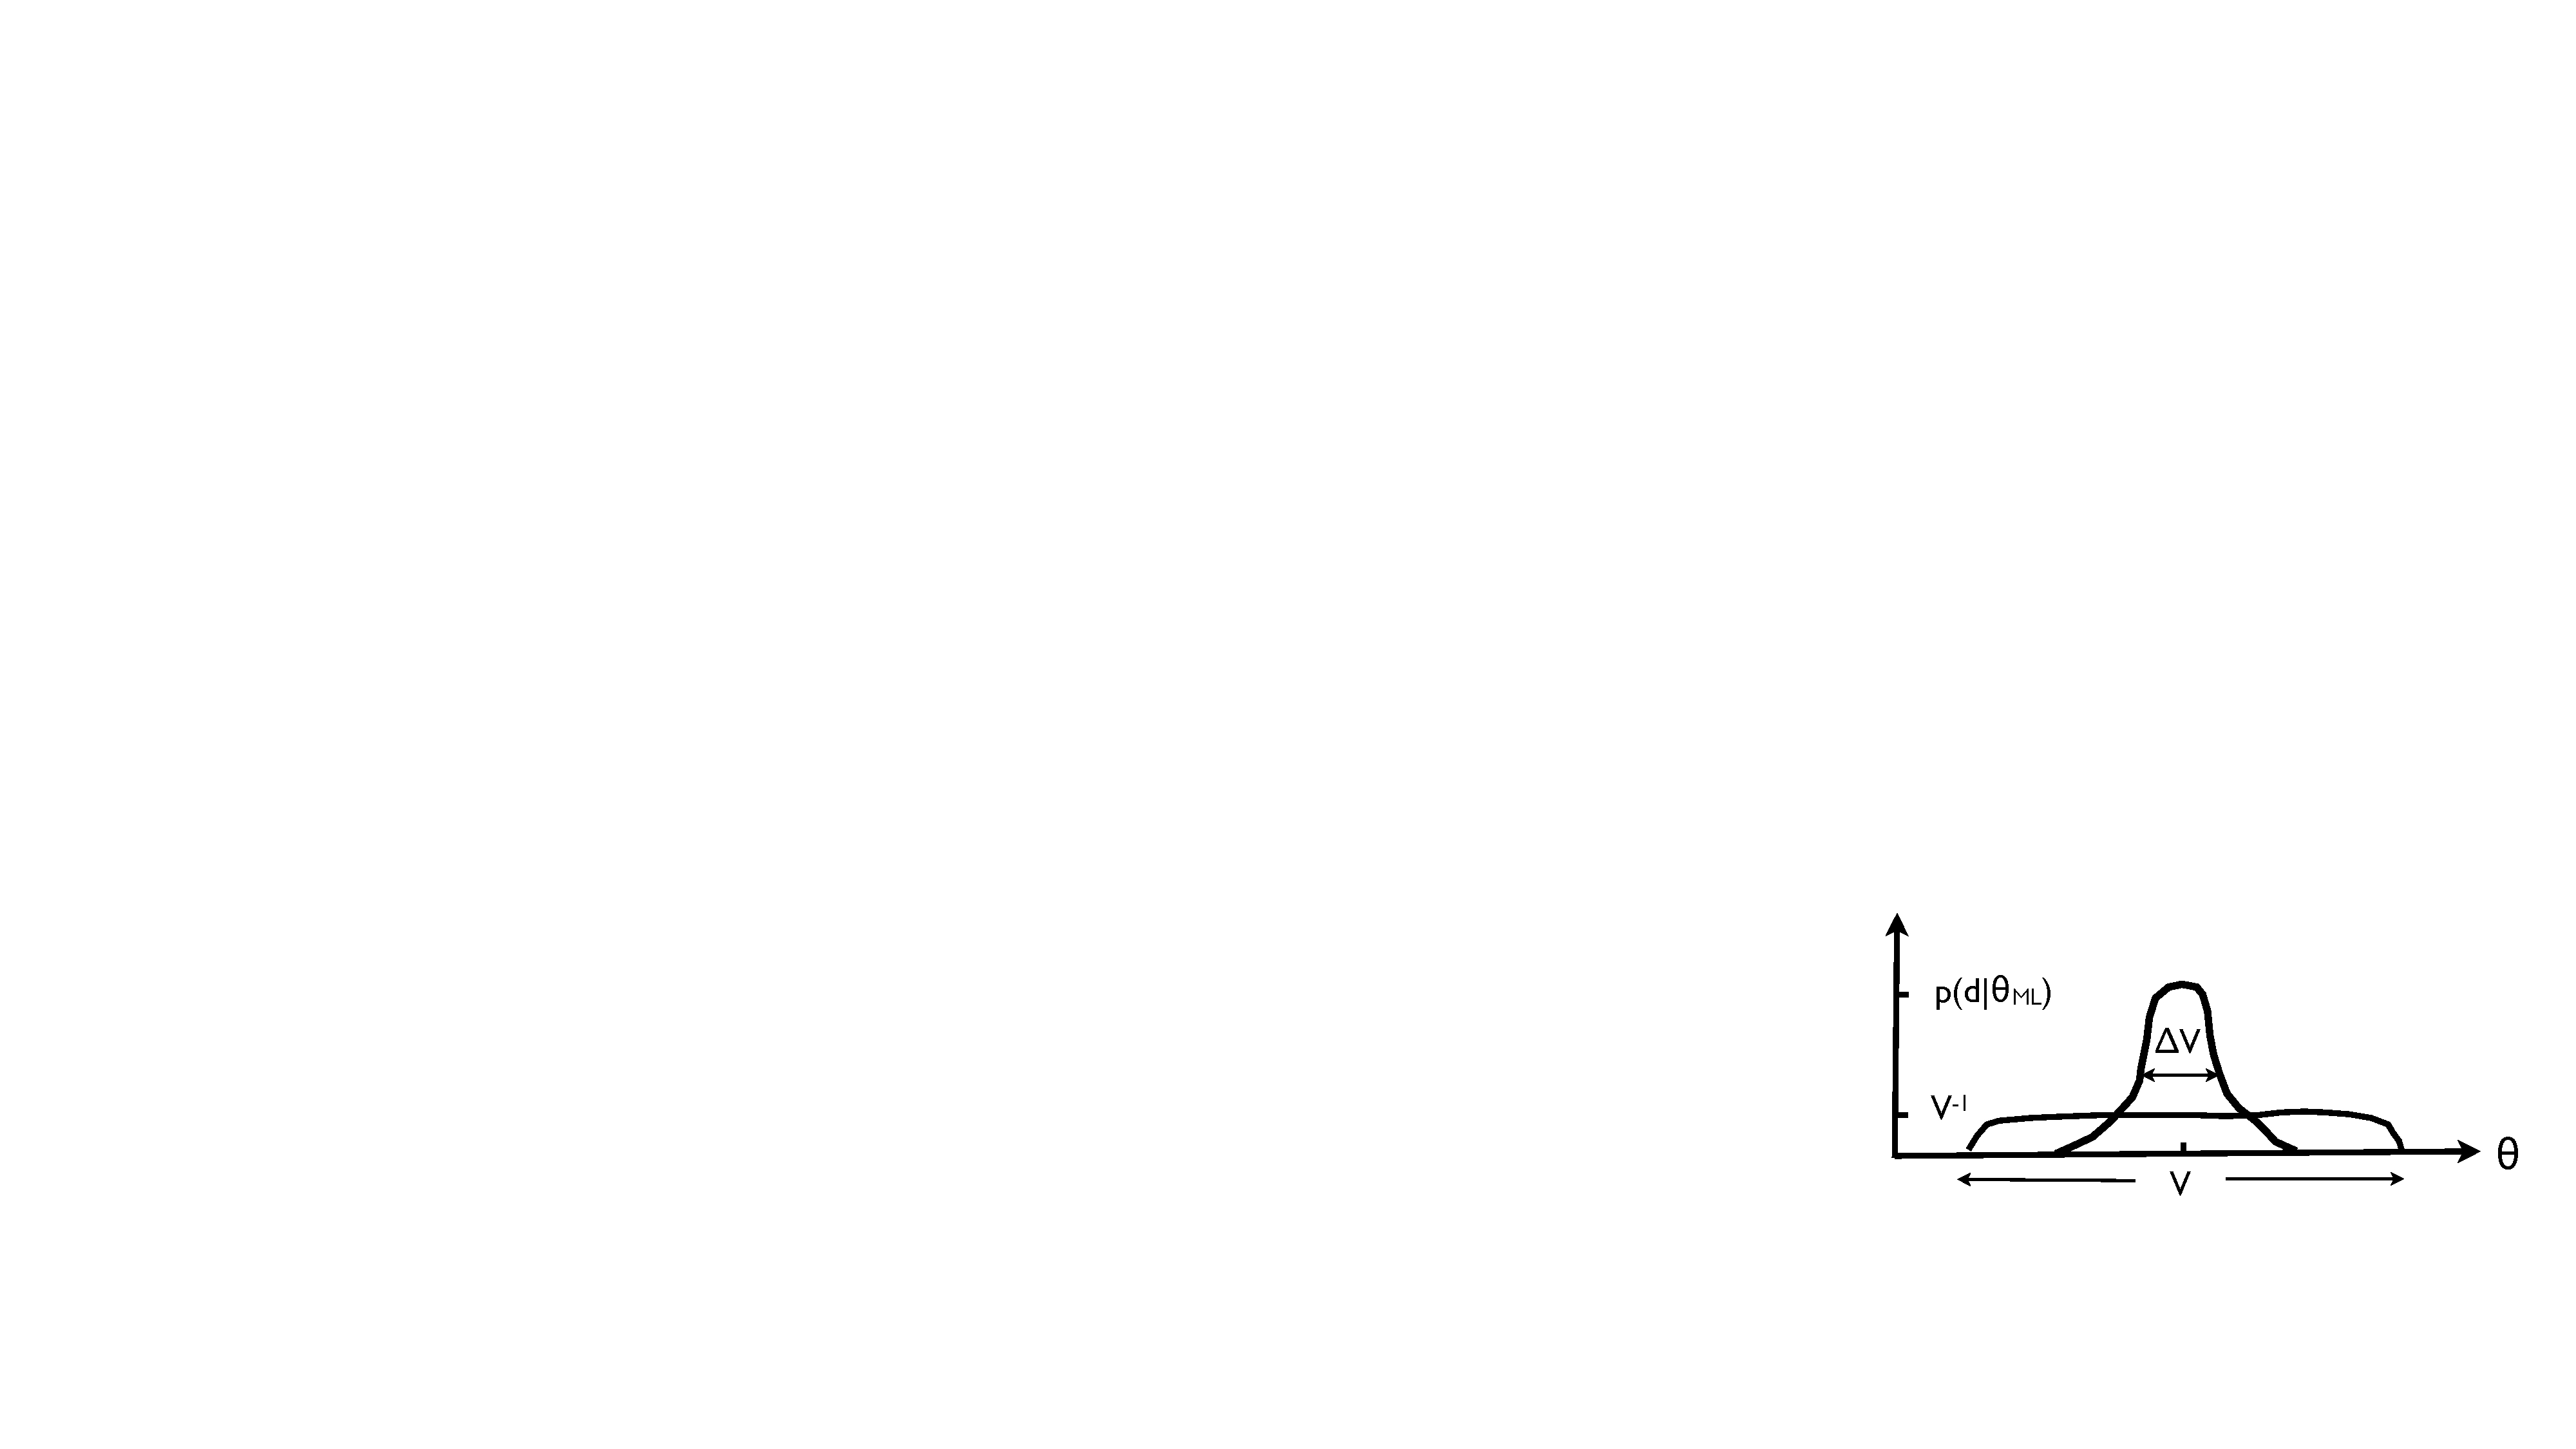
\includegraphics[width=0.45\textwidth]{Figures/informative_data}
\caption{Schematic representation of the likelihood function
and prior probability distribution for a parameter $\theta$,
when the data $d$ are informative.
In this case, thelikelihood function is peaked relative to the 
prior probability distribution, with maximum at 
$\theta=\theta_{\rm ML}$ and characteristic width $\Delta V$.
The parameter space volume is denoted by $V$.}
\label{f:informative_data}
\end{center}
\end{figure}

\begin{figure}[htbp!]
\begin{center}
\subfigure[]{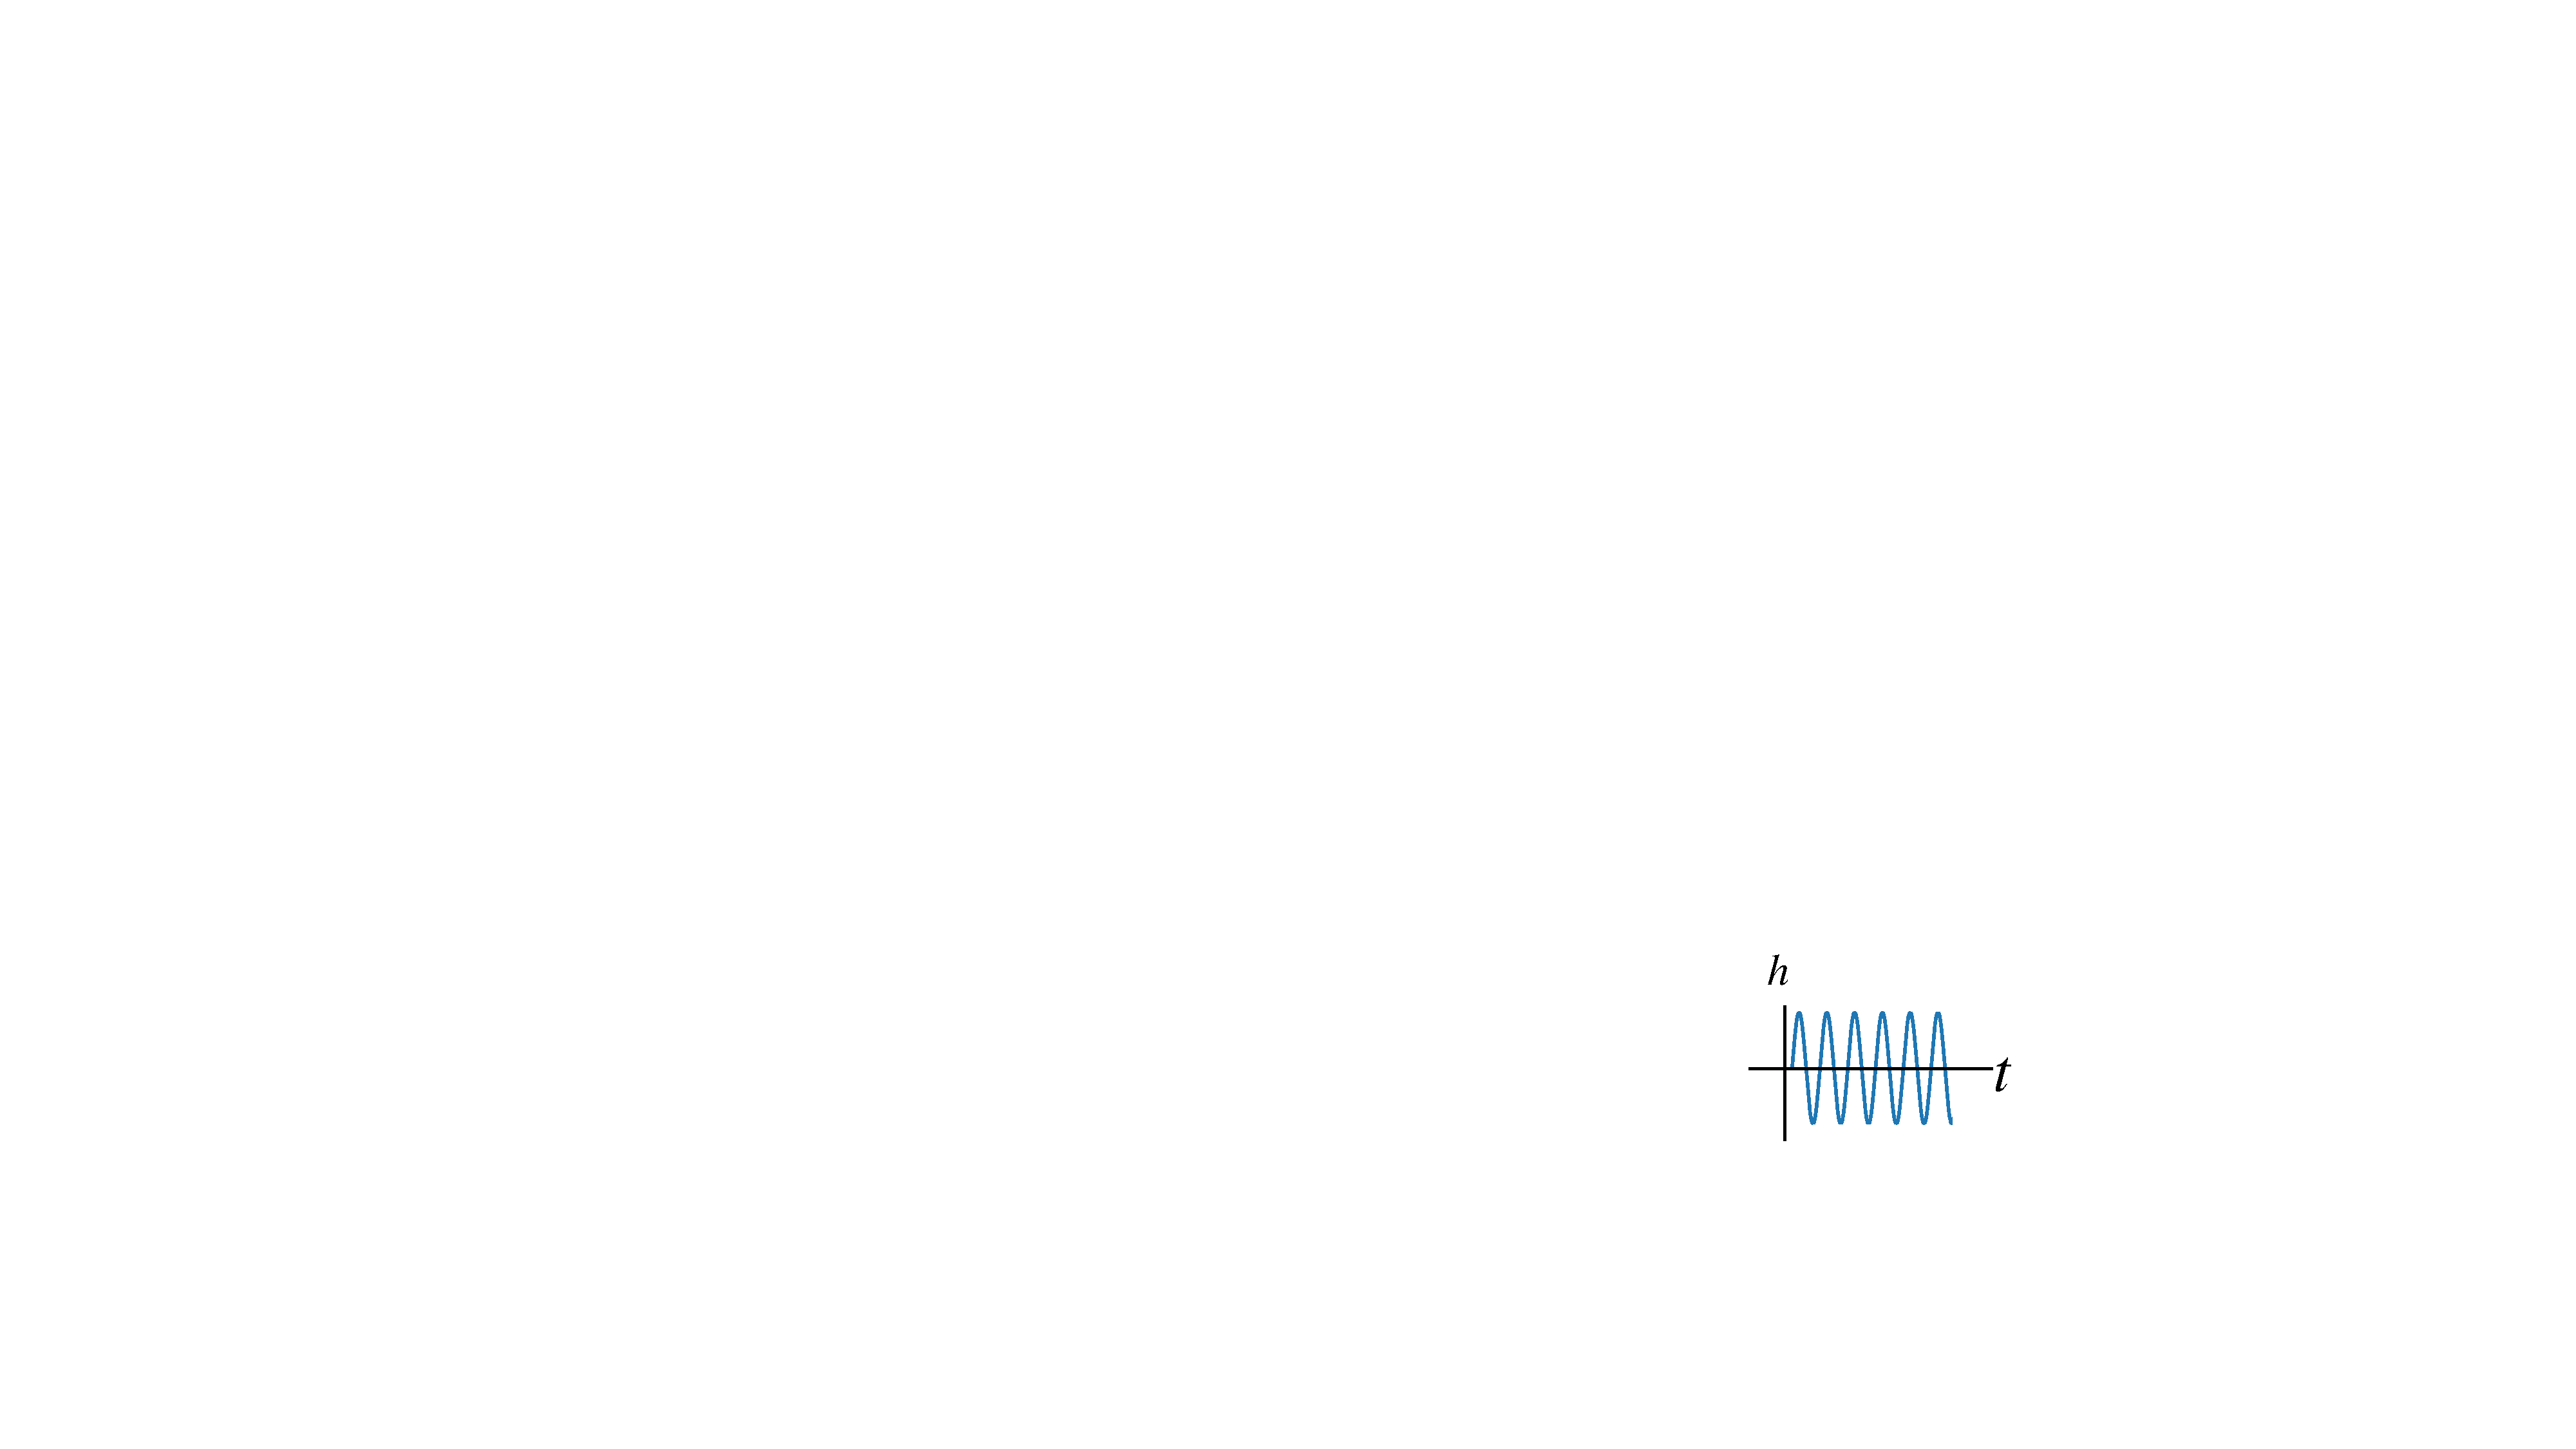
\includegraphics[width=0.25\textwidth]{Figures/sinusoid_prior}}
\hspace{1 in}
\subfigure[]{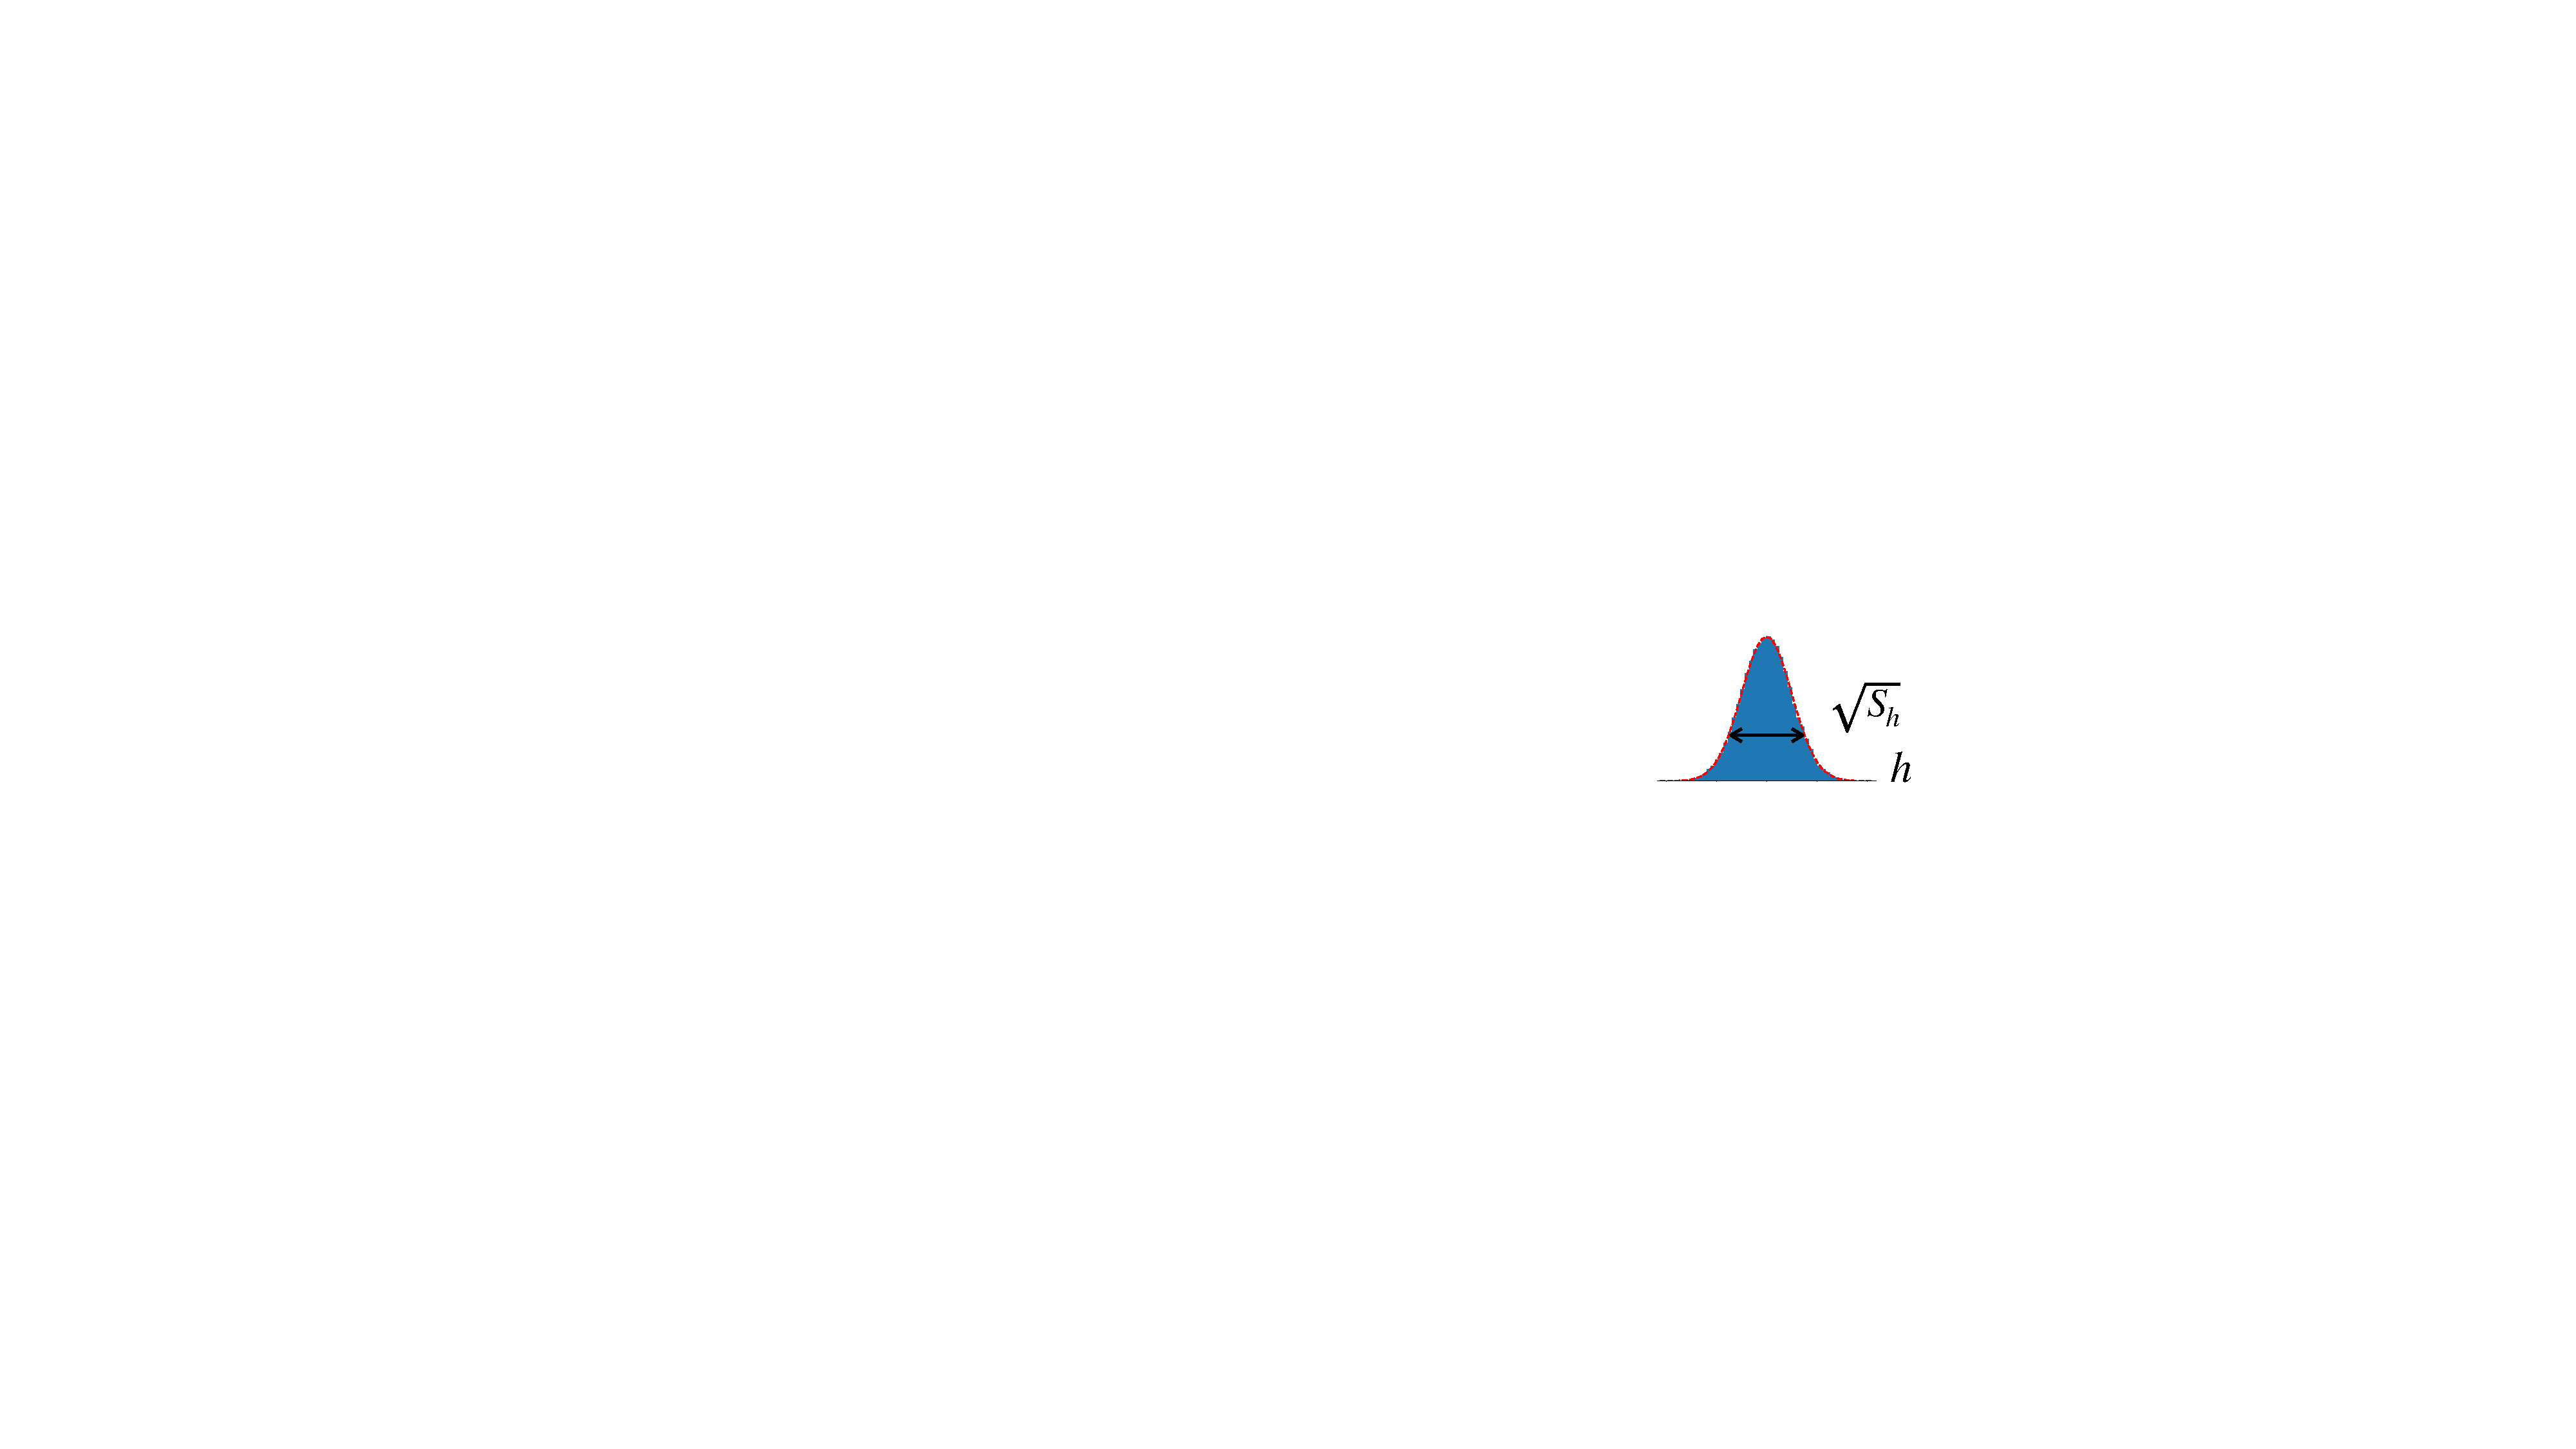
\includegraphics[width=0.25\textwidth]{Figures/stochastic_prior}}
\caption{Different signal priors for $h(t)$.
Panel (a): Determinsitic (sinusoid) signal prior.
Panel (b): Stochastic signal prior.
For the stochastic signal prior, $h(t)$ values are drawn from a
Gaussian distribution with variance $S_h$.}
\label{f:det_stoch_signal_priors}
\end{center}
\end{figure}

%%%%%%%%%%%%%%%%%%%%%%%%%%%%%%%%%%%%%%%%%%%%%%%%%%%%%%%
\section{Searching for the background of binary black-hole
mergers}
\label{s:nonstationary}

\begin{figure}[htbp!]
\begin{center}
\subfigure[]{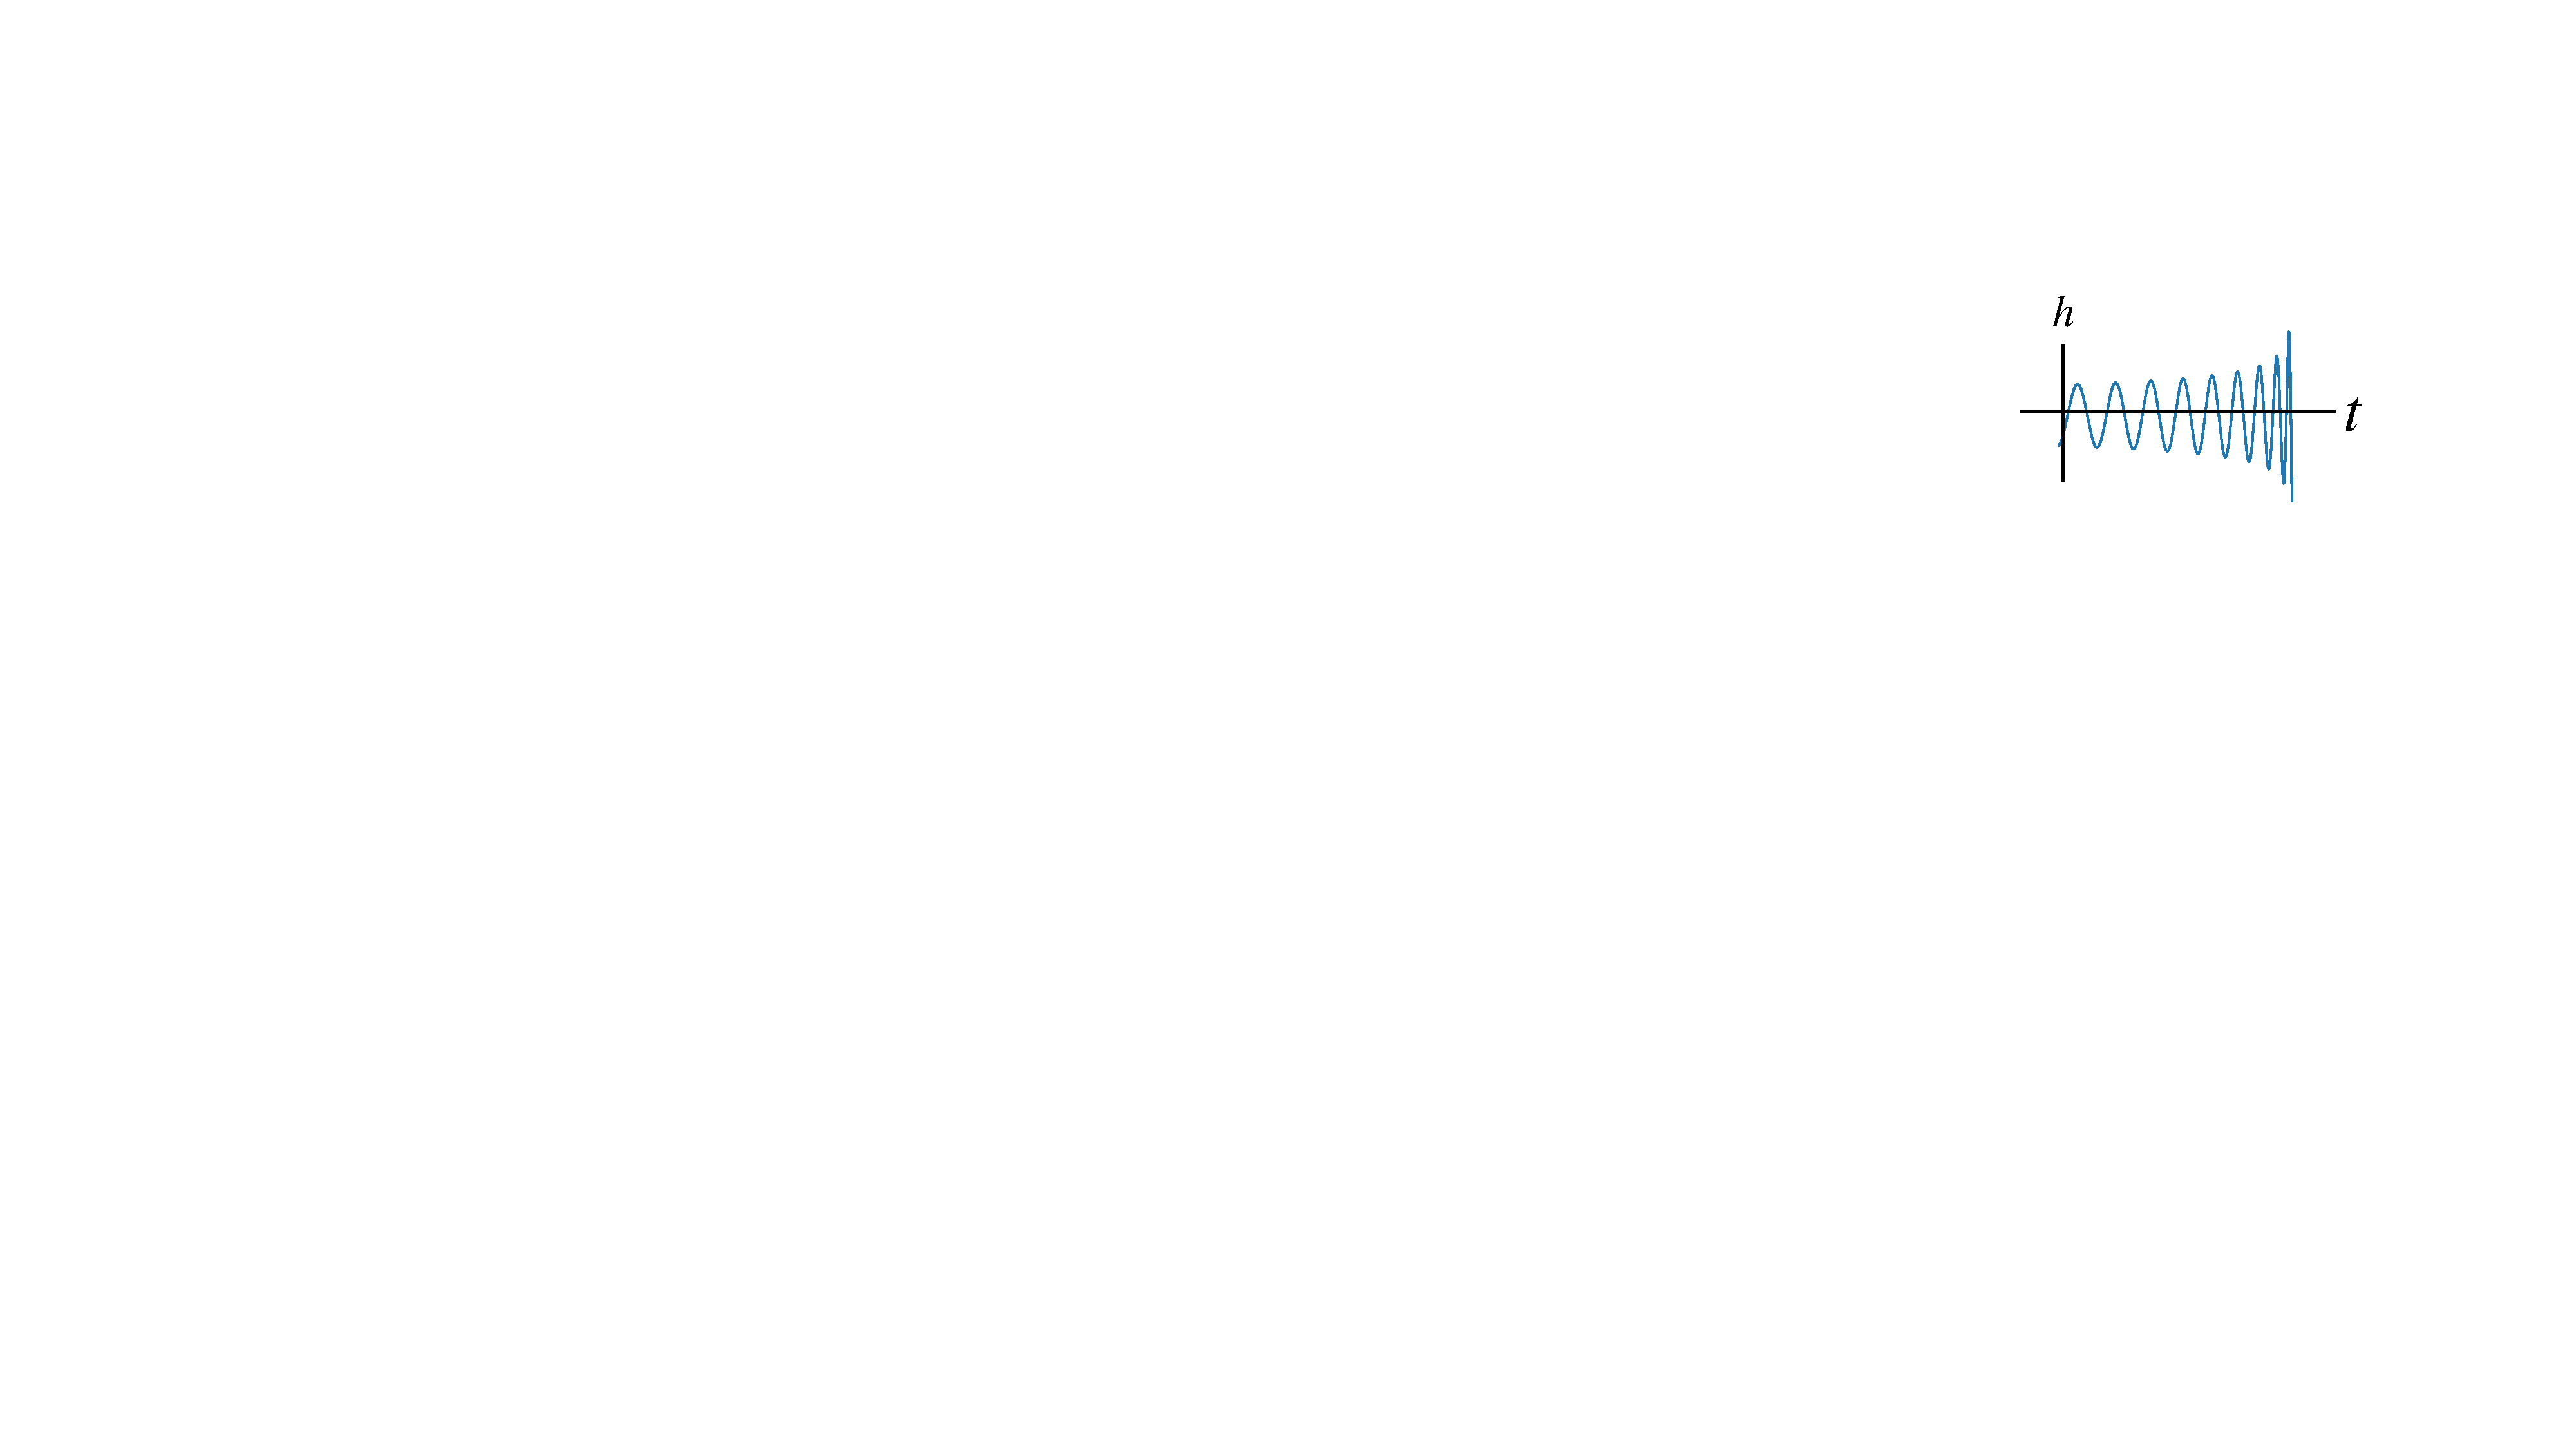
\includegraphics[width=0.25\textwidth]{Figures/chirp_prior}}
\hspace{1 in}
\subfigure[]{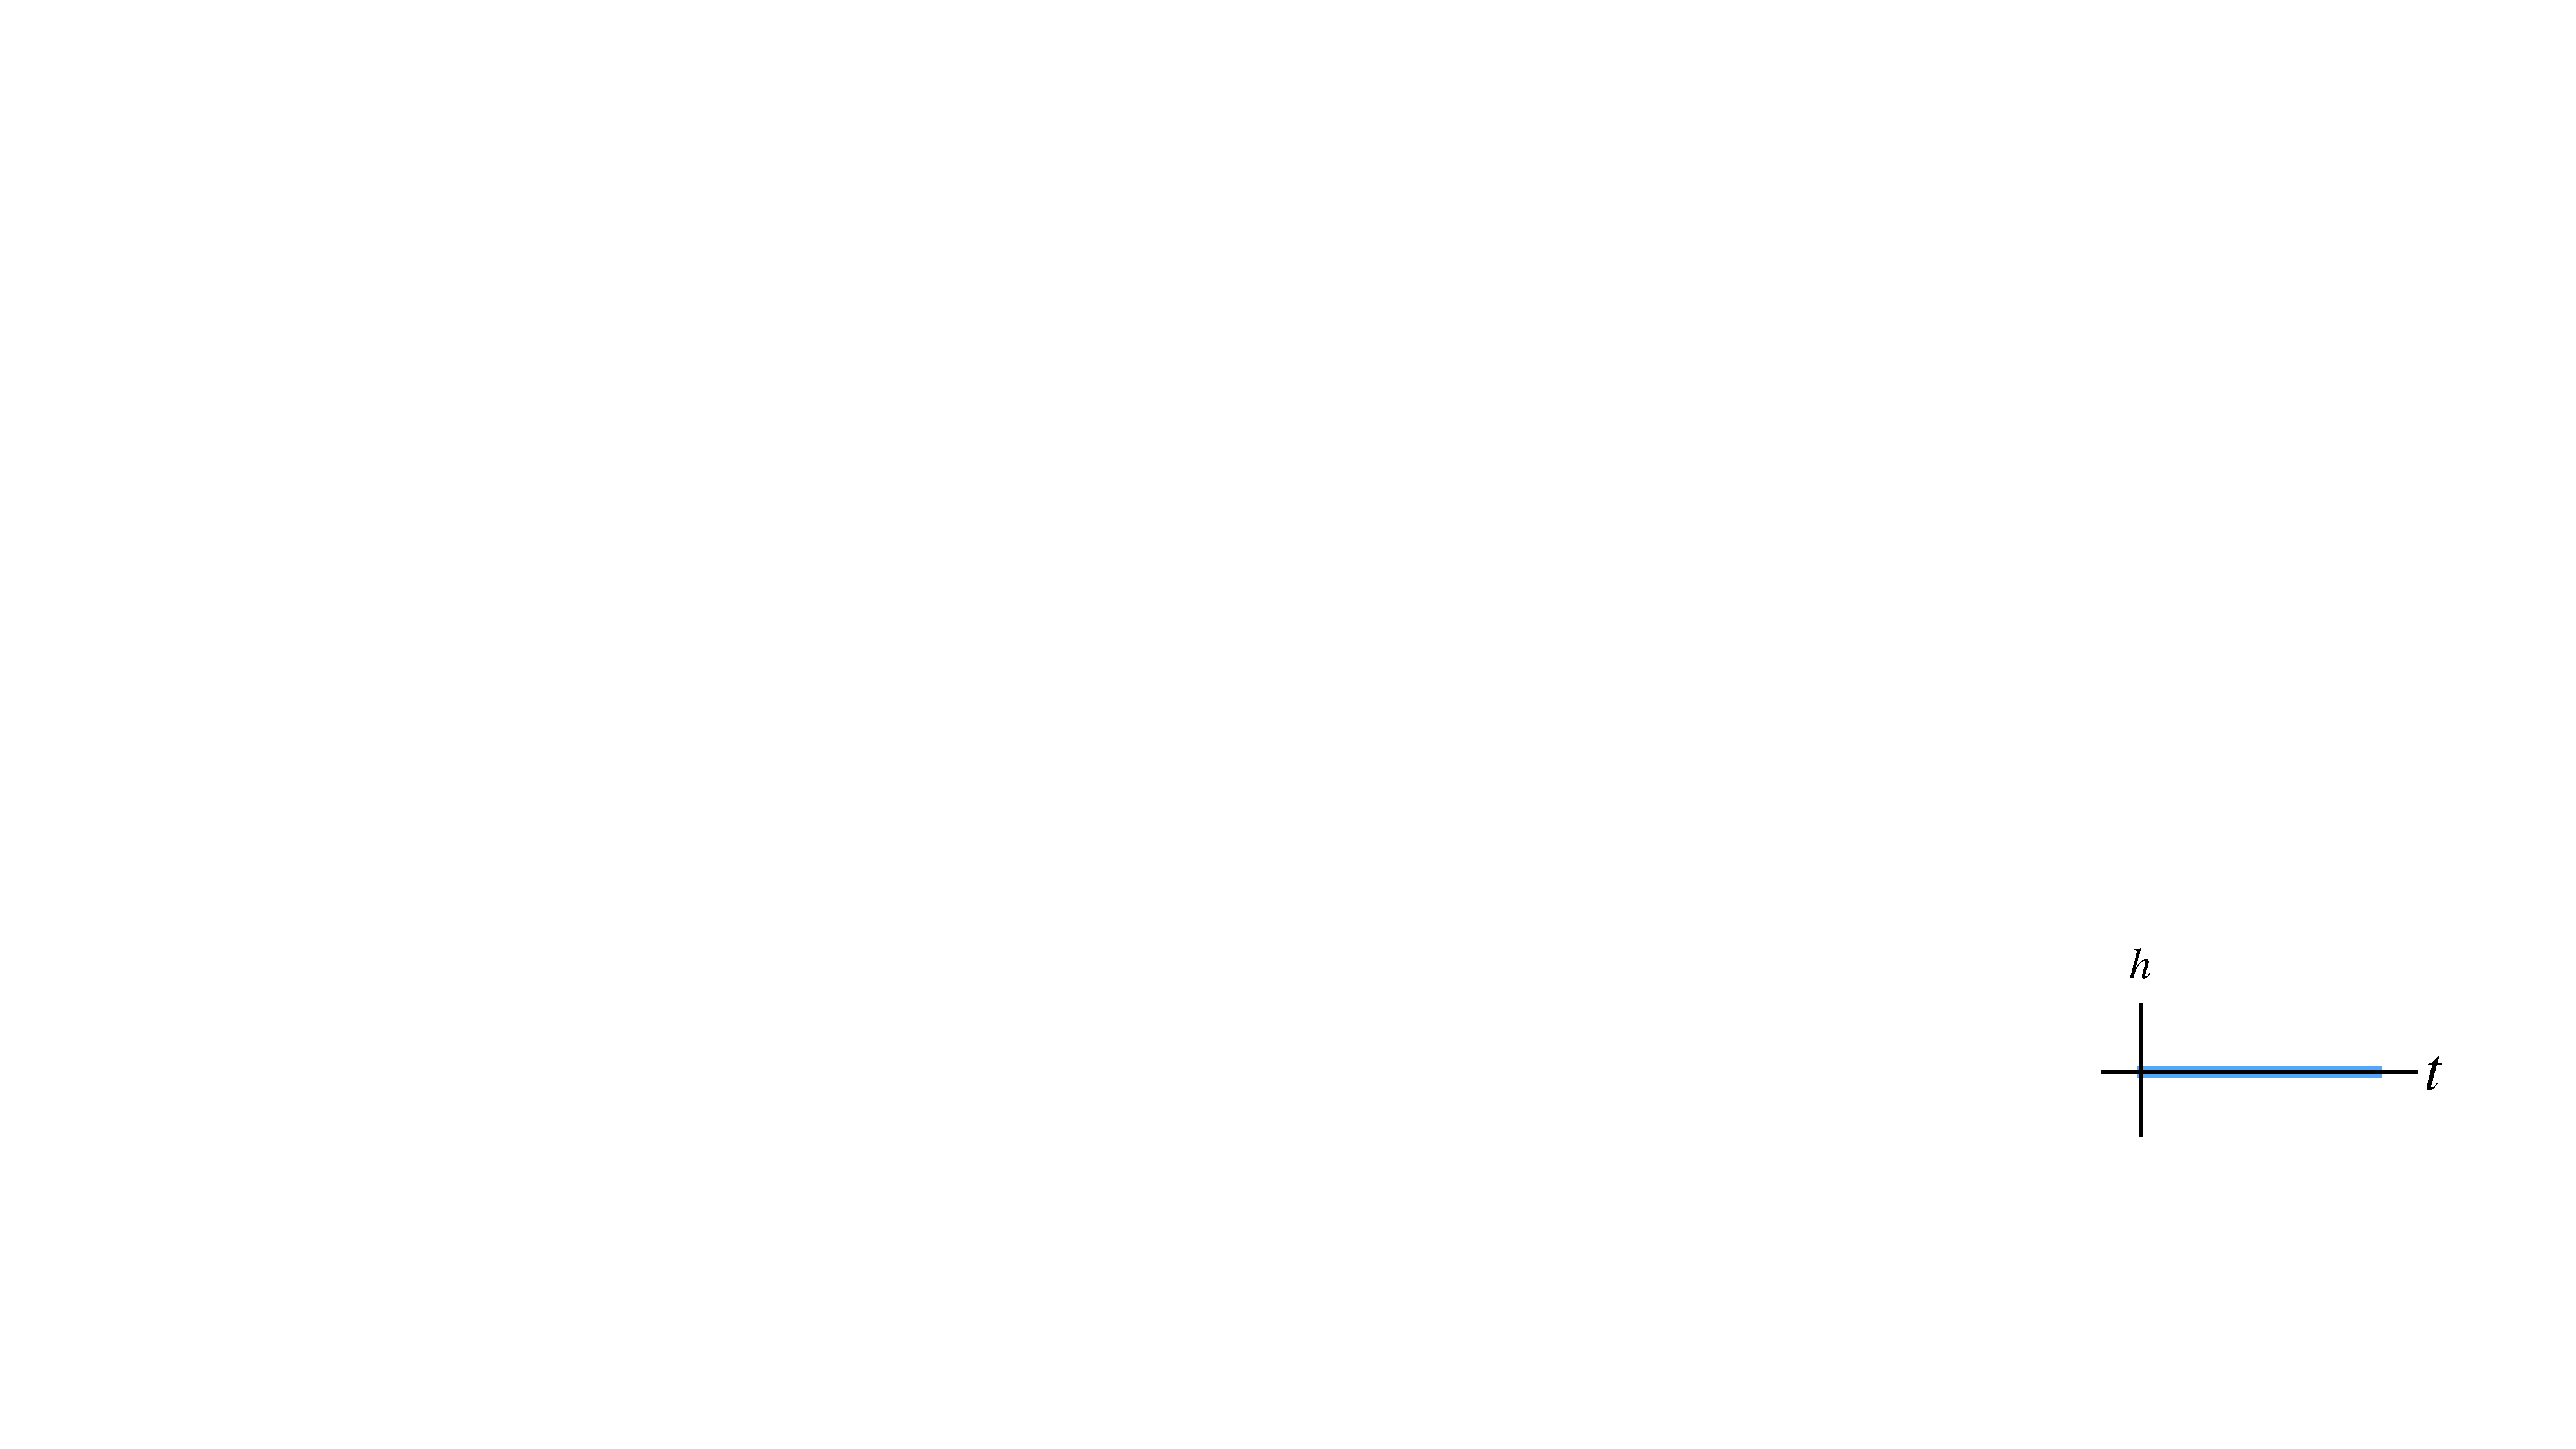
\includegraphics[width=0.25\textwidth]{Figures/no_signal_prior}}
\caption{The two components of the ``mixture" signal prior for the Bayesian 
BBH search.
Panel (a): With probability $\xi$, the signal prior for $h(t)$ is a 
chirp waveform.
Panel (b): With probability $(1-\xi)$, the signal prior for $h(t)$ is that
the signal is absent, i.e., $h(t)=0$.}
\label{f:mixture_signal_priors}
\end{center}
\end{figure}

\begin{figure}[htbp!]
\begin{center}
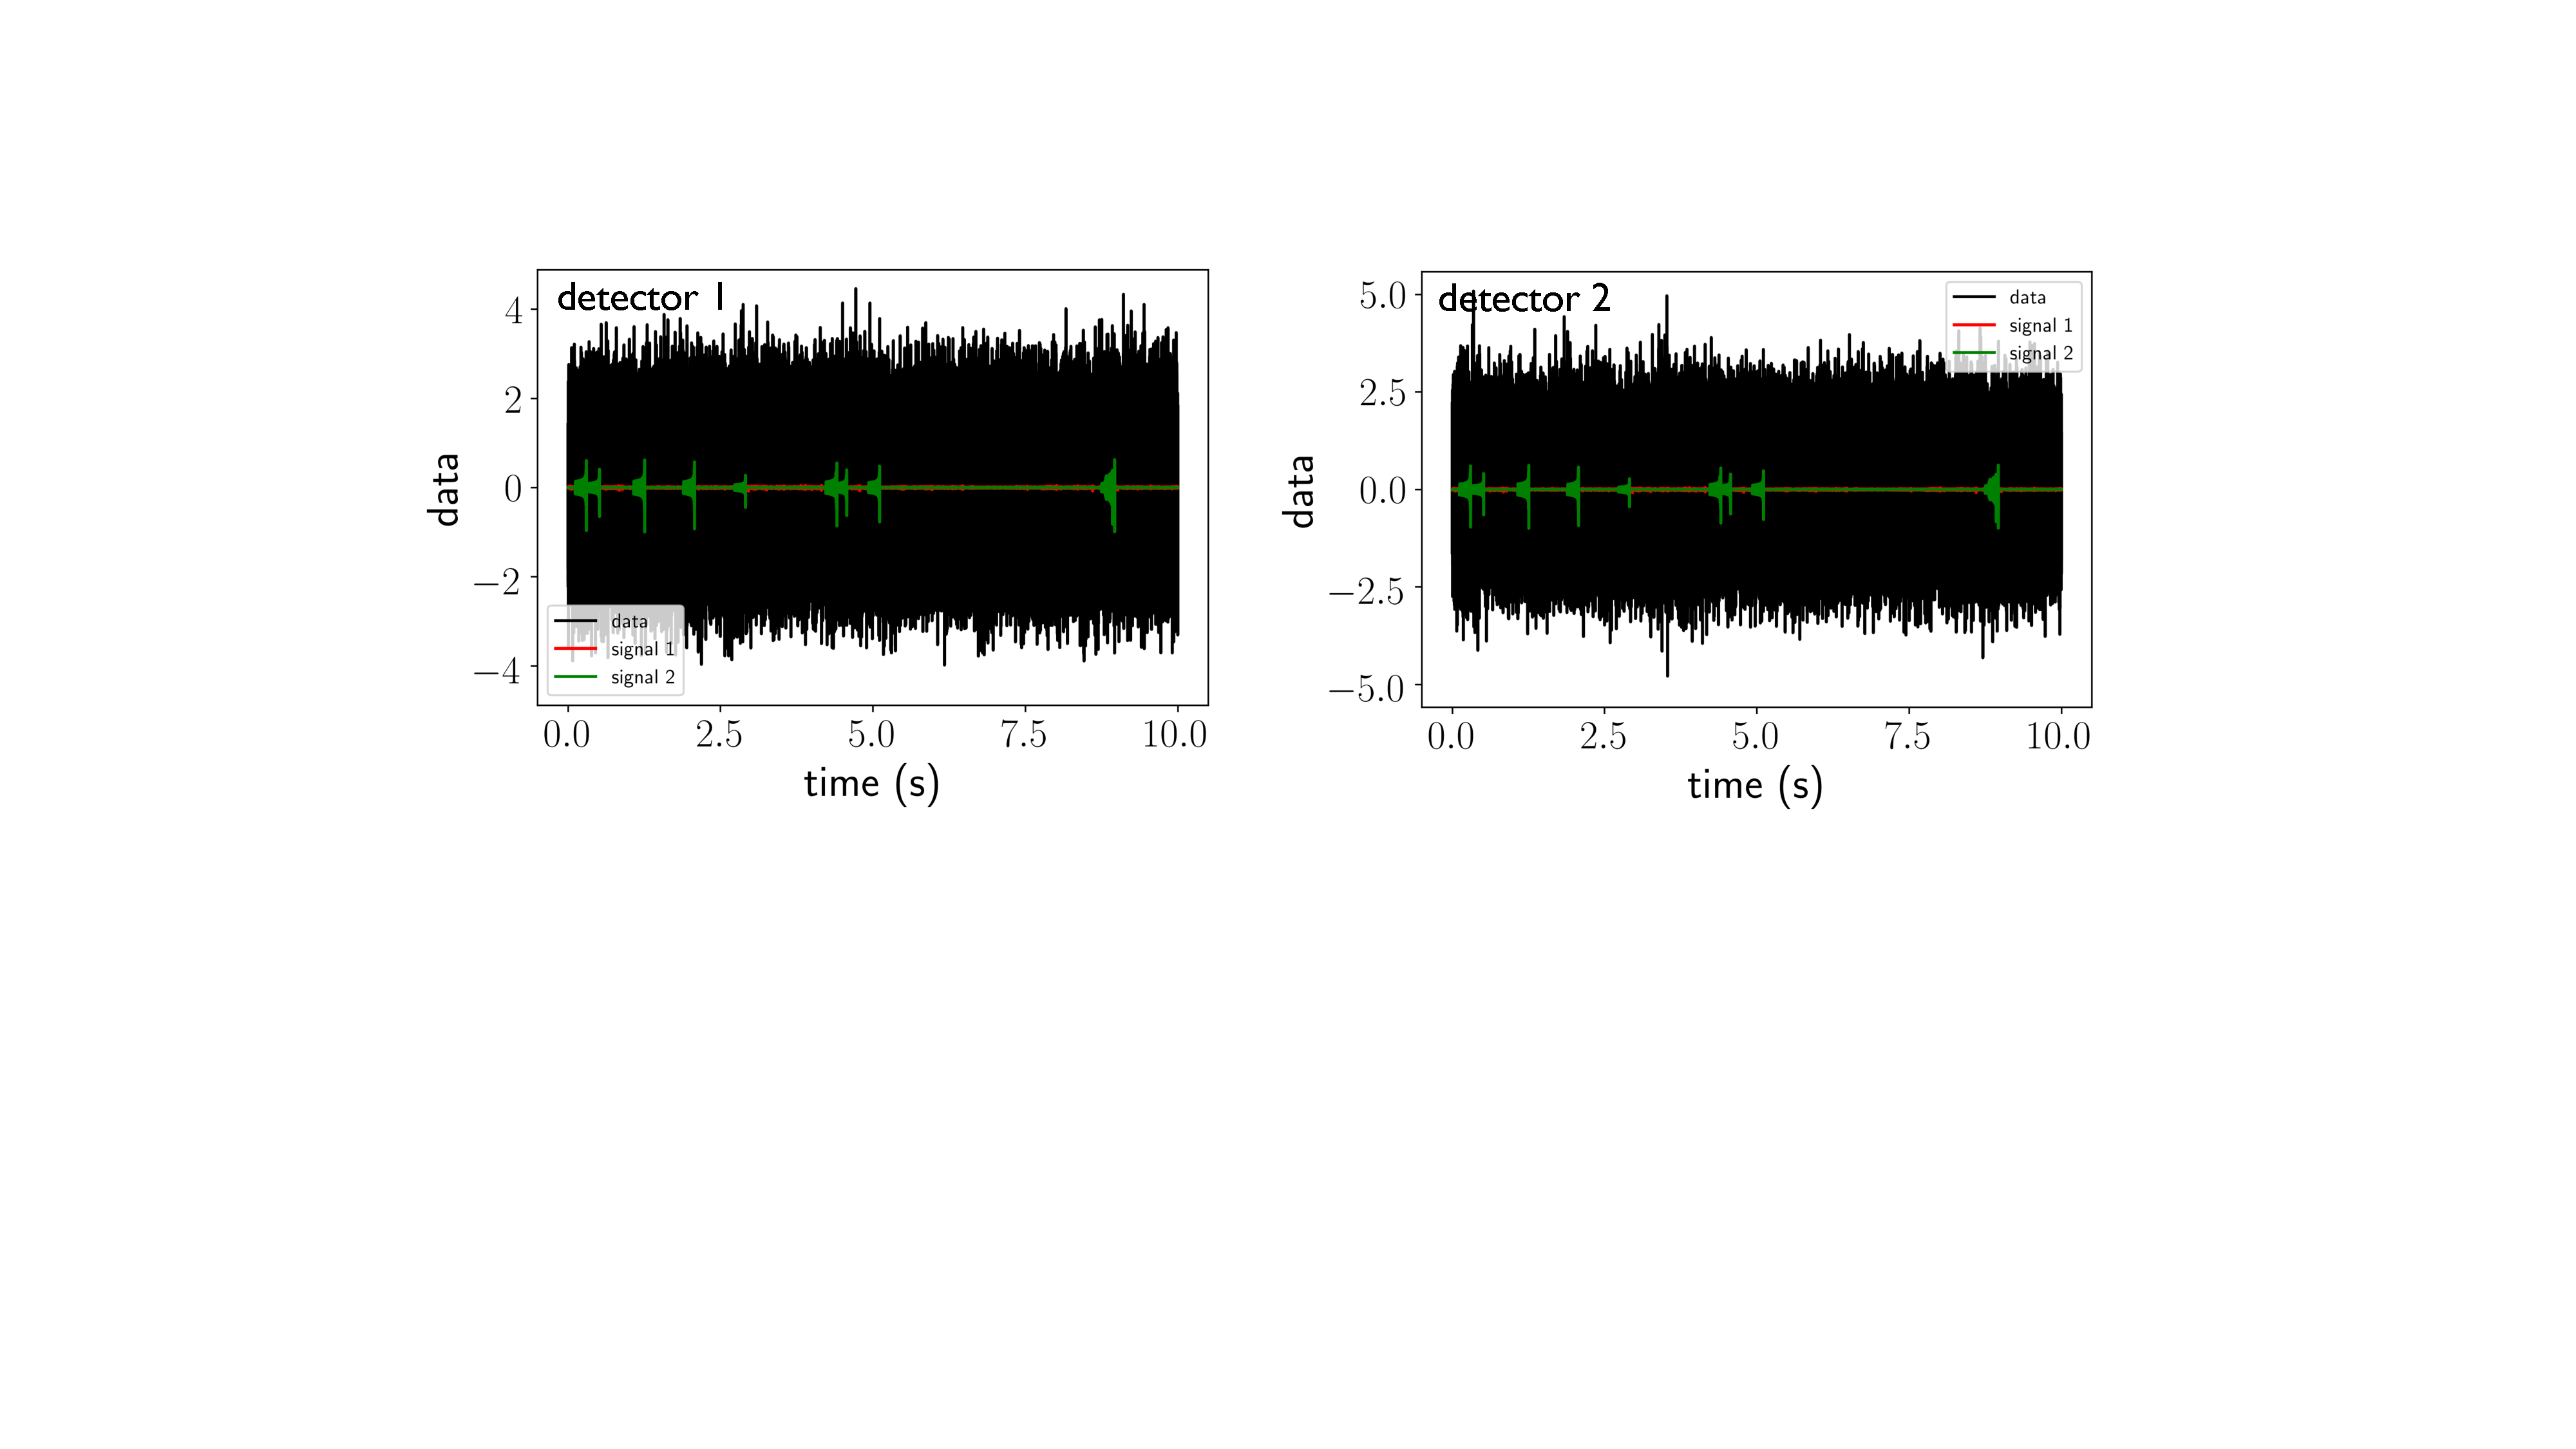
\includegraphics[width=\textwidth]{Figures/BBH-BNS-simulated-data}
\caption{Simulated BBH and BNS data in two coincident and coaligned
detectors.
The confusion-limited BNS background is shown in orange;
the popcorn-like BBH background is shown in green.
The black trace is the data consisting of the BBH and BNS signal
plus white Gaussian-stationary noise, uncorrelated in the two
detectors.}
\label{f:BBH-BNS-simulated-data}
\end{center}
\end{figure}

\begin{figure}[htbp!]
\begin{center}
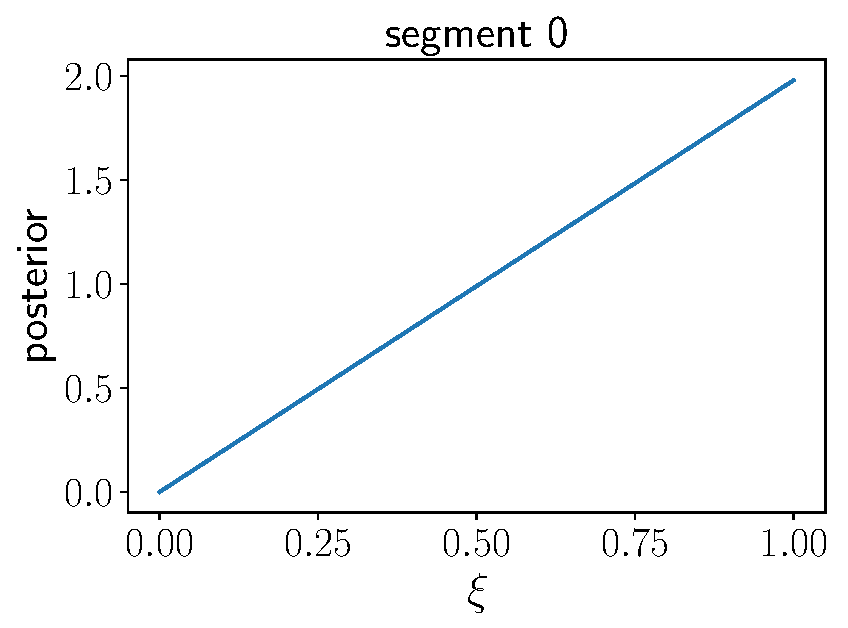
\includegraphics[width=0.24\textwidth]{Figures/posterior_xi_seg_0}
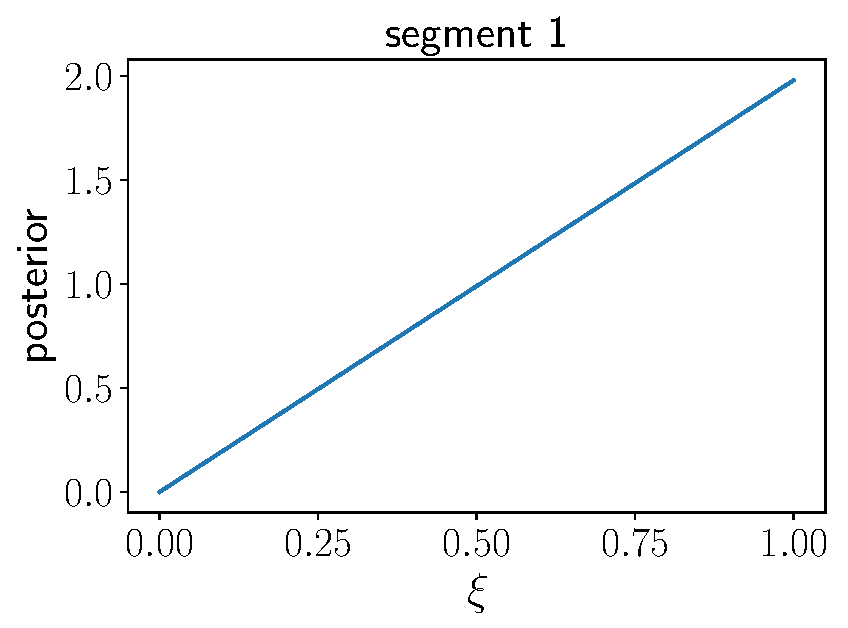
\includegraphics[width=0.24\textwidth]{Figures/posterior_xi_seg_1}
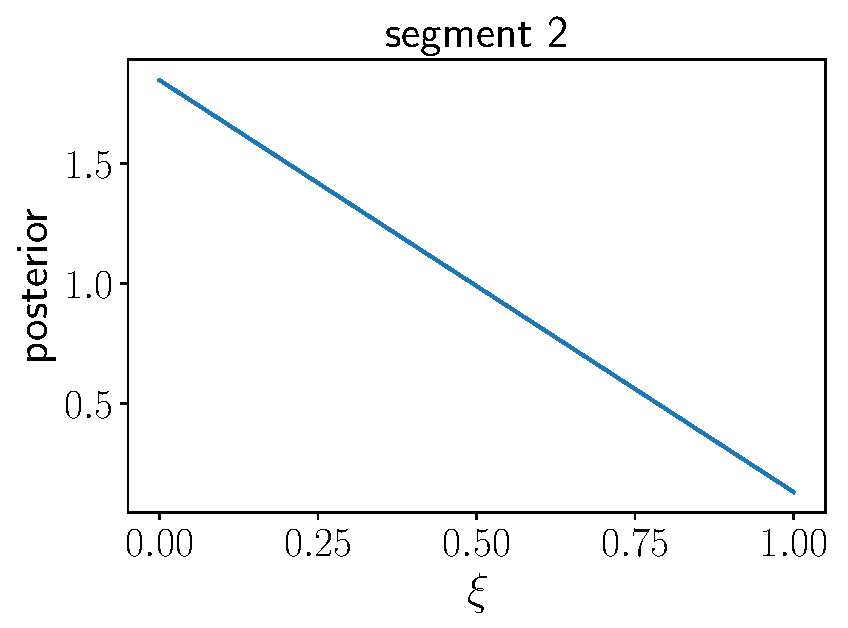
\includegraphics[width=0.24\textwidth]{Figures/posterior_xi_seg_2}
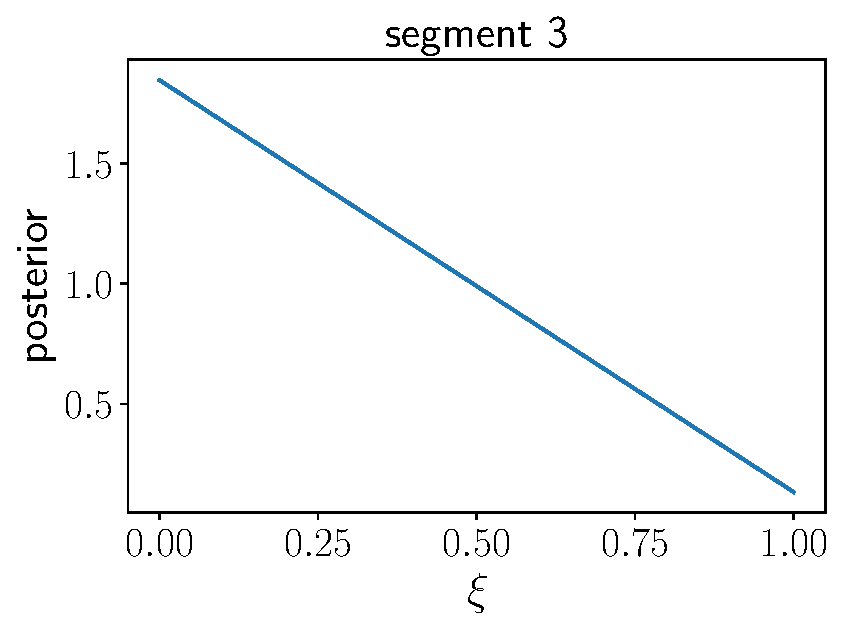
\includegraphics[width=0.24\textwidth]{Figures/posterior_xi_seg_3}
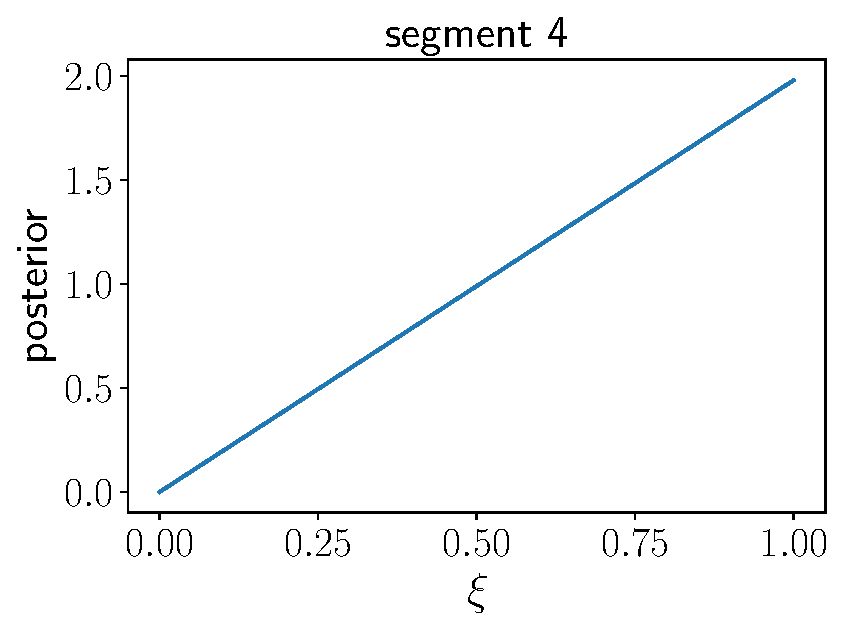
\includegraphics[width=0.24\textwidth]{Figures/posterior_xi_seg_4}
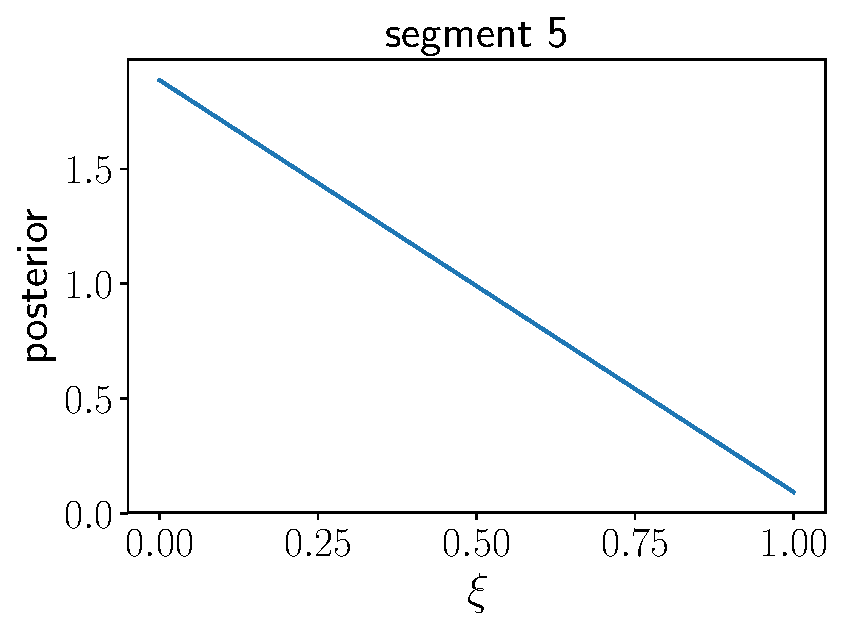
\includegraphics[width=0.24\textwidth]{Figures/posterior_xi_seg_5}
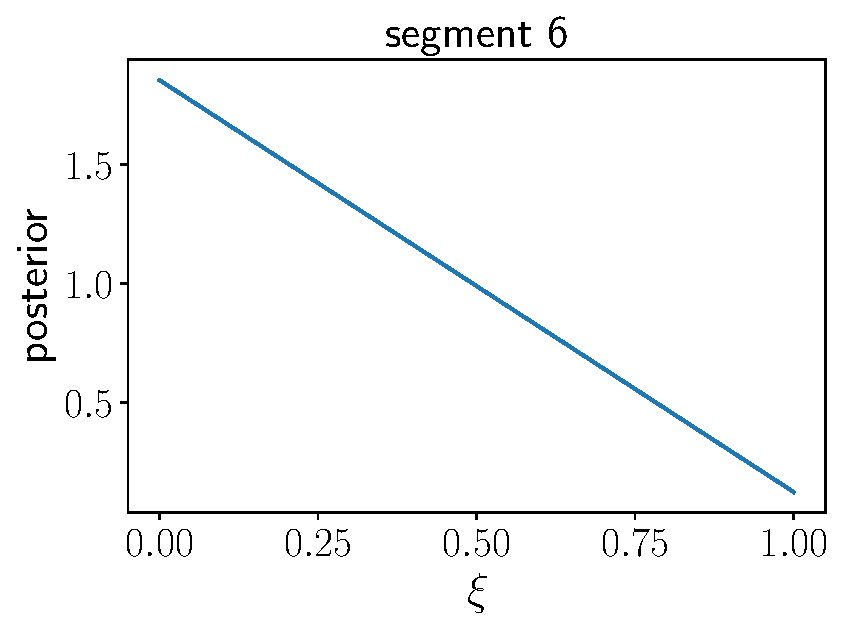
\includegraphics[width=0.24\textwidth]{Figures/posterior_xi_seg_6}
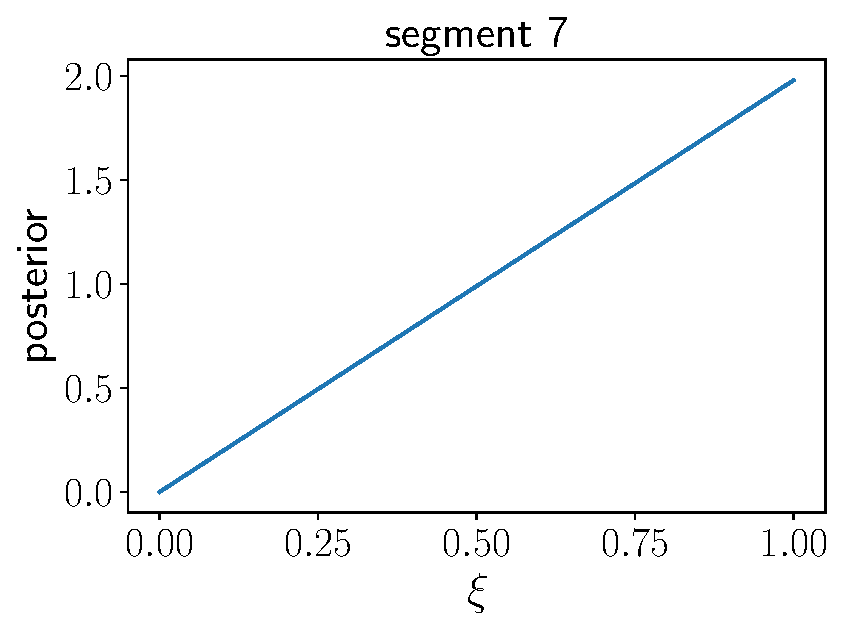
\includegraphics[width=0.24\textwidth]{Figures/posterior_xi_seg_7}
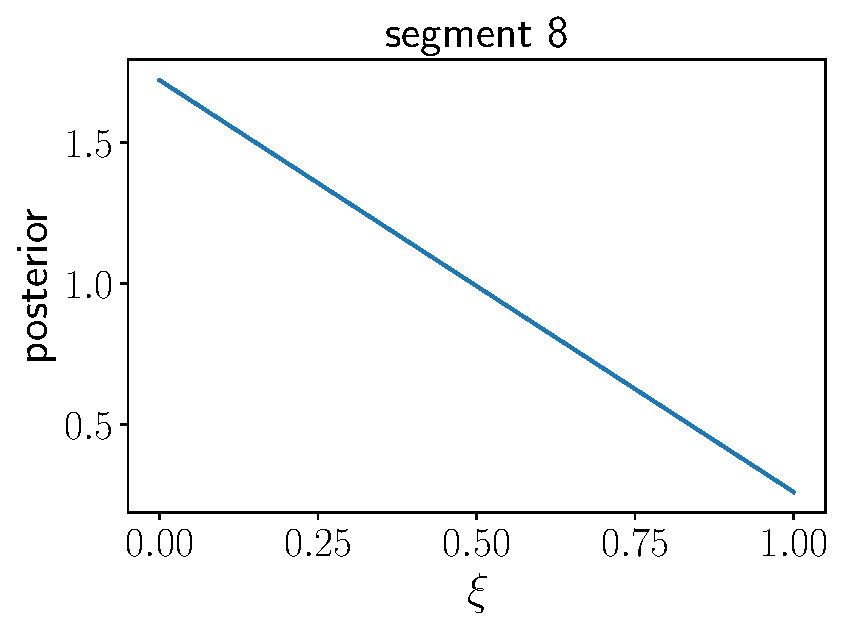
\includegraphics[width=0.24\textwidth]{Figures/posterior_xi_seg_8}
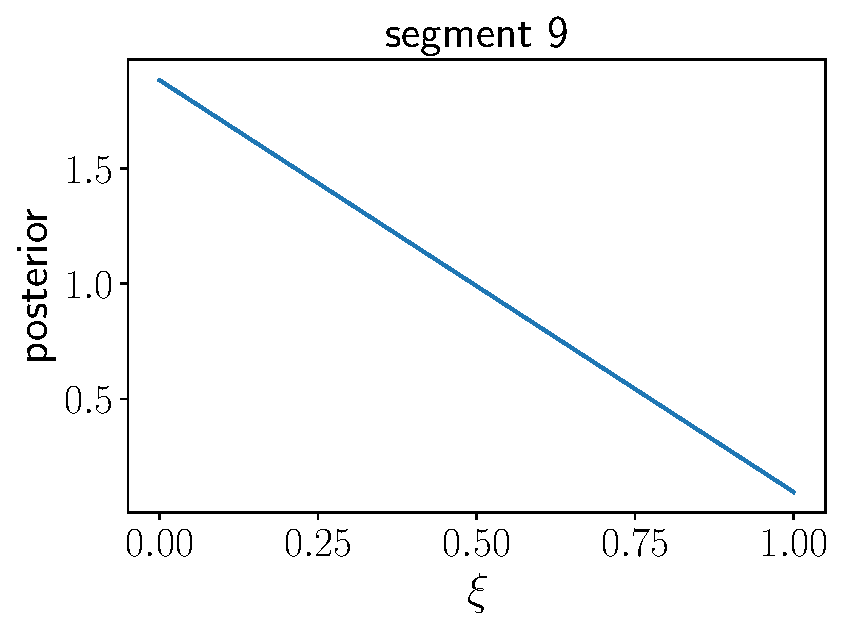
\includegraphics[width=0.24\textwidth]{Figures/posterior_xi_seg_9}
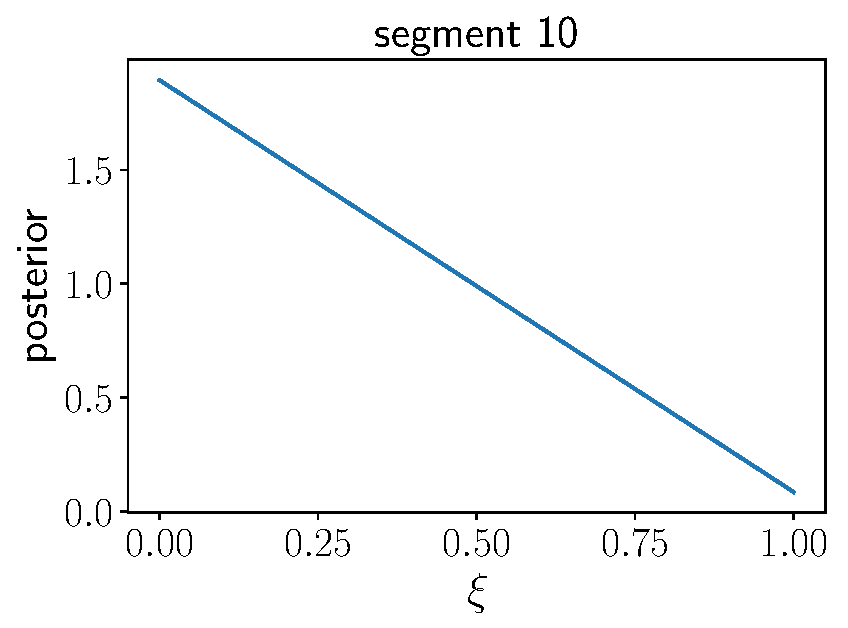
\includegraphics[width=0.24\textwidth]{Figures/posterior_xi_seg_10}
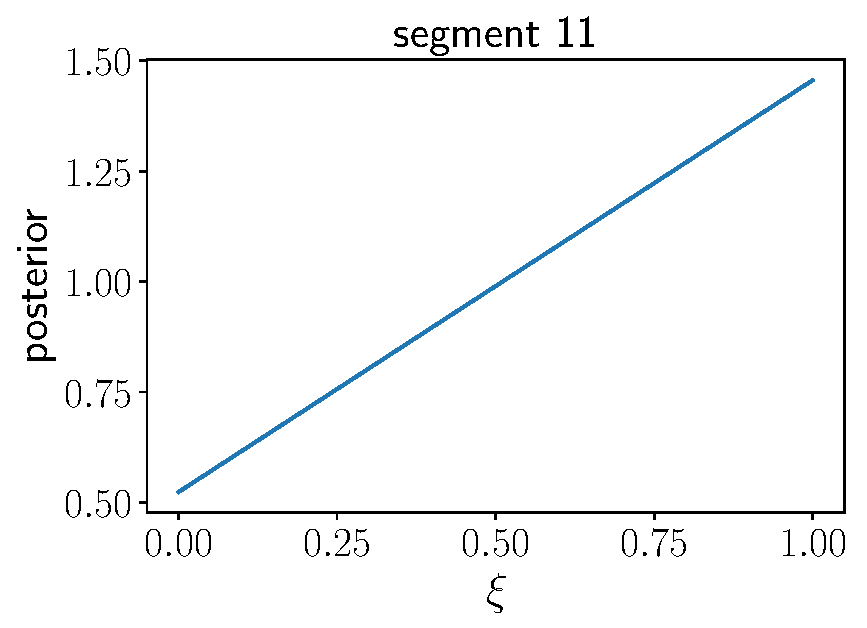
\includegraphics[width=0.24\textwidth]{Figures/posterior_xi_seg_11}
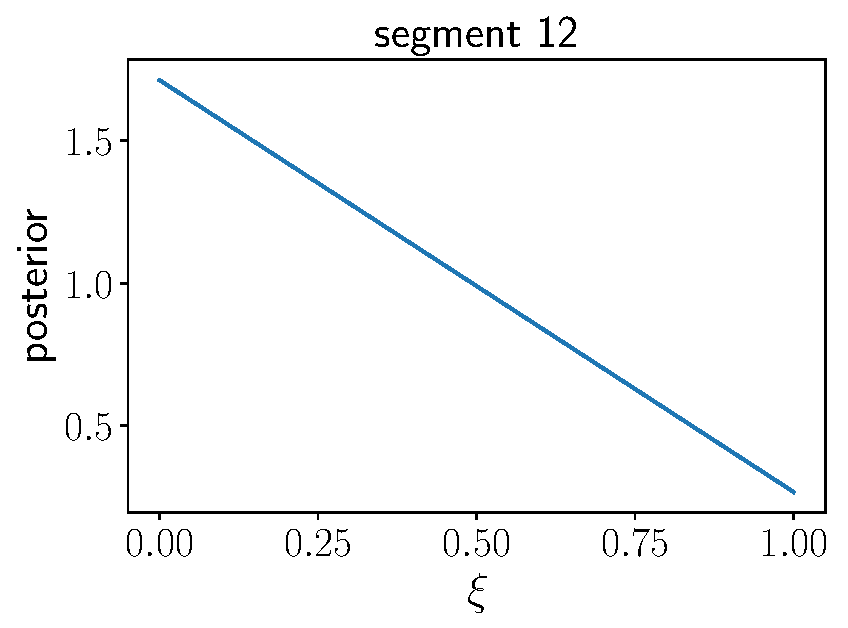
\includegraphics[width=0.24\textwidth]{Figures/posterior_xi_seg_12}
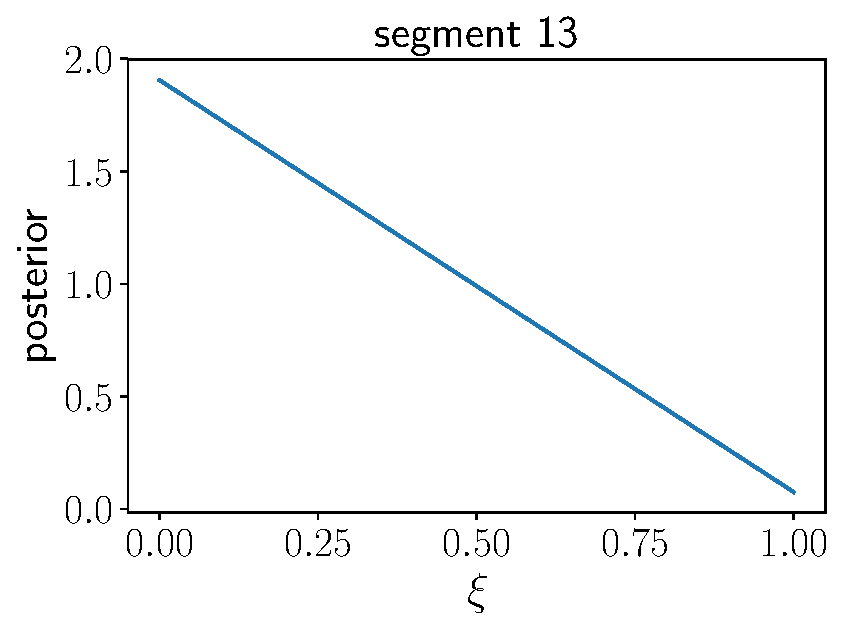
\includegraphics[width=0.24\textwidth]{Figures/posterior_xi_seg_13}
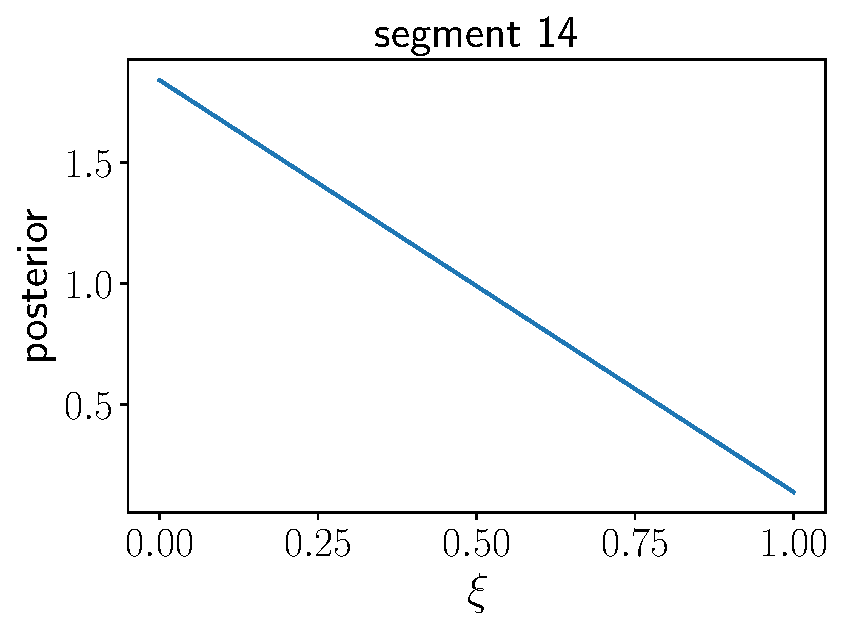
\includegraphics[width=0.24\textwidth]{Figures/posterior_xi_seg_14}
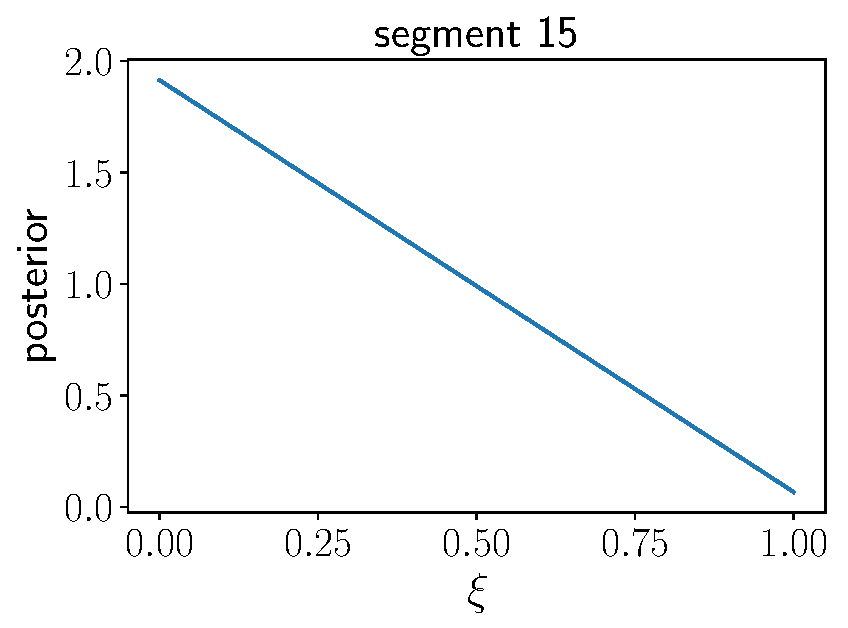
\includegraphics[width=0.24\textwidth]{Figures/posterior_xi_seg_15}
\caption{Posterior distributions for $\xi$ for the first 16 segments
(i.e., first 4~s) of data.}
\label{f:posteriors_xi_seg}
\end{center}
\end{figure}

\begin{figure}[htbp!]
\begin{center}
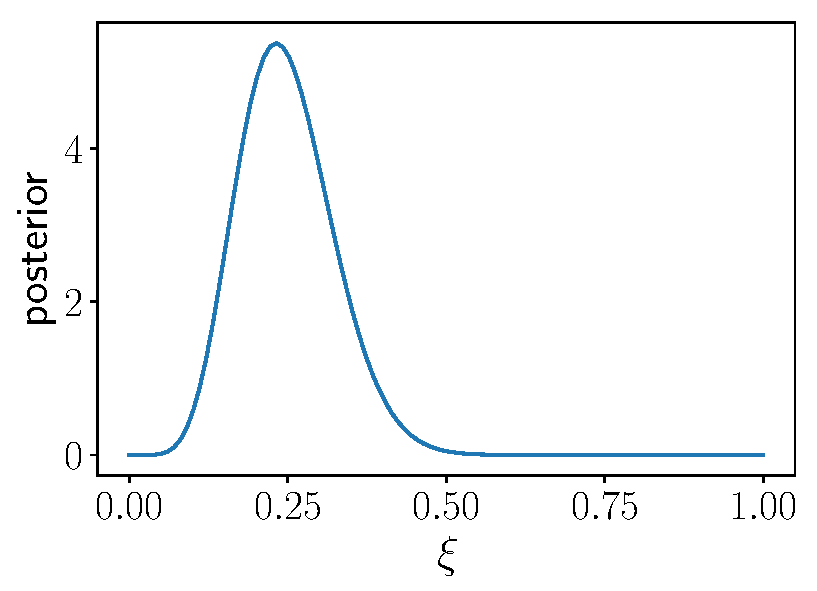
\includegraphics[width=0.5\textwidth]{Figures/posterior_xi}
\caption{The cumulative posterior distribution for $\xi$ after 
combining all 40~segments of data.}
\label{f:posterior_xi}
\end{center}
\end{figure}

\begin{figure}[htbp!]
\begin{center}
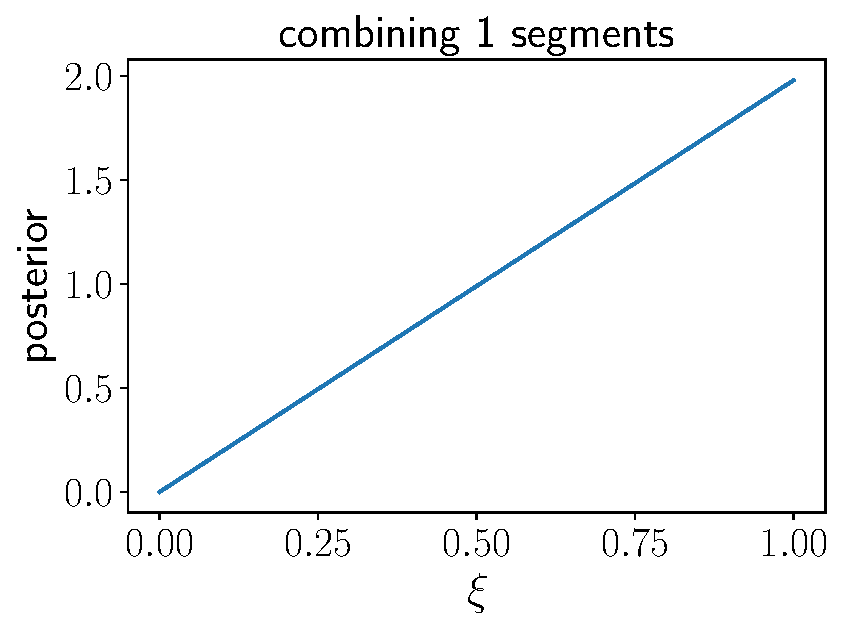
\includegraphics[width=0.24\textwidth]{Figures/posterior_xi_cum_0}
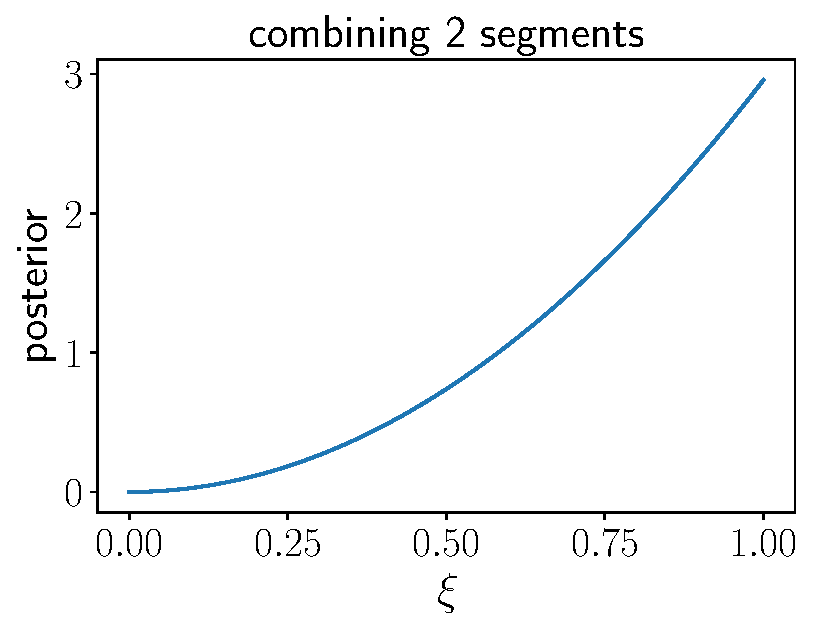
\includegraphics[width=0.24\textwidth]{Figures/posterior_xi_cum_1}
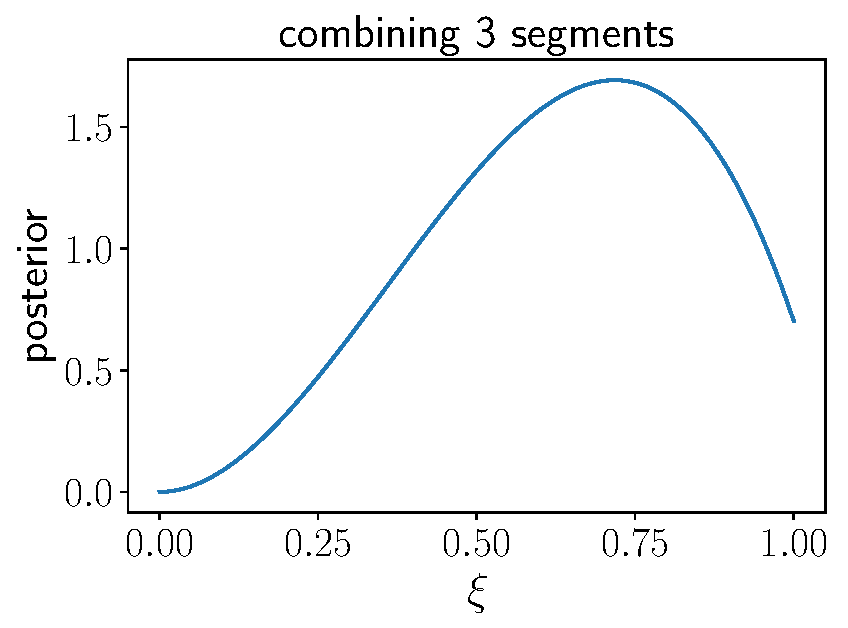
\includegraphics[width=0.24\textwidth]{Figures/posterior_xi_cum_2}
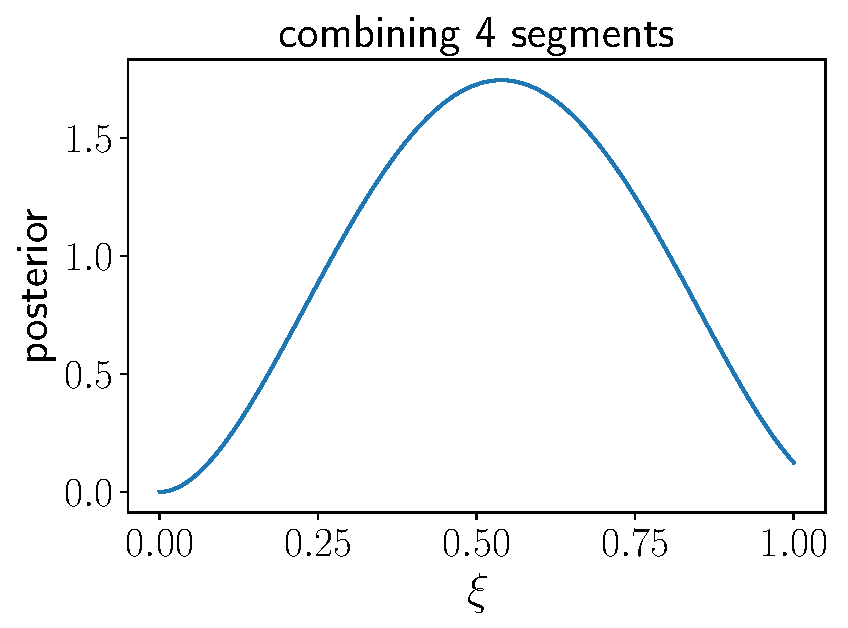
\includegraphics[width=0.24\textwidth]{Figures/posterior_xi_cum_3}
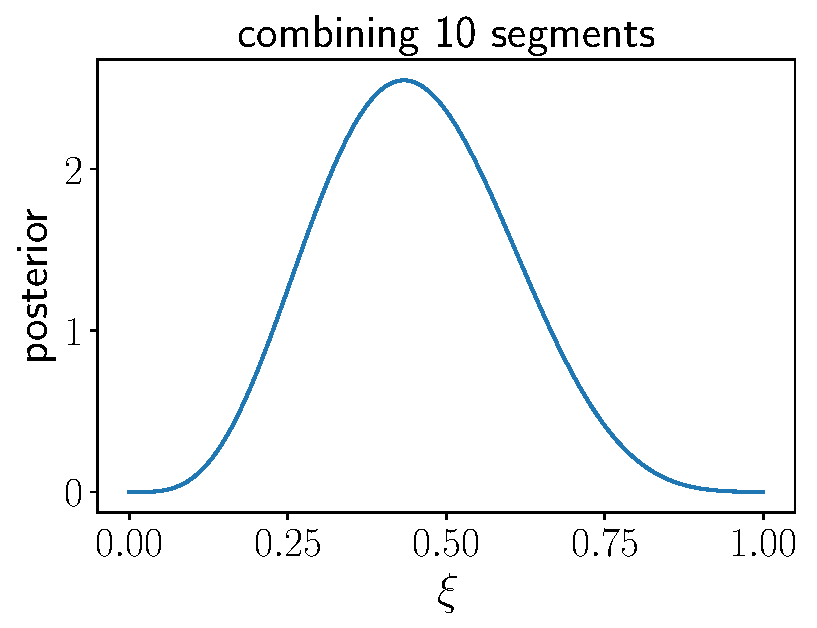
\includegraphics[width=0.24\textwidth]{Figures/posterior_xi_cum_9}
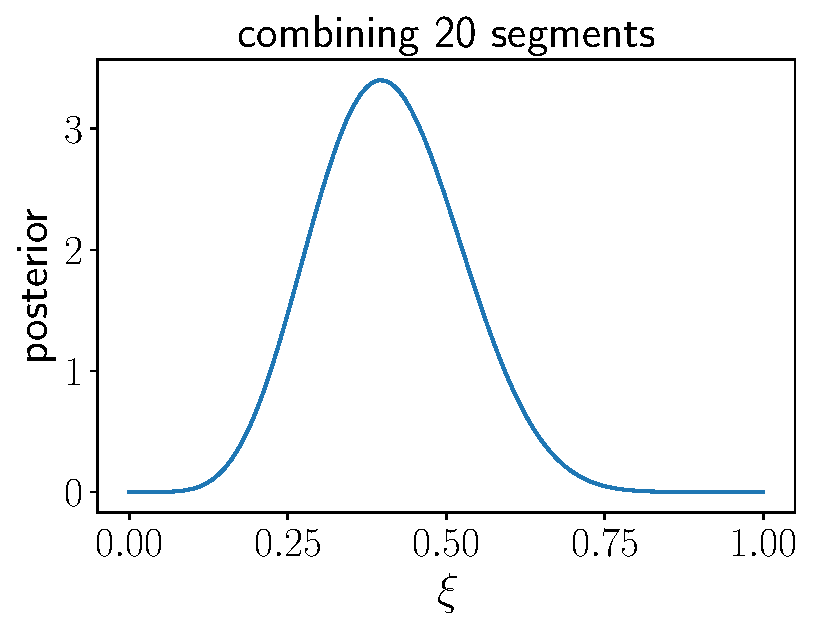
\includegraphics[width=0.24\textwidth]{Figures/posterior_xi_cum_19}
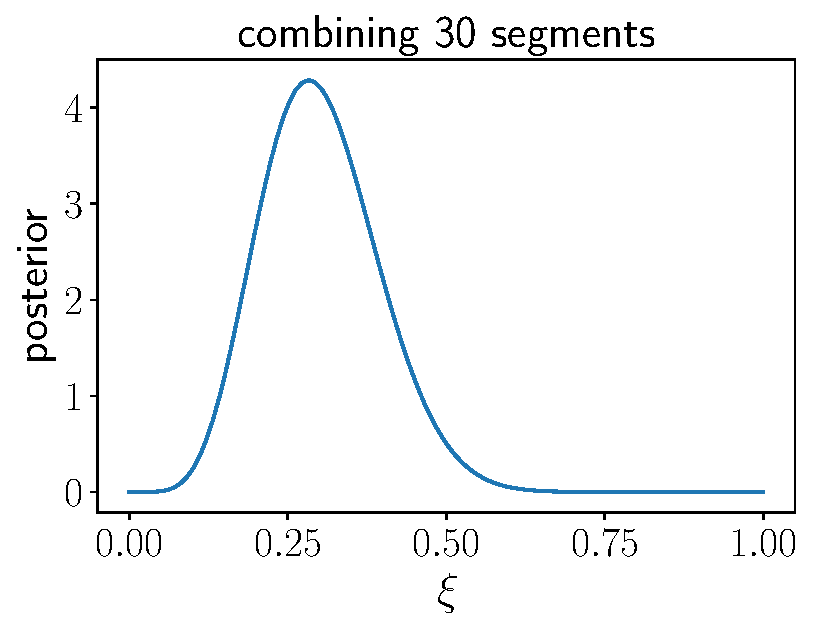
\includegraphics[width=0.24\textwidth]{Figures/posterior_xi_cum_29}
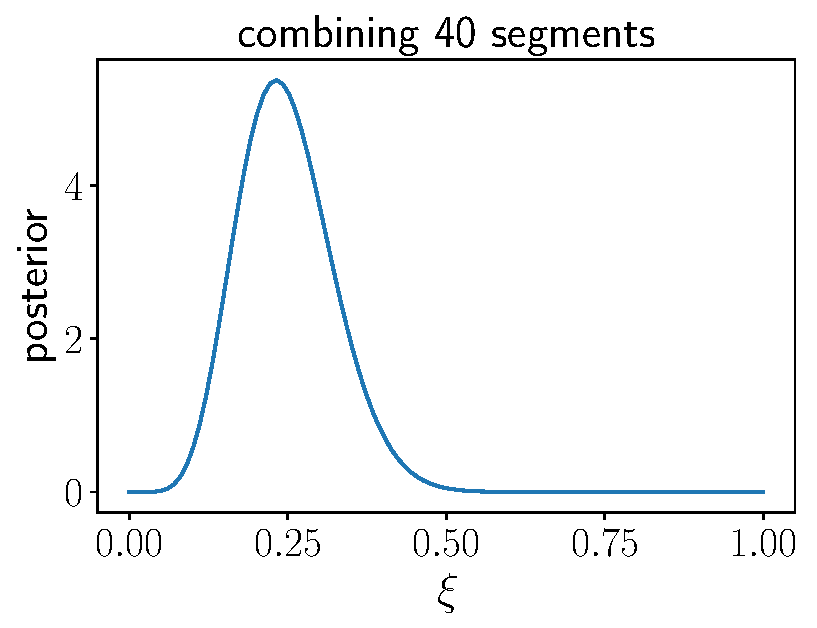
\includegraphics[width=0.24\textwidth]{Figures/posterior_xi_cum_39}
\caption{Cumulative posterior distributions for $\xi$ combining the
first $n$ segments of data.
The bottom-rightmost plot is also shown in Figure~\ref{f:posterior_xi}.}
\label{f:posteriors_xi_cum}
\end{center}
\end{figure}


